\documentclass[10pt, a4paper]{report}
\usepackage[paper=a4paper, left=1.5cm, right=1.5cm, bottom=1.5cm, top=3.5cm]{geometry}
\usepackage[utf8]{inputenc}
\usepackage[T1]{fontenc}
\usepackage[spanish]{babel}
\usepackage{indentfirst}
\usepackage{fancyhdr}
\usepackage{latexsym}
\usepackage{lastpage}
\usepackage{fancyhdr}
\usepackage[pdftex]{graphicx}
\usepackage{color}
\usepackage{dsfont}
\usepackage{xspace}
\usepackage{xargs}
\usepackage{listings} 
\usepackage{algpseudocode}
\usepackage{graphicx}
\usepackage{amsmath}
\usepackage{caption}
\usepackage{amssymb}
\usepackage{float}
\usepackage{sidecap}
\usepackage{textcomp}
\usepackage{fancybox}

\begin{document}

\newpage

\chapter*{Aclaraciones}

Este resumen fue hecho con el prop\'osito de volcar todo el conocimiento necesario para el final de algoritmos 2 a medida que estudiaba para el mismo. La motivaci\'on fue principalmente, y bajo mi criterio, porque notaba que la informaci\'on estaba segmentada y necesitaba un poco mas de organizaci\'on, especialmente los temas de especificaci\'on y dise\~no. Estos dos \'ultimos fueron principalmente extra\'idos de los apuntes de la c\'atedra, los cuales contienen la informaci\'on necesaria para entender perfectamente los temas mas ejemplos. De estos \'ultimos, quise organizarlos a mi modo, de forma resumida, removiendo los ejemplos y dejando solo los aspectos mas te\'oricos, y agregando algunas clarificaciones para algunos de los temas.

~

El resumen estar\'a dividido en ``cap\'itulos'', no porque sea un libro, sino por un tema de orden, ya que los temas quedan agrupados en cuatro categor\'ias generales. Las primeras dos, como dije anteriormente, sus referencias pueden ser encontradas en los apuntes correspondientes a cada tema, las diapositivas de las clases y algunos agregados de mi parte de apuntes o dudas que consulte y resolv\'i. En la tercera secci\'on, las definiciones de las clases de complejidad fue traducida directamente del Cormen[1], como as\'i tambi\'en las estructuras de datos como ABB, Heap arboles B y arboles Red-Black. Para las estructuras de datos de Splay Trees y arboles 234 (contenidos dentro de la secci\'on de arboles B), son pr\'acticamente una transcripci\'on de v\'ideos de clases de la universidad de Berkeley[2] correspondientes a los temas. Finalmente, en la cuarta secci\'on los temas de Dividir y Conquistar y c\'odigos de Huffman, fueron traducidos del Cormen directamente, junto a las definiciones del Teorema Maestro y \'arbol de recurrencia, los temas de ordenamiento son nuevamente transcripciones de clases de Berkeley[3].

~

Si bien este resumen intento hacerse a conciencia y con la m\'axima correctitud y verificaci\'on posible, es muy probable que el mismo contenga errores. Es por ello que pido encarecidamente que de encontrarlos sean corregidos o al menos dar una advertencia de los mismos. El c\'odigo fuente de este archivo, el cual fue producido en LaTeX, estar\'a disponible en mi cuenta de GitHub[4], junto con las instrucciones para modificarlo. Ah\'i mismo tambi\'en se podr\'a dar notificaci\'on de los errores encontrados, como tambi\'en a mi cuenta de mail[5] si les es mas c\'omodo.

\tableofcontents

\chapter{Tipos Abstractos de Datos}

\section{Introducci\'on y noci\'on}
Los tipos abstractos de datos (TADs) son modelos matem\'aticos que se construyen con el fin de exponer los aspectos relevantes de un problema bajo an\'alisis. La raz\'on por la cual son usados es porque gracias a los mismos es posible realizar un an\'alisis exhaustivo junto con la comprensi\'on cabal del funcionamiento del objeto de estudio, esto se logra utilizando la abstracci\'on como herramienta para lograr la comprensi\'on y mediante conceptos claves como lo son el encapsulamiento, podremos resaltar las cualidades relevantes de lo que queremos analizar.

De cierta forma lo que queremos lograr es capturar lo m\'as fielmente posible, y con precisi\'on matem\'atica, un problema, para el que luego encontraremos una soluci\'on. Es importante tener en cuenta que en la etapa de especificaci\'on solo debe preocuparnos describir el problema que se intenta resolver, y no sus eventuales soluciones.

\section{Sintaxis y sem\'antica de un TAD}

Todo lenguaje tiene una gram\'atica o sintaxis, las cuales son un conjunto de reglas que indican c\'omo se escriben las oraciones del lenguaje y las reglas sem\'anticas, que indican c\'omo deben interpretarse las oraciones v\'alidas del lenguaje. Los lenguajes l\'ogicos no son una excepci\'on a estas.

\subsubsection*{Sintaxis}

Para determinar un TAD, utilizaremos especificaciones de TADs (de la misma forma que se usan axiomas para caracterizar estructuras matem\'aticas). Para especificar un TAD es necesario definir:

\begin{itemize}
 \item La \textbf{signatura} que exponen las operaciones y que aridad tienen los modelos.
 \item Los \textbf{axiomas} son formulas bien formadas seg\'un ciertas reglas (sint\'acticas) que determinan el comportamiento de las operaciones.
\end{itemize}

\subsubsection*{Sem\'antica}

La sem\'antica declara con precisi\'on qu\'e cosas son modelos de nuestra teor\'ia, es decir le da un significado a las cosas que se pueden escribir de acuerdo a las reglas sint\'acticas. Un modelo de de nuestra teor\'ia es un ente matem\'atico tal que cumple que cada uno de sus conjuntos corresponden con un g\'enero del TAD y cada funci\'on con una operaci\'on, nosotros definiremos nuestro TAD de forma tal que acomodar\'a los modelos matem\'aticos que se ajusten a el, de cierta forma la especificaci\'on del TAD funciona como un descriptor del modelo matem\'atico. Un modelo matem\'atico determina qu\'e elementos del mundo real estar\'an reflejados en la especificaci\'on y que operaciones se permitir\'a realizar sobre ellos. 

Por otro lado una teor\'ia es consistente cuando en ella no existe una igualdad que afirme que \textbf{verdadero} es \textbf{falso}. Si introducimos una teor\'ia inconsistente al TAD provocara que no haya un modelo que se ajuste al mismo, y por lo tanto, y burdamente dicho, provocar\'a que el TAD no tenga sentido alguno ya que ning\'un modelo se ajustara a el y en consecuencia no seremos capaces de modelar nada.

Las instancias de un TAD son las que representan, mediante la abstracci\'on, un objeto de la vida real y cualquier modelo que sea descripto por un TAD especifico representa a todas las instancias posibles del objeto modelado. Es interesante remarcar que cuando nos referimos a instancias podemos estar hablando del mismo objeto y su evoluci\'on con respecto al tiempo, esto tambi\'en es modelable y podremos definir una instancia del objeto para cada instante de tiempo (o al menos para los cambios relevantes que queramos observar mediante el modelo).

\section{Conceptos a tener en cuenta}
\subsection{Metalenguaje}

Muchas veces al intentar describir propiedades acerca de un lenguaje formal no nos alcanza con dicho lenguaje, y es por ello que necesitamos de un metalenguaje para lograrlo. En las especificaciones de TADs, el metalenguaje es utilizado para escribir las restricciones de las funciones y para describir la igualdad observacional.

\subsection{Restricciones sobre funciones totales}

En el formalismo de los tipos abstractos de datos s\'olo se permite especificar funciones totales, es decir aquellas que est\'an definidas para todo su dominio. Lo que t\'ecnicamente estamos haciendo no es restringir el dominio de las funciones sino definirlas s\'olo para la parte del dominio que nos interesa (por este motivo utilizaremos predicados del metalenguaje para restringirlas), o dicho de otra forma no diremos que valores toma la funci\'on cuando sus par\'ametros no cumplen con la restricci\'on. 

En consecuencia, cuando utilizamos una restricci\'on estaremos subespecificando. Las restricciones son una parte fundamental del TAD, con ellas explicitamos los casos para los cuales ciertas operaciones no tienen sentido (por el marco del problema o por una limitaci\'on t\'ecnica) y aportan claridad y coherencia a una especificaci\'on, por ello en este caso estaremos haciendo un uso l\'icito de la subespecificaci\'on. De cierta forma las restricciones nos permiten limitar el universo al cual aplican ciertas operaciones de nuestros TADs.

~

Es importante remarcar el caso cuando utilizamos una funci\'on con su dominio restringido $g(x)$ dentro de la definici\'on de otra funci\'on $h(x)$. Cuando sucede esto tendremos que asegurarnos de no llamar a $g$ con par\'ametros de su dominio que est\'en restringidos. Para evitar esto y lograr que $h$ este bien definida tendremos dos opciones. La primera consiste en agregar las restricciones necesarias a $h$ para no llamar a $g$ con par\'ametros restringidos, y la segunda, que es pr\'acticamente lo mismo pero desde otra perspectiva, es manejar la parte conflictiva del dominio de $h$, es decir aquellos valores de los par\'ametros de $h$ en donde llamar\'iamos a $g$ de forma ilegal, mediante un condicional en $h$ para efectuar otras operaciones o hacer un ajuste antes de llamar a $g$ de forma tal de no producir ninguna violaci\'on. Dicho de otra forma esto ultimo seria como definir a $h$ como una funci\'on partida.

\subsection{Incertidumbre mediante subespecificaci\'on}

Las restricciones nos servir\'an para expresar sobre que valores de los par\'ametros de una funci\'on determinada no daremos ninguna descripci\'on, sin embargo es por ello que tambi\'en deberemos asegurarnos de que si determinado valor de los par\'ametros de una operaci\'on es v\'alido de acuerdo a las restricciones, este indicando mediante los axiomas, cu\'al es el resultado para aquellos valores. En algunos casos no diremos exactamente qu\'e resultado da la funci\'on, si no que indicaremos qu\'e caracter\'isticas tiene ese resultado.

~

Esto \'ultimo es un concepto sutil y avanzando que a veces tambi\'en recibe el nombre de subespecificaci\'on y solo comparte el nombre con el descripto en al secci\'on anterior. La intenci\'on que reside detr\'as de el es la de dejar algunos aspectos particulares del TAD sin una definici\'on precisa, lo cual se convierte en un recurso muy \'util para manejar algunas incertidumbres de forma pr\'actica. La forma de lograr esto es caracterizando el resultado de una funci\'on de forma d\'ebil. Un ejemplo especifico de los tipos b\'asicos es la operaci\'on \textbf{dameUno} del tipo \textbf{conjunto}, la cual lo \'unico que nos dice es que nos devolvera un elemento perteneciente al conjunto sin especificar bajo que criterio lo har\'a. Esto significa que cualquier forma de elecci\'on que se decida implementar al conjunto va a ser apropiada, mientras que satisfagan la caracter\'istica de elegir un elemento del conjunto.

\subsection{No existe el orden de evaluaci\'on}
En algunos lenguajes de programaci\'on una funci\'on puede estar definida en partes y las partes de la misma pueden estar ordenadas mediante un orden de evaluaci\'on. Esto de alguna forma simplifica el esquema de evaluaci\'on de las funciones, ya que en vez de usar condicionales en la funci\'on y sobre los datos, podremos usar m\'ultiples definiciones a las que un dato se ajustara dependiendo si el pattern matching lo detecta como v\'alido y en donde la evaluaci\'on terminar\'a con la primer coincidencia, es decir con la primer definici\'on en el orden de evaluaci\'on que sea v\'alida para el dato. En estos casos las funciones se suelen ordenar desde los casos mas particulares hacia los casos mas generales.

En la especificaci\'on de los TADs la idea del pattern matching todav\'ia estar\'a latente, pero por otro lado el orden de evaluaci\'on no existir\'a. Esto sucede ya que todos los axiomas valen a la vez, no se eval\'uan en orden, y a causa de ello no deberemos definir un axioma para un caso particular de alg\'un par\'ametro (como ejemplo, si es un numero cuando el mismo vale cero).

\newpage
\section{Estructura de un TAD}
Se explicaran a continuaci\'on cada uno de los componentes que conforman un tipo abstracto de datos.


\subsection{Igualdad observacional o Sem\'antica observacional}
\subsubsection*{Definici\'on}
La igualdad observacional es un predicado que nos dice cu\'ando dos instancias del aspecto de la vida real que nuestro TAD est\'a modelando se comportan de la misma manera. El concepto de la igualdad observacional es un concepto sem\'antico (es decir que le da sentido al TAD) y no sint\'actico, por lo que es necesario utilizar el metalenguaje para describirla.

\subsubsection*{Sem\'antica inicial}
Para los TADS, una sem\'antica posible es la sem\'antica inicia, que burdamente descripta trata de partir el universo de acuerdo a las ecuaciones que aparecen en el TAD, de esta forma la relaci\'on de igualdad que queda definida es una congruencia (significa que las instancias del tipo est\'an en la misma clase de equivalencia y pertenecer\'an a la misma sin importar que funci\'on se les aplique). La desventaja de esto \'ultimo es que los modelos resultantes no son muy bonitos. 

\subsubsection*{Sem\'antica observacional}
A causa de la incomodidad de la sem\'antica inicial se invento la sem\'antica observacional, en la cual hay un conjunto de funciones etiquetadas como observadores b\'asicos que particionan el universo de instancias de acuerdo a ellos. La intenci\'on es que estas particiones sean congruencias por lo que no puede haber inconsistencias entre declarar una igualdad entre dos instancias y la informaci\'on (distinta) que nos puede brindar alguna de sus funciones acerca de ellas.

\subsection{Observadores b\'asicos}

\subsubsection*{Definici\'on}
Los observadores b\'asicos son un conjunto de funciones pertenecientes al TAD que permiten particionar el universo de sus instancias en clases de equivalencia, con la idea de agrupar en cada clase a las instancias que posean un comportamiento similar con respecto al estudio que queremos realizar. Deseamos que el TAD se convierta en una congruencia, es decir, una relaci\'on de equivalencia en la que si se aplica cualquier operaci\'on a dos instancias de la misma clase los resultados obtenidos formen parte de la misma clase.

\subsubsection*{Ruptura de congruencia}
Si comparamos instancias observacionalmente iguales no deber\'ia pasar que al aplicar un observador a ambas obtengamos resultados observacionalmente distintos, de la misma forma que si tenemos instancias observacionalmente distintas no podr\'a pasar que al aplicar todos los observadores a ambas obtengamos los mismos resultados. En ambos casos el TAD no se comportar\'ia como una congruencia (solamente seria una clase de equivalencia dada por la igualdad observacional).

\subsubsection*{Minimalismo y axiomatizaci\'on de observadores}
Cuando realizamos la selecci\'on de funciones del TAD para agruparlas como observadores es preferible tener un conjunto de observadores minimal, esto es que no deber\'ian existir observadores que s\'olo identifiquen aspectos de la instancia que ya han sido identificados por otros observadores. Adem\'as, es considerado buena pr\'actica axiomatizar los observadores b\'asicos en funci\'on de los generadores y no de otros observadores. La axiomatizaci\'on utilizando otros observadores se reserva, en la pr\'actica, para \textbf{otras operaciones}. Notar que, salvo en los casos en los que la operaci\'on tenga una restricci\'on con respecto a alguna instancia, la cantidad de axiomas que tendremos sera aproximadamente el producto cartesiano entre la cantidad de observadores b\'asicos y los generadores.

\subsubsection*{Sobreespecificaci\'on en los observadores}
Decimos que una operaci\'on esta sobreespecificada cuando hay varias formas de saber cu\'al es su resultado para unos valores dados de sus par\'ametros. Si bien esto puede estar definido en forma legal y no romper con el modelo, puede resultar un poco confuso a la hora de conocer un resultado ya que pueden haber varios caminos para obtenerlo. El problema se presenta cuando obtenemos resultados distintos dependiendo si seguimos caminos distintos

\newpage

\subsection{Generadores}

\subsubsection*{Definici\'on}
Los generadores son un conjunto de funciones que retornan un resultado del g\'enero principal del TAD especificado, y que tienen la particularidad de que a partir de una aplicaci\'on finita de ellos se pueden generar o construir absolutamente todas las instancias del TAD. Esto es, que no puede existir una instancia del problema que estamos modelando que sea relevante y que no podamos generar su representaci\'on a partir de una sucesi\'on de aplicaci\'on de los generadores del TAD.

\subsubsection*{Estructura de generadores}
El conjunto de generadores puede ser clasificado de la siguiente manera:

\begin{itemize}
 \item \textbf{Generadores base o no recursivos} son aquellos que no reciben como par\'ametro ninguna instancia del tipo que est\'an generando, es decir, ser\'an usados como base de los generadores recursivos.
 \item \textbf{Generadores recursivos} son aquellos que reciben como par\'ametro al menos una instancia del tipo que est\'an generando, esto es, un generador base o una aplicaci\'on de un generador recursivo a otra/s instancia/s del TAD (que bien esta misma puede ser una sucesi\'on de aplicaciones de generadores).
\end{itemize}

Adem\'as de recibir como par\'ametro a instancias del tipo que generan, los generadores pueden recibir como par\'ametro otros tipos que usaran como informaci\'on de la instancia (por ejemplo n\'umeros o strings). 

\subsubsection*{Transparencia referencial}
Es importante notar que al aplicar un generador recursivo a una instancia de un TAD no se est\'a modificando la instancia que recibe como par\'ametro dado que en nuestro lenguaje no existe la noci\'on de ``cambio de estado'', por lo que realmente se estar\'a haciendo ser\'a generar una nueva instancia basada en la anterior, cuyo comportamiento podr\'a ser descripto mediante la aplicaci\'on de los observadores b\'asicos sobre ella. Es definitiva, los resultados de las funciones s\'olo dependen de sus argumentos.

\subsubsection*{Importancia en la estructura de los generadores / Inducci\'on estructural}
Dado que todas las instancias de un TAD est\'an generadas a partir de un generador base o a partir de la aplicaci\'on de un generador recursivo, se vuelve un pilar fundamental a la hora de realizar demostraciones de propiedades sobre los tipos abstractos de datos, ya que nos ofrece un esquema de demostraci\'on dividido en dos partes mapeable a una esquema de inducci\'on; en donde la primer parte demostrara la propiedad para todas las instancias generadas por generadores base y la segunda demostrara la propiedad para todas las instancias generadas por generadores recursivos. Este esquema de inducci\'on es conocido como \textbf{inducci\'on estructural}.

\subsection{Otras operaciones}

En esta categor\'ia estar\'an el resto de las operaciones que se necesiten declarar en un TAD incluyendo las operaciones auxiliares que no se exportan. La diferencia primordial entre las operaciones que se encuentren en esta categor\'ia y las operaciones encontradas en la categor\'ia de observadores b\'asicos, es que las operaciones en esta secci\'on no deber\'an devolver valores distintos cuando se apliquen sobre dos instancias observacionalmente iguales del TAD. Dicho de otra forma, no deber\'an dar informaci\'on del TAD que no este cubierta por los observadores b\'asicos, de lo contrario la congruencia del mismo sera imposibilitada.

\subsection{G\'eneros, Usa y Exporta}

En la secci\'on de g\'eneros se incluir\'an todos los g\'eneros nuevos que se describen en el TAD. El g\'enero es el nombre colectivo con el que se va a hacer referencia a instancias del TAD que estamos definiendo, el cual es diferente al Tipo del TAD. Un tipo es el conjunto de operaciones, axiomas y demas que componen al TAD. En la secci\'on de usa se incluyen los nombres de los TADs que necesitaremos para definir el nuevo tipo, desde el punto de vista formal lo que estamos haciendo es incluir otras teor\'ias en la que estamos definiendo. Por \'ultimo, la secci\'on exporta servir\'a para incluir todos los elementos declarados en el TAD que queremos que puedan ser utilizados por otros TADs, por defecto se exportaran los \textbf{generadores} y \textbf{observadores b\'asicos}.

\section{Al especificar recordar}

Estas son una serie de consideraciones a tener en cuenta en el momento de especificar. Algunas de ellas son buenas pr\'acticas, otras son ideas de formas que deberemos, o es recomendable, hacer ciertas cosas y otras est\'an escritas para remarcar en que cosas no deberemos caer.

\subsection{No axiomatizar sobre casos restringidos}

A la hora de axiomatizar una funci\'on con restricciones no se ha de realizar ning\'un tipo de consideraci\'on para ``controlar''  que los argumentos cumplan efectivamente las restricciones ya que cuando la funci\'on es usada todos los argumentos siempre cumplen las restricciones que impusimos, y es por ello que asi debe considerarse cuando los axiomatizamos.

\subsection{No axiomatizar sobre generadores de otros tipos}

Si bien no es algo que este completamente mal como en el punto anterior, la axiomatizaci\'on de operaciones sobre generadores de otros tipos puede ocasionar que la igualdad observacional del tipo usado sea violada, algo que nunca se podr\'a dar si en su lugar utilizamos los observadores b\'asicos. Es por ello que es preferible que al realizar las axiomatizaciones se efect\'uen en funci\'on de los observadores del tipo usado y no sobre los generadores.

\subsection{Comportamiento autom\'atico}

La idea del comportamiento autom\'atico es no modelar operaciones para casos que se dan de forma impl\'icita o autom\'atica. Por ejemplo si cada vez que se da cierta condici\'on $A$ se produce el efecto $B$ a trav\'es de una acci\'on $C$ que se da de forma autom\'atica, seguramente no haga falta hacer alusi\'on a la acci\'on $C$ de ninguna forma (si es que no nos interesa conocer nada de ella puntualmente) para modelar correctamente el objeto de estudio. Muchas veces podremos tener cadenas de condiciones - acciones - consecuencias en donde las acciones y consecuencias se den de forma autom\'atica y la consecuencia de una sea la condici\'on de otra cadena de este tipo. En estos casos solamente hara falta modelar lo suficiente para saber cuando se cumple la primera condici\'on de la cadena y en base de eso podremos definir alguna operaci\'on que modele solamente la ultima consecuencia de la satisfacci\'on de la condici\'on, pasando por alto todas aquellas acciones o consecuencias de la vida real que ocurren en 
el medio y no nos interesa modelar.

\subsection{Recursion y recursion mutua}

La idea detr\'as de una definici\'on recursiva es ir simplificando la instancia hasta el punto en donde no se puede simplificar m\'as, el llamado caso base. All\'i el axioma se resuelve directamente sin usar el concepto que est\'a definiendo, lo importante es que para resolver el caso base nos basta con saber qu\'e tiene que devolver la funci\'on para ese caso particular, lo cual es relativamente sencillo.

~

La auto-referencia a la definici\'on que se est\'a dando se realiza en el caso recursivo, donde se descompone el objeto sobre el cual se esta definiendo y se aplica la definici\'on a esas simplificaciones del mismo. En nuestras definiciones recursivas deberemos garantizar que eventualmente se llegar\'a al caso base para todos los valores sobre los que se encuentra definida (mejor dicho, no restringida) la operaci\'on. La manera mas habitual de garantizar esto es que en cada caso recursivo se logre disminuir la complejidad de los par\'ametros involucrados.

~

La auto-referencia a las definiciones puede darse de manera indirecta. Lo que encontramos en estos casos es recursion mutua; donde una definici\'on no hace auto-referencia directamente sino que lo hace a trav\'es de otra definici\'on. La recursion mutua puede darse en m\'as de dos niveles. En estos casos las consideraciones respecto de la disminuci\'on de la complejidad se ver\'an un poco mas complicadas pero seguir\'an vigentes. Cuando planteamos una recursion debemos concentrarnos en resolver cada caso particular correctamente sin preocuparnos por los otros. Luego si cada caso se resuelve bien, el conjunto tambi\'en sera correcto.

\subsection{Interfaces gruesas}

Se define como interfaz gruesa a la situaci\'on que se da cuando se proveen mas datos que los necesarios en una determinada funci\'on. Un indicador de que estamos cayendo en esto es el uso excesivo de los observadores dentro de la axiomatizaci\'on de una funci\'on. Es decir, si no utilizamos toda la instancia que tenemos, sino que proyectamos sistem\'aticamente una de las caracter\'isticas de la instancia, vale preguntarse si no corresponder\'ia tener solo esa caracter\'istica en primer lugar.

\newpage
\section{Inducci\'on estructural}

La inducci\'on estructural nos servir\'a para demostrar teoremas o propiedades sobre nuestros tipos mediante el uso de sus axiomas y la inducci\'on como herramienta para demostrar su validez para un dominio coordinable con todo $N$. Para hacerlo se podr\'an seguir una serie de pasos:

\begin{itemize}
 \item \textbf{Convencernos que es cierto} Si bien no es un paso realmente necesario, es importante para nosotros. Si la propiedad es cierta a simple vista entonces no tendremos problemas en buscar una demostraci\'on a la misma, pero cuando su veracidad no es tan f\'acilmente visible es importante darnos cuenta de porque vale, ya que de lo contrario tendremos problemas al demostrarlo o al creer que la demostraci\'on es correcta.
 \item \textbf{Plantear la propiedad como predicado unario} B\'asicamente esto consiste en quitar el cuantificador que liga a la variable sobre la que vamos a realizar inducci\'on. Por ejemplo si tenemos algo como $(\forall s: secu(\alpha))\\ (Long(Duplicar(s)) = 2 \cdot Long(s))$ el predicado unario resultante seria $P(s) \equiv (Long(Duplicar(s)) = 2 \cdot Long(s))$, de forma tal que la expresi\'on inicial nos quedar\'ia $(\forall s: secu(\alpha)) P(s)$, que seria equivalente.
 \item \textbf{Plantear el esquema de inducci\'on} El esquema de inducci\'on consiste en plantear los casos base que debemos probar as\'i como los pasos inductivos. Este esquema es propio del tipo, ya que se deriva de su conjunto de generadores, por lo tanto para cualquier propiedad que se quiera probar sobre un TAD dado, el esquema de inducci\'on ser\'a el mismo. Para ejemplo anterior, el esquema de inducci\'on quedar\'ia de la forma $(\forall s: secu(\alpha)) P(s) \implies (\forall a: \alpha) P(a \text{\textbullet} s)$ en donde $P(s)$ es la hip\'otesis inductiva y $(\forall a: \alpha) P(a \text{\textbullet} s)$ es la tesis inductiva.
 \item \textbf{Demostraci\'on} Para probar la validez de la propiedad probaremos primero el caso base para cada uno de los generadores base y luego el paso inductivo con cada uno de los generadores recursivos, tal como lo sugiere el esquema de inducci\'on.
\end{itemize}


\subsection{Fundamento te\'orico}

La inducci\'on completa es una instancia particular de la inducci\'on estructural, es decir que la inducci\'on estructural es una generalizaci\'on de la inducci\'on completa para otros tipos de datos mas all\'a de los n\'umeros naturales. La inducci\'on estructural tiene su fundamento te\'orico sobre el principio de inducci\'on bien fundada, para el cual es necesario previamente un orden bien fundado.

\begin{itemize}
 \item \textbf{Orden bien fundado} Decimos que $\prec$ define un buen orden sobre un conjunto $A$ (o equivalentemente, que tiene un buen orden fundado), sii $\prec$ es un orden total sobre $A$ y todo $X \subseteq A$ tal que $X \not= \emptyset$ tiene un elemento que es m\'inimo de acuerdo a $\prec$. Es decir, si hay un orden total definido sobre $A$ y adem\'as todo subconjunto de $A$ tiene un m\'inimo, entonces tendremos un buen orden fundado. De cierta forma se pide que el orden total definido sea consistente.
 \item \textbf{Orden total} Decimos que $\prec$ define un orden total sobre el conjunto $A$, sii define un orden parcial y adem\'as tiene comparabilidad (o tricotom\'ia). Esto ultimo es $\forall a,b \in A$ se cumple que $a\prec b \lor b\prec a$. Por ejemplo $\leq$ es un orden total en $N$. 
 \item \textbf{Orden parcial} Decimos que $\prec$ define un orden parcial sobre un conjunto $A$, sii $\prec$ es una relaci\'on reflexiva, antisim\'etrica y transitiva. Si se quita la reflexividad se habla de un orden parcial d\'ebil. Por ejemplo $<$ es un orden parcial d\'ebil en $N$.
\end{itemize}

\subsubsection{Construcci\'on de un orden bien fundado}

Si los elementos de un conjunto son numerables podremos realizar una construcci\'on de un orden bien fundado realizando un mapeo con los n\'umeros naturales. Como las instancias de cualquier TAD son numerables, siendo $T$ las instancias del TAD que estamos mapeando y $N$ el conjunto de naturales definiremos la funci\'on $f: T \rightarrow N$ tal que $x \prec_f y \iff f(x) \leq f(y)$. De esta forma $\prec_f$ sera el orden bien fundado sobre $T$. En el caso particular de los TADs sabemos que los mismos son definidos de forma inductiva. Por ello, $f$ puede ser definida de la siguiente forma:
\begin{itemize}
 \item Si $x$ es un elemento base de $T$, entonces $f(x)=0$
 \item Si $x$ se construye a partir de los elementos $x_1,...,x_n$, entonces $f(x)=1+\max(f(x_1),...,f(x_n))$
\end{itemize}

~

\subsubsection{Principio de inducci\'on bien fundada}

Una vez definido un orden bien fundado sobre el conjunto podemos hablar del \textbf{principio de inducci\'on bien fundada}. Para tener esto ultimo $\prec$ debe definir un buen orden sobre el conjunto $A$, $P$ debe ser un predicado sobre $A$ y $P$ debe cumplir

\begin{itemize}
 \item $P$ debe valer para todos los elementos m\'inimos de $A$ de acuerdo a $\prec$, es decir $P$ debe valer para todos los elementos base.
 \item Se debe cumplir que $(\forall a\in A)[(\forall b \in A | b \prec a) P(b) \implies P(a)]$. Es decir que se debe cumplir que para todo $a$ cuya valuaci\'on $P(a)$ es verdadera, las valuaciones de todos sus ``predecesores'' $P(b)$ (en donde predecesores son aquellos que cumplen $b \prec a$), tambi\'en valen.
\end{itemize}


\subsubsection{Esquema de inducci\'on estructural}

\begin{itemize}
 \item Llamaremos $g_1,...,g_k$ a los generadores del tipo $T$ que no toman como par\'ametro una instancia de $T$, es decir que estos ser\'an los generadores base.
 \item Llamaremos $g_{k+1},...,g_n$ a los que si toman una instancia de $T$, es decir que estos ser\'an los generadores recursivos.
 \item El primer paso para la inducci\'on es probar el caso base, es decir $P(g_1) \land ... \land P(g_k)$ debe ser verdadero.
 \item Luego probaremos el paso inductivo, esto es $(\forall i : T) [P(i) \implies P(g_{k+1}(i))] \land ... \land (\forall i : T) [P(i) \implies P(g_{n}(i))]$. Esto es, para cada uno de los generadores recursivos, pruebo el paso inductivo con todas las instancias posibles como precedente de forma tal de obtener todas sus posibles variantes (por simplificar no se incluyo la variaci\'on de los argumentos de los generadores). De esto podremos concluir que $(\forall i : T) P(i)$.
\end{itemize}


\newpage
\chapter{Dise\~no jer\'arquico de tipos de datos abstractos}

\section{Introducci\'on y noci\'on}

En la etapa de especificaci\'on de problemas, lo \'unico que hemos hecho es detallar qu\'e debemos hacer, pero no nos hemos preocupado por c\'omo hacerlo, es decir que el objetivo era describir el comportamiento del problema a resolver, pero no interesaba determinar c\'omo lo resolver\'iamos. Esto significa que al especificar estamos describiendo el problema, reci\'en al dise\~nar comenzamos a resolverlo.

\subsection{Dise\~no}

Al dise\~nar, centraremos nuestro inter\'es tanto en el \'ambito en el que ser\'a usado el tipo abstracto de datos como en los aspectos que se necesitan optimizar de este tipo, los cuales pueden estar dados por requerimientos expl\'icitos de eficiencia temporal o espacial. Sobre la base de esta informaci\'on, a la que llamaremos \textbf{contexto de uso}, dise\~naremos nuestro tipo aprovechando las ventajas que el contexto nos ofrezca y cuidando de responder a los requisitos que nos plantea. Es importante remarcar que un tipo se define por sus funciones antes que por sus valores. La forma en que los valores se representan es menos importante que las funciones que proveen para manipularlos. Los generadores de los tipos describen la forma abstracta de construir elementos, nunca la forma de construirlos o representarlos f\'isicamente.

En esta etapa, al buscarle representaciones menos abstractas al modelo especificado, es donde realmente comenzaremos a aprovechar el nivel de abstracci\'on. Cuanto m\'as abstracto sea el modelo, mas opciones de dise\~no tendremos disponibles en cada paso. B\'asicamente nuestra metodolog\'ia de dise\~no partir\'a entonces de un modelo abstracto no implementable directamente en un lenguaje imperativo de programaci\'on, y aplicar\'a iterativamente sobre dicho modelo sucesivos pasos de refinamiento hasta llegar a estructuras que si son implementables. En cada una de estas sucesivas iteraciones estaremos realizando, de cierta forma, una desabstracci\'on.

~

Es importante tener en cuenta que en la especificaci\'on estaremos centrados en un paradigma funcional y en la etapa de dise\~no nos centraremos en paradigma imperativo, por lo que tendremos un cambio de paradigma adem\'as de la desabstracci\'on del modelo, lo que nos conllevara ciertas dificultades. Uno de los objetivos del lenguaje de dise\~no es justamente permitir un cambio de paradigma que resulte ordenado.

\subsection{Jer\'arquico}

Cada iteraci\'on de desabstracci\'on de este proceso definir\'a un nivel de nuestro dise\~no. Por su parte, cada uno de estos niveles tendr\'a asociado uno o m\'as m\'odulos de abstracci\'on, que indicaran c\'omo se resuelven las operaciones de un m\'odulo utilizando otras operaciones de m\'odulos del nivel inmediato inferior. Cada uno de estos m\'odulos de abstracci\'on resultantes de cada iteraci\'on, ser\'a implementable en un lenguaje de programaci\'on, obteniendo de tal forma un dise\~no estratificado en niveles donde los m\'odulos de un cierto nivel son usuarios de los servicios que les brindan los del nivel inmediato inferior y no conocen (ni usan) a los m\'odulos de otros niveles. Un m\'odulo dar\'a a conocer los servicios que provee a trav\'es de una declaraci\'on de las operaciones que exporte junto con la aridad de cada una de ellas, se dar\'an a conocer las precondiciones (estado esperado de la m\'aquina antes de ejecutarse la operaci\'on) y las postcondiciones (como incidir\'a la ejecuci\'on en 
el estado anterior). Esta informaci\'on estar\'a incluida en la interfaz del m\'odulo.

~

Esta separaci\'on o encapsulamiento en niveles provocara que cualquier cambio de implementaci\'on de nivel $n$ ser\'a transparente al nivel superior $n+1$, siempre que el nivel $n$ mantenga su interfaz. Esto es, que el m\'odulo exporte al menos las mismas funciones que se exportaban antes y la funcionalidad provista por las mismas no cambi\'e, aunque puede haber mejorado su performance. Podremos verificar la validez del cambio de dise\~no viendo que la veracidad de las precondiciones y postcondiciones del nivel redise\~nado se mantiene con respecto a la versi\'on anterior.

\section{Lenguaje de dise\~no}

Este es el lenguaje que utilizaremos para dise\~nar nuestros m\'odulos. El mismo, si bien sera un pseudoc\'odigo, estar\'a muy basado en lenguajes que se utilizan en la vida real, de esta forma la transici\'on desde el dise\~no a los mismos ser\'a casi inmediata.

\subsection{Paradigma imperativo}

Para especificar formalmente el problema a resolver escrib\'iamos el tipo abstracto de datos siguiendo un paradigma funcional. Sin embargo al dise\~nar, debemos realizar un cambio de paradigma para poder expresar nuestra representaci\'on del modelo en un lenguaje imperativo, el cual se ajusta a los lenguajes de programaci\'on mas bastamente usados. En esta secci\'on discutiremos los principales aspectos que deberemos tener en cuenta al afrontar tal cambio.

\subsubsection*{Valores vs. Objetos}

Las aridades de las operaciones que definimos en la especificaci\'on para los tipos est\'an en una notaci\'on funcional, esto quiere decir que supone que las mismas construyen un objeto nuevo y lo devuelven a aquel que las llamo. Una caracter\'istica de esta notaci\'on es la transparencia referencial, esto es que una expresi\'on siempre da el mismo resultado sin importar su contexto. En este paradigma los datos s\'olo tienen sentido en cuanto sean argumentos o resultados de funciones.

Al contrario del paradigma funcional los datos en el paradigma imperativo son tratados como entidades independientes de las funciones que los utilizan. Es usual que se trabaje con una instancia de un objeto que se va modificando y cuyos valores anteriores no interesen. Por lo tanto, por cuestiones de optimizaci\'on y uso, no tiene sentido construir cada vez un objeto nuevo para devolverlo como resultado de una funci\'on, sino que en cambio se modificara el objeto original.

\subsubsection*{Par\'ametros que se modifican}

El mapeo de los par\'ametros de las funciones del tipo en las operaciones del m\'odulo no siempre es uno. De hecho en el paradigma imperativo se acostumbra a modificar los par\'ametros como parte de respuesta del algoritmo y a devolver en el valor de retorno de la funci\'on, alg\'un estado que informe si la operaci\'on se completo de forma correcta o si hubo alg\'un problema. Esto nos brinda una mayor versatilidad a la hora de dise\~nar las interfaces, ya que una misma funci\'on puede devolver varios tipos de resultados sin necesidad de hacerlo mediante una tupla y adem\'as dar alguna informaci\'on acerca de la ejecuci\'on.

\subsection{Tipos disponibles}

Los tipos listados a continuaci\'on ser\'an considerados tipos b\'asicos y no ser\'an dise\~nados: bool, nat, int, real, char, string, g\'enero, puntero$\langle tipo\_dato \rangle$, arreglo[$nat$] de $tipo\_dato$, tupla$\langle campo_1\:tipo\_dato \times ... \times campo_n\:tipo\_dato \rangle$, arreglo\_dimensionable de $tipo\_dato$.

\subsection{Declaraci\'on de operaciones y pasaje de par\'ametros}

Para declarar las operaciones se le asignara un nombre, se describir\'an los argumentos y los tipos de cada uno como as\'i tambi\'en el tipo de dato del valor de retorno de la funci\'on. El pasaje de par\'ametros puede pertenecer a 3 tipos:

\begin{itemize}
 \item \textbf{entrada} El valor es usado como dato pero no es posible modificarlo (en C++ la equivalencia seria el const). Se denota anteponiendo al nombre de la variable en el tipo de la operaci\'on el s\'imbolo ``\textbf{in}''.
 \item \textbf{salida} El valor se genera en la operaci\'on, y se almacena en el par\'ametro formal con el que se invoc\'o a la funci\'on pero no es usado como dato. Se lo denota con ``\textbf{out}''. La variable resultado (la que devuelve la funci\'on) pertenece a esta categor\'ia.
 \item \textbf{entrada-salida} Combina los conceptos anteriores, se lo denota con ``\textbf{in}/\textbf{out}''.
\end{itemize}

Recordemos que en el paradigma imperativo todos los valores son pasados por referencia, exceptuando a los tipos primitivos (bool, nat, int, real, char, puntero) que son pasados por valor o copia$^*$. Al ser pasados por referencia y al ser del tipo de entrada-salida o salida y efectuar una asignaci\'on sobre el mismo, el valor con el que fue llamada la funci\'on es sobreescrito y el nuevo valor ser\'a el que mantendr\'a la variable luego de salir de la funci\'on, esto quiere decir que la variable que pasamos como par\'ametro de la funci\'on es efectivamente modificada por mas que nos encontremos dentro del scope de la funci\'on.

\textbf{*} En el caso de los arreglos dimensionables y est\'aticos, se pasan por referencia, y en el caso de las tuplas, cada una de sus componentes se pasa por referencia o por copia seg\'un sea un tipo primitivo o no.

\subsection{Asignaci\'on y alising}

La expresi\'on $A \gets B$ (siendo $A$ y $B$ variables de un mismo tipo), denota la asignaci\'on del valor $B$ a la variable $A$. Esto funciona del mismo modo que el pasaje de par\'ametros. Si $A$ y $B$ pertenecen a un tipo primitivo $A$ pasara a ser copia de $B$, y si no son tipos primitivos, luego de haber efectuado la asignaci\'on, $A$ y $B$ har\'an referencia a la misma estructura f\'isica, es decir $A$ sera un alias de $B$ y viceversa (de ah\'i el nombre).

\subsection{Relaci\'on entre el dise\~no y la especificaci\'on, precondiciones y postcondiciones}

Al describir la interfaz de un m\'odulo para cada una de las operaciones deberemos indicar cu\'ales son sus restricciones y qu\'e efectos produce en el estado de la m\'aquina. Para describir esto haremos uso de la especificaci\'on del tipo abstracto de datos asociado al m\'odulo, lo que en consecuencia nos obligar\'a a describir la relaci\'on que existe entre las variables del dise\~no y el tipo abstracto de datos especificado. Queremos poder describir en la interfaz cual es el resultado final luego de aplicada una operaci\'on teniendo en cuenta los par\'ametros con los cuales se la invoca y las relaciones entre ellos.

~

Cuando nos pasa esto tenemos el problema de que los tipos y operaciones a las que queremos hacer referencia est\'an en el mundo de los TADs y por otro lado, las funciones sobre las que queremos describir su entrada y resultado est\'an en el mundo del dise\~no. Por lo que de cierta forma queremos comparar elementos que no est\'an definidos en base a axiomas, con elementos que si lo est\'an. Para subsanar esta dificultad, existir\'a la funci\'on $\widehat{\text{\textbullet}}$.

~

Llamaremos $G_I$ al conjunto de g\'eneros del paradigma imperativo y $G_F$ al conjunto de g\'eneros del paradigma funcional. Sub-indexaremos con $I$ a los g\'eneros de $G_I$ y con $F$ a los de $G_F$. Es decir, disponemos de una funci\'on que dado un g\'enero del paradigma imperativo nos da su ``equivalente'' en el paradigma funcional, la misma quedara definida como:

\begin{equation*}
 \widehat{\text{\textbullet}}: G_I \rightarrow G_F
\end{equation*}

Mediante el uso de esta funci\'on podremos establecer de forma clara el mapeo entre las operaciones del m\'odulo y las funciones de la especificaci\'on cuando escribamos las precondiciones y postcondiciones de cada operaci\'on del m\'odulo.

\newpage

\section{Metodolog\'ia de dise\~no}

Nuestro objetivo es obtener un dise\~no jer\'arquico y modular, para realizar esto hay varias formas pero presentaremos un m\'etodo que tiene las nociones de los distintos niveles en la jerarqu\'ia. Cada uno de los niveles tendr\'a asociado un m\'odulo de abstracci\'on. Para ser m\'as precisos, habr\'a distintos tipos abstractos de datos que deberemos dise\~nar, a cada uno de ellos le corresponder\'a un m\'odulo de abstracci\'on. A grandes rasgos, el m\'etodo se compone de los siguientes pasos:

\begin{itemize}
 \item Elecci\'on del tipo abstracto de datos a dise\~nar.
 \item Implementaci\'on del m\'odulo de abstracci\'on para el tipo abstracto de datos elegido.
 \item Iteraci\'on o finalizaci\'on.
\end{itemize}

\subsection{Elecci\'on del tipo a dise\~nar}

El orden en el cual se dise\~nan los tipos es arbitrario. Sin embargo es una buena pr\'actica comenzar por los tipos m\'as importantes, pues \'estos ser\'an los principales generadores de requerimientos de eficiencia para los tipos menos importantes o de niveles inferiores. De cierta forma estamos aplicando el esquema top-down. Es importante notar que el proceso de dise\~no posee una natural idea y vuelta. Por ejemplo, la redefinici\'on de las funciones de un tipo puede obligarnos a reveer la secci\'on representaci\'on de un tipo que basa su dise\~no en \'este. Si lo vemos desde el punto de vista expl\'icitamente jer\'arquico, la redefinici\'on de las operaciones de un tipo de un nivel, puede obligarnos a redefinir a un modulo de un nivel superior.

~

Cuando dise\~namos un m\'odulo, no necesariamente debemos dise\~nar todos los tipos que usamos en la especificaci\'on. Esto quiere decir que a veces sucede que en la especificaci\'on realizamos ciertas tareas utilizando tipos que en la etapa de dise\~no, al no ser el objetivo la descripci\'on del problema y serlo la resoluci\'on del mismo, podemos no necesitar. Es decir que si tenemos un tipo que no se exporta directamente y solamente necesitamos algunas de sus operaciones, podemos quiz\'as evitar usarlo y reemplazarlo por algo mas ligero que cumpla nuestros requerimientos. Esto expresa que la manera en que se axiomatizan los tipos en el TAD no es importante a la hora de realizar el dise\~no, sino que solamente es importante lo que dichos axiomas significan.

\subsection{Implementaci\'on del m\'odulo de abstracci\'on para el tipo elegido}

Una vez elegido el tipo a dise\~nar, implantaremos su m\'odulo de abstracci\'on correspondiente. El m\'odulo de abstracci\'on deber\'a describir de forma clara y concisa las operaciones que podr\'a realizar, como as\'i tambi\'en los efectos de las mismas sobre los datos, las complejidades temporales y espaciales que tomar\'an su uso y cuales de las operaciones podr\'an ser utilizadas externamente, es decir, cuales se exportar\'an. Adem\'as de dar una descripci\'on externa del mismo poseer\'a otra secci\'on en la cual se explicitar\'a la implementaci\'on de cada una de las operaciones (incluyendo operaciones privadas auxiliares) como as\'i tambi\'en la estructura de datos interna utilizada para llevar al cabo las tareas.

\subsection{Iteraci\'on o finalizaci\'on.}
En este punto tenemos un dise\~no que puede contener tipos para los que no tenemos una propuesta de dise\~no. En realidad son otros problemas a resolver de nivel de abstracci\'on menor al original. Por lo tanto, debemos volver a repetir el m\'etodo con los nuevos tipos a dise\~nar.

La iteraci\'on prosigue hasta llegar a tipos que tengamos dise\~nados en nuestra biblioteca o sean primitivos. Por otro lado, la reutilizaci\'on de tipos ahorra tiempo de dise\~no pero ya que es posible reutilizar tipos que fueron dise\~nados con criterios distintos a los que deseamos, podr\'iamos perder parte de la eficiencia buscada lo que ser\'a tolerable siempre y cuando no rompa las restricciones planteadas por el contexto de uso.

\newpage

\section{M\'odulo de abstracci\'on}

Cada m\'odulo de abstracci\'on est\'a compuesto por dos secciones: la \textbf{definici\'on de la interfaz} y la \textbf{definici\'on de la representaci\'on}. En la \textbf{interfaz} se describe la funcionalidad del m\'odulo y en qu\'e contexto puede ser usado. En la \textbf{representaci\'on} se elige, bajo alg\'un criterio, una forma de representaci\'on utilizando otros m\'odulos y se resuelven las operaciones del m\'odulo en funci\'on de su representaci\'on. Dicho de otra forma, se eligen las estructuras de datos internas que representar\'an el modulo y se implementan los algoritmos que la interfaz expresa. Un m\'odulo de dise\~no debe tener la siguiente estructura:

\begin{SCfigure}[1][ht!]
 \centering
 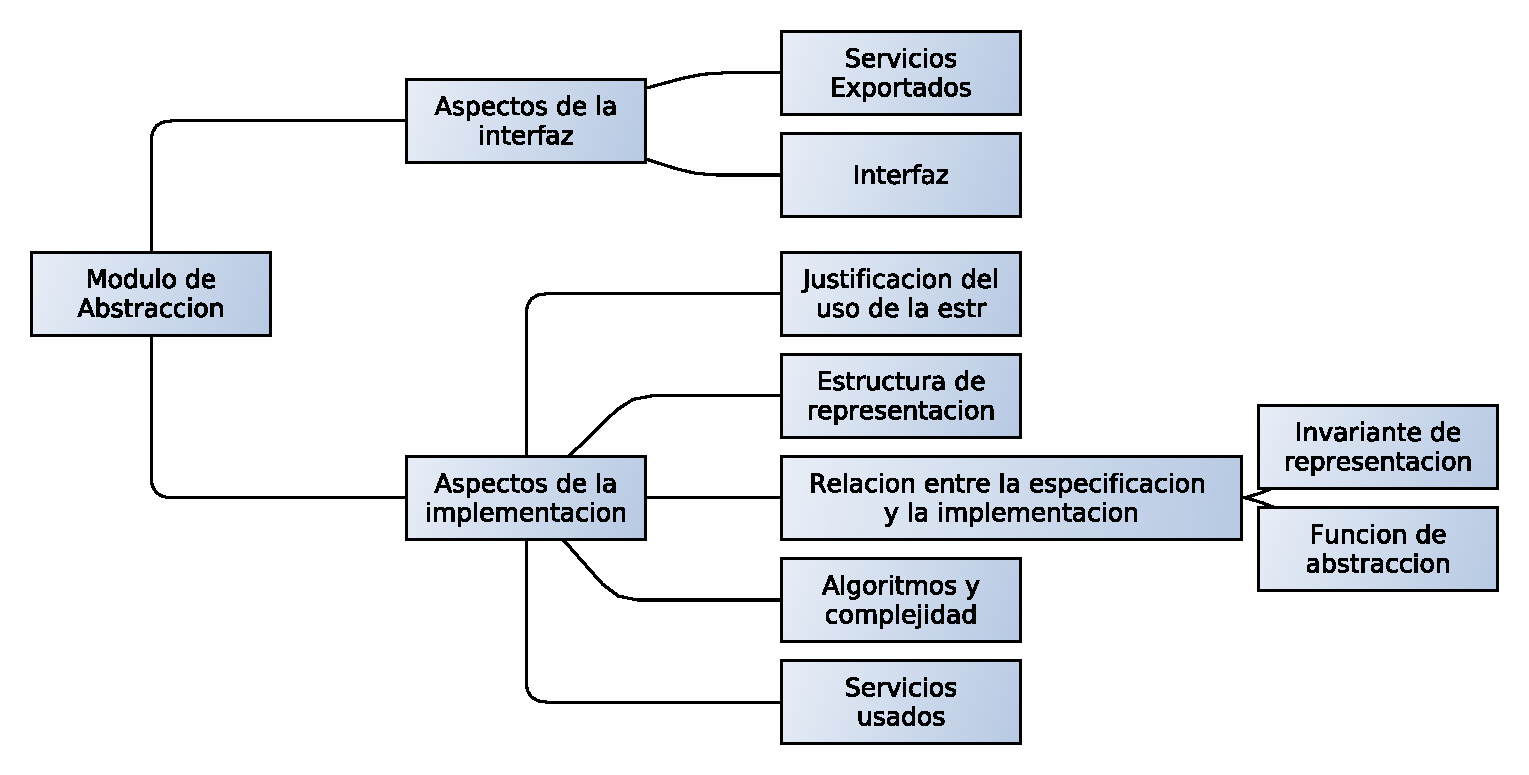
\includegraphics[width=0.7\textwidth]{ModuloDeDisenio.pdf}
\end{SCfigure}

\begin{itemize}
 \item \textbf{Especificaci\'on} Puede omitirse si es uno de los TADs provistos por la c\'atedra, o incluirse s\'olo los cambios si es una extensi\'on de un TAD ya conocido.
 \item \textbf{Interfaz} La cual contendr\'a los servicios exportados, \'ordenes de complejidad, aspectos de alising, efectos secundarios, etc. En definitiva, todo lo que el usuario necesite saber.
 \item \textbf{Representaci\'on} Estructura interna, invariante, funci\'on de abstracci\'on y algoritmos.
 \item \textbf{Servicios usados} \'Ordenes de complejidad, aspectos de alising, etc. requeridos de los tipos de soporte que utilizamos en nuestro m\'odulo.
\end{itemize}


\subsection{Aspectos de la Interfaz}

En este paso tomamos las decisiones concernientes al cambio de paradigma. Una forma de lograr esto es redefinir las aridades de las funciones adapt\'andolas a un lenguaje imperativo explicitando los requerimientos (precondiciones) para la aplicaci\'on de cada operaci\'on y los efectos que tiene sobre el estado de la m\'aquina (postcondiciones). Para escribir las precondiciones y las postcondiciones usaremos un lenguaje de descripci\'on de estados aprovechando la especificaci\'on del tipo a dise\~nar.

~

Durante la redefinici\'on de aridades no debemos limitarnos a cambiar una operaci\'on por un procedimiento como as\'i tambi\'en a respetar exactamente la cantidad de par\'ametros que tiene una operaci\'on. Siempre podremos decidir usar m\'as de un procedimiento para reemplazar a una operaci\'on del tipo abstracto como as\'i tambi\'en, y contrariamente, tendremos la posibilidad de unir varias funciones del tipo abstracto en una sola del dise\~no. Adem\'as de poder evitar totalmente el mapeo uno a uno podremos incluir funciones que no tengan sentido desde el punto de vista abstracto pero sean \'utiles dentro del paradigma imperativo, por ejemplo funciones para copiar instancias del tipo o funciones como ``comprimir'' cuyos efectos sean visibles solo desde la eficiencia temporal y espacial de las operaciones, pero no signifiquen un cambio en el valor representado. Todas estas decisiones dependen del contexto de uso.

\subsubsection{Servicios exportados / Operaciones exportadas}

En esta secci\'on deben estar expresados los detalles acerca de nuestro m\'odulo que resulten indispensables a sus usuarios. Es imprescindible tocar temas como la complejidad temporal de los algoritmos y cuestiones de alising y efectos secundarios de las operaciones. Adem\'as, pueden exhibirse comentarios (a modo informativo) con respecto a la implementaci\'on del m\'odulo que, aunque tengan menor importancia, sean de inter\'es para el usuario. Los puntos a recalcar que debe tocar esta \'area son los siguientes:

\begin{itemize}
 \item Deducir y documentar la \textbf{complejidad temporal} de cada operaci\'on es fundamental dentro de esta area, ya que de no haber informaci\'on de la misma nuestro m\'odulo no podr\'ia ser utilizado por ning\'un otro m\'odulo cuyo contexto de uso restringiera tal aspecto. Dicho de otra forma, un usuario que deba responder a requerimientos de eficiencia temporal y deba usar nuestro m\'odulo, no podr\'a saber si esta cumpliendo con ellos si no documentamos los mismos.
 \item Conocimiento del \textbf{alising} es de vital importancia para el uso correcto y eficiente del m\'odulo. Si no inform\'asemos las cuestiones de alising referentes a las operaciones podr\'ia pasar que un usuario de nuestro m\'odulo modifique datos sin saberlo por estar utilizando alg\'un alias (en vez de una copia) generado a partir del uso de de una de nuestras operaciones, lo que provocar\'ia un problema muy grave en el desarrollo del programa.
 \item Es importante indicar en las operaciones que \textbf{eliminan elementos de la estructura} si dichos elementos seguir\'an existiendo o ser\'an eliminados. Esto afecta a los usuarios que tengan referencias a dichos elementos. Si se los elimina, las referencias a ellos dejar\'an de ser v\'alidas, en caso contrario seguir\'an vigentes pero ya no estar\'an en la estructura, por lo que ser\'a el usuario el encargado de liberarlas al momento de implementar su m\'odulo ya que de no hacerlo podr\'a producir una potencial perdida de memoria.
\end{itemize}

\subsubsection{Contexto de uso y requerimientos de eficiencia de los servicios prestados}

Como dijimos al inicio, el contexto de uso esta dado por el entorno en donde vaya a ser usado el programa del cual se derivar\'an, a trav\'es de un an\'alisis de las funciones que ser\'an m\'as usadas, los requerimientos de eficiencia y adem\'as que estructuras de datos que se ajustan mejor al contexto en el que se encuentra el dise\~no. No se puede conocer si un dise\~no es adecuado si no se aclara precisamente el contexto de uso. La idea es que la principal justificaci\'on para el resultado obtenido en cada iteraci\'on de dise\~no es el contexto de uso que se le impuso al dise\~nador.

\subsection{Aspectos de la Implementaci\'on}

El objetivo de esta secci\'on es definir la forma en que representaremos el tipo que estamos dise\~nando en esta iteraci\'on (o nivel). La elecci\'on de una forma de representaci\'on est\'a dada por la elecci\'on de una o m\'as estructuras, las cuales deber\'an estar debidamente justificadas. Adem\'as de elegir la estructura de representaci\'on, es necesario definir cu\'al es la relaci\'on entre la estructura de representaci\'on y el tipo representado. Por \'ultimo, se deber\'an proveer los algoritmos que operan sobre la estructura y que resuelven cada una de las operaciones.

La estructura de representaci\'on de las instancias de los tipos s\'olo ser\'a accesible (modificable, consultable) a trav\'es de las operaciones que se hayan detallado en la interfaz del m\'odulo de abstracci\'on respectivo. Las operaciones no exportadas tambi\'en tendr\'an acceso a esta informaci\'on, pero s\'olo podr\'an ser invocadas desde operaciones del mismo m\'odulo, es decir la visibilidad de las mismas fuera del m\'odulo ser\'a nula.

\subsubsection{Elecci\'on de la estructura de representaci\'on} %Relacionado con Contexto de uso y requerimientos de eficiencia de los servicios prestados, hay que unificar.

La elecci\'on de la estructura esta fundamentada sobre las operaciones que nos interesa optimizar y el contexto de uso en el que ser\'an utilizadas. No solo tomamos en cuenta la complejidad temporal para definir un criterio de optimizaci\'on sino que tambi\'en tomamos en cuenta el espacio de disco, espacio en memoria, reusabilidad, claridad, sencillez de la implementaci\'on, homogeneidad de los algoritmos, entre otros.

Las variables en un programa referencias valores. Ser\'a imposible el acceso a la representaci\'on interna de \'estos y esto redundar\'a en la modularidad de nuestro dise\~no y en el ocultamiento de la informaci\'on. El ocultamiento nos permite hacer invisibles algunos aspectos que ser\'an encapsulados. Esto es \'util para aumentar el nivel de abstracci\'on y dise\~nar c\'odigo que sea m\'as f\'acilmente modificable, mantenible y extensible. Al acceder a los objetos s\'olo a trav\'es de su interfaz no nos atamos a su implementaci\'on, s\'olo a su funcionalidad. Cualquier cambio de implementaci\'on en un tipo que no altere la funcionalidad no nos obligar\'a a redise\~nar los tipos superiores.

\subsubsection{Relaci\'on entre la implementaci\'on y la abstracci\'on}

Para poder relacionar el mundo de los TADs con el mundo del dise\~no haremos uso de dos funciones que nos facilitaran esta tarea. Ambas funciones tendr\'an su dominio en las instancias de representaci\'on, estas son todas las formas que tendremos de instanciar la estructura de datos que elegimos en la representaci\'on sin restricci\'on alguna. Como podremos imaginar, muchas de estas formas de instancias la representaci\'on no tendr\'an sentido alguno para el tipo que estamos representando, mas que nada si las variables de nuestra representaci\'on tienen alguna correlaci\'on (por ejemplo, cantidad de elementos y la lista con dichos elementos), es aqu\'i en donde \textbf{invariante de representaci\'on} cobrar\'a importancia, ya que es el que nos indicara que instancias de la representaci\'on tienen sentido para el tipo abstracto que estamos representando y cuales no. Luego, la \textbf{funci\'on de abstracci\'on} servir\'a para llevar una instancia de representaci\'on al mundo de los TADs, es decir a una 
instancia del tipo abstracto de datos que estamos representando.

\subsubsection{Invariante de representaci\'on}

\begin{equation*}
Rep: \widehat{\text{genero\_de\_representacion}} \rightarrow boolean
\end{equation*}

El invariante de representaci\'on es un predicado que nos indica si una instancia de la estructura de representaci\'on es v\'alida para representar una instancia del tipo representado. De cierta forma, es el conocimiento sobre la estructura que necesitan las distintas operaciones para funcionar correctamente y que garantizan las mismas al finalizar su ejecuci\'on. Adem\'as funciona como un concepto coordinador entre las operaciones. En \'el quedan expresados las restricciones de coherencia de la estructura, surgidas de la redundancia de informaci\'on que pueda haber. Su dominio es la imagen funcional del tipo que estamos implementando, lo cual es necesario para que podamos ``tratar'' los elementos del dominio en l\'ogica de primer orden.

El invariante debe ser cierto tanto al comienzo de las \textbf{operaciones exportadas} del tipo como al final de las mismas. Por lo tanto, las operaciones del tipo deber\'an preservarlo, aunque quiz\'as no sea cierto en alg\'un estado intermedio del algoritmo que implemente alguna operaci\'on. Las \textbf{operaciones auxiliares} o internas, es decir aquellas que no aparecen en la interfaz y por lo tanto son invisibles a factores externos del m\'odulo, no tienen la necesidad conservar el invariante, sera de nuestra responsabilidad conocer que modificaciones le realizan a la estructura interna (de hacerlas) para luego restaurar el invariante.

De cierta forma, el invariante de representaci\'on fuerza a las operaciones a cumplir ciertos ordenes de complejidad y a preservar la coherencia en la estructura de representaci\'on. Adem\'as al ser un predicado que debe cumplirse gran parte del tiempo, podremos deducir propiedades del mismo que podremos usar como parte de nuestras demostraciones de correctitud y complejidad.

\subsubsection{Funci\'on de abstracci\'on}

\begin{equation*}
 Abs: \widehat{\text{genero\_de\_representacion}}\ g \rightarrow \widehat{\text{genero\_del\_tipo\_abstracto\_representado}} \ \ \ \ \{Rep(g)\}
\end{equation*}

La funci\'on de abstracci\'on es una herramienta que permite vincular una estructura de representaci\'on con el valor abstracto al que representa, es decir con el TAD vinculado al m\'odulo de abstracci\'on. Tiene por dominio al conjunto de instancias que son la imagen abstracta del tipo de representaci\'on (al igual que el invariante de representaci\'on) y que adem\'as verifican el invariante de representaci\'on, por esto mismo la funci\'on sera sobreyectiva. La funci\'on devuelve una imagen abstracta de la instancia del tipo representado (aquella instancia que estamos pretendiendo representar del tipo abstracto) y diremos que $T$ representa a $A$ si $Abs(\widehat{T})=_{obs} A$, en donde $T$ es una instancia de la representaci\'on y $A$ una instancia del TAD. Informalmente la funci\'on de abstracci\'on cumple la funci\'on de verificar que las funciones que alteran la estructura de representaci\'on realicen lo que est\'a especificado en el TAD y no otra cosa.

\begin{SCfigure}[1][ht!]
 \centering
 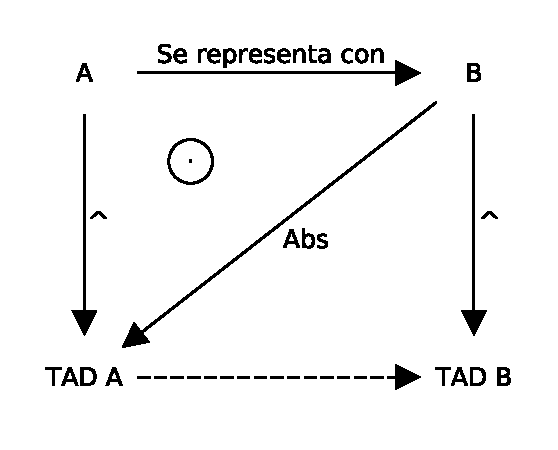
\includegraphics[width=0.3\textwidth]{FuncionDeAbstraccion.pdf}
 \caption*{\footnotesize $A$ ser\'a el modulo en cuesti\'on que estaremos dise\~nando y $B$ la estructura de representaci\'on del mismo. El circulo con el punto dentro hace alusi\'on al hecho de que la conmutaci\'on del triangulo conserva la sanidad. Esto significa que la aplicaci\'on de la funci\'on de abstracci\'on a $B$ deber\'a dar el mismo resultado que la aplicaci\'on de $\widehat{\text{\textbullet}}$ a $A$.
 \newline 
 \newline }
\end{SCfigure}

Tendremos dos formas de describir la funci\'on de abstracci\'on. La primera de ellas, en funci\'on de sus observadores b\'asicos. Dado que los observadores identifican de manera un\'ivoca al objeto del cual hablan, si nosotros describimos el valor que tienen los observadores b\'asicos una vez aplicados al objeto, estaremos describiendo desde un punto observacional pero sin ambig\"uedad el objeto representado. Otra forma de describir la funci\'on de abstracci\'on es utilizando los generadores del tipo de representaci\'on. La elecci\'on de elegir una forma u otra de hacerlo depende de la comodidad y declaratividad.

Dicho de otra forma, el objetivo de la funci\'on de abstracci\'on es poner en consonancia el tipo de soporte del modulo abstracto con los observadores del tipo que esta siendo representado. Una de las formas de realizar esto es caracterizando el valor de todos los observadores del TAD en base a valores de la instancia de la estructura de representaci\'on, de esa forma obtiene una instancia del TAD en consonancia con el modulo abstracto.

\subsubsection{Algoritmos}

En este paso se implementar\'an las operaciones del tipo a dise\~nar en t\'erminos de operaciones de los tipos soporte. Deben aparecer los algoritmos de cada una de las operaciones, sean \'estas de la interfaz o auxiliares. En el caso de las funciones auxiliares, es recomendable incluir junto a sus algoritmos, sus precondiciones y postcondiciones. En el dise\~no de los algoritmos hay que tener en cuenta que las operaciones deben satisfaces sus pre/postcondiciones, y adem\'as deben satisfacer los requerimientos de eficiencia surgidos en el contexto de uso.

\subsubsection{Servicios usados}

Aqu\'i es donde indicaremos qu\'e responsabilidades le dejamos a los tipos soporte que usamos. Son las pautas y requerimientos que se extraen del dise\~no de este tipo para el dise\~no de los tipos de la representaci\'on. Luego pasar\'an a ser las interfaces y los contextos de uso y requerimientos de eficiencia para los m\'odulos de soporte de los tipos usados en la representaci\'on.

\newpage

\chapter{Complejidad y Estructuras de Datos}

\section{Complejidad}
\subsection{Notaci\'on asint\'otica}

Las notaciones que usamos para describir la complejidad temporal asint\'otica de un algoritmo est\'an definidos en t\'erminos de funciones cuyos dominios son el conjunto de los n\'umeros naturales $N = \{0,1,2,...\}$. Estas notaciones son convenientes para describir el tiempo en el peor caso de una funci\'on $T(n)$, la cual usualmente esta definida solo en tama\~nos de entrada enteros. Sin embargo a veces encontramos conveniente abusar de la notaci\'on asint\'otica en variadas formas. De todas formas, deberemos cerciorarnos de entender precisamente el significado de la notaci\'on, para que cuando hagamos abuso de la misma no estemos us\'andola de forma err\'onea. Usaremos la notaci\'on asint\'otica primariamente para describir los tiempos que insumen los algoritmos, sin embargo la notaci\'on asint\'otica aplica a funciones.

\subsubsection{Conjunto / Notaci\'on Asint\'otica $\Theta$}

Para una funci\'on $g(n)$ dada, notaremos a $\Theta(g(n))$ como el conjunto de funciones $f(n)$ que a partir de un numero $n_0 > 0$ sus valores pueden ser acotados entre $c_1g(n)$ y $c_2g(n)$ para alg\'un $c_1, c_2 \in \Re_{>0}$. Descripto formalmente quedar\'ia de la siguiente manera:

\begin{equation*}
 \Theta(g(n)) = \{ f(n) : (\exists\ c_1, c_2, n_0 \in \Re_{>0}) \ (\forall n\ |\ n_0 \leq n)\ 0 \leq c_1 \cdot g(n) \leq f(n) \leq c_2 \cdot g(n) \}
\end{equation*}

~

Una funci\'on pertenece al conjunto $\Theta(g(n))$ si existen constantes positivas $c_1$ y $c_2$ tal que $f(n)$ puede ser ``sandwicheada'' entre $c_1g(n)$ y $c_2g(n)$, para un $n$ suficientemente grande. Como $\Theta(g(n))$ es un conjunto, podremos escribir ``$f(n) \in \Theta(g(n))$'' para indicar que $f(n)$ es un miembro de $\Theta(g(n))$, a veces escribiremos ``$f(n) = \Theta(g(n))$'' para expresar exactamente lo mismo. Cuando una funci\'on $f(n)$ es acotada superiormente por otra funci\'on $c \cdot g(n)$ para alg\'un $c$ y a partir de alg\'un $n$, diremos que $f(n)$ esta \textbf{acotada asint\'oticamente} por $g(n)$ o que $f(n)$ tiene un \textbf{comportamiento asint\'otico} a $g(n)$. En el caso de $\Theta(g(n))$ diremos que $g(n)$ es una \textbf{cota asint\'oticamente ajustada} para $f(n)$.

\subsubsection{Conjunto / Notaci\'on Asint\'otica $O$}

El conjunto $\Theta$ asint\'oticamente acota una funci\'on inferior y superiormente. Cuando solo tenemos una \textbf{cota asint\'otica superior}, usaremos el conjunto $O$. Para una funci\'on dada $g(n)$, denotaremos por $O(g(n))$ al conjunto de funciones tales que:

\begin{equation*}
 O(g(n)) = \{ f(n) : (\exists\ c, n_0 \in \Re_{>0}) \ (\forall n\ |\ n_0 \leq n)\ 0 \leq f(n) \leq c \cdot g(n) \}
\end{equation*}

~

Es decir que para todos los valores de $n$ a la derecha de $n_0$, el valor de la funci\'on $f(n)$ es o esta por debajo de $c \cdot g(n)$. Escribiremos $f(n) = O(g(n))$ para indicar que una funci\'on $f(n)$ es un miembro del set $O(g(n))$. Notar que $f(n) = \Theta(g(n))$ implica $f(n) = O(g(n))$, ya que la noci\'on de $\Theta$ es mucho mas fuerte que la noci\'on de $O$. Esto es, escrito en forma de teor\'ia de conjuntos, que vale la inclusi\'on $\Theta(g(n)) \subseteq O(g(n))$

\subsubsection{Conjunto / Notaci\'on Asint\'otica $\Omega$}

De forma tal como la notaci\'on $O$ proporciona una cota asint\'otica en una funci\'on, $\Omega$ provee una \textbf{cota asint\'otica inferior}. Para una funci\'on dada $g(n)$, notaremos a $\Omega(g(n))$ como el conjunto de funciones tales que:

\begin{equation*}
 \Omega(g(n)) = \{ f(n) : (\exists\ c n_0 \in \Re_{>0}) \ (\forall n\ |\ n_0 \leq n)\ 0 \leq c \cdot g(n) \leq f(n) \}
\end{equation*}

~

Cuando decimos que el tiempo de un algoritmo es $\Omega(g(n))$, significa que no importa que particular entrada de tama\~no $n$ para cada valor de $n$, el tiempo que tardara el algoritmo con dicha entrara sera de al menos un numero constante de veces $g(n)$, para un $n$ suficientemente grande. Equivalentemente, esto nos da una cota temporal inferior para el mejor caso del algoritmo. De las definiciones de las notaciones asint\'oticas, es f\'acil ver que para cualquier dos funciones $f(n)$ y $g(n)$, tendremos que $f(n) = \Theta(g(n))$ si y solo si $f(n) = O(g(n))$ y $f(n) = \Omega(g(n))$. Usando una notaci\'on de teor\'ia de conjuntos esto seria equivalente a decir que $\Omega(g(n)) \cap O(g(n)) = \Theta(g(n))$, y si $f(n) \in \Omega(g(n)) \land f \in O(g(n))$ entonces $f(n)$ pertenecer\'a a ambos conjuntos, por lo que en particular pertenecer\'a a la intersecci\'on $\Theta(g(n))$.

\subsubsection{Conjunto / Notaci\'on Asint\'otica No-Ajustada $o$}

La cota superior asint\'otica provista por $O$ puede o no puede ser ajustada asint\'oticamente, pero la cota $2n = O(n^2)$ no lo es. Usaremos la notaci\'on $o$ (o chica) para definir una cota superior que no sea ajustada asint\'oticamente. Para una funci\'on dada $g(n)$, definiremos formalmente a $o(g(n))$ como el conjunto de funciones tales que:

\begin{equation*}
 o(g(n)) = \{ f(n) : (\exists\ c, n_0 \in \Re_{>0}) \ (\forall n\ |\ n_0 \leq n)\ 0 \leq f(n) < c \cdot g(n) \}
\end{equation*}

~

Las definiciones de $O$ (o grande) y $o$ (o chica) son sumamente similares. La diferencia principal yace en que $f(n) = O(g(n))$, la cota $0 \leq f(n) \leq c \cdot g(n)$ se mantiene para alguna constante $c > 0$ mientras que en $f(n) = o(n)$, la cota $0 \leq f(n) < c \cdot g(n)$ se mantiene para todas las constantes $c > 0$. Intuitivamente, en la notaci\'on $o$, la funci\'on $f(n)$ se vuelve asint\'oticamente parecida a $g(n)$ a medida que $n$ tiende a infinito.

\subsubsection{Conjunto / Notaci\'on Asint\'otica No-Ajustada $\omega$}

Anal\'ogicamente, $\omega$ es a $\Omega$ como $o$ es a $O$. Usaremos la notaci\'on $\omega$ para referirnos a una cota inferior que no sea ajustada asint\'oticamente. Una forma de definirla en funci\'on a $o$ sera que $f(n) \in \omega(g(n))$ si y solo si $g(n) \in o(f(n))$. De todas formas formalmente definiremos a $\omega$ como el conjunto de funciones tal que dada una funci\'on $g(n)$ es:

\begin{equation*}
 \omega(g(n)) = \{ f(n) : (\exists\ c n_0 \in \Re_{>0}) \ (\forall n\ |\ n_0 \leq n)\ 0 \leq c \cdot g(n) < f(n) \}
\end{equation*}

~

A medida que $n$ tiende a infinito la relaci\'on entre $f(n)/g(n)$ se vuelve arbitrariamente grande, es decir que tiende a infinito.

\newpage
\section{Estructuras b\'asicas}
\subsection{Lista}
\subsection{Cola}
\subsection{Pila}
\subsection{Arreglo dimensionable}

\newpage
\section{\'Arboles}
\subsection{\'Arbol binario de b\'usqueda}

Un \'arbol binario de b\'usqueda es un \'arbol basado en nodos binarios el cual puede ser representado por una estructura de punteros en donde cada nodo es un objeto. En adici\'on a la clave y a los datos, cada nodo contiene los atributos izquierda, derecha y p, los cuales son punteros que apuntan a su hijo izquierdo, hijo derecho y padre, respectivamente. Si un hijo o un padre esta perdido el atributo apropiado contiene el valor $NIL$. El nodo ra\'iz es el \'unico nodo cuyo padre es $NIL$.

Las claves en un \'arbol binario de b\'usqueda siempre est\'an guardadas de forma tal de satisfacer la \textbf{invariante del \'arbol binario de b\'usqueda}, el cual se define como: ''Sea $x$ un nodo en un \'arbol de b\'usqueda binario. Si $y$ es un nodo en el sub-\'arbol izquierdo de $x$, entonces $y.clave \leq x.clave$. Si $y$ es un nodo en el sub-\'arbol derecho de $x$, entonces $y.clave \geq x.clave$``

\subsubsection{B\'usqueda}

La b\'usqueda en un \'arbol binario se logra utilizando el invariante presentado anteriormente. El procedimiento comienza en la ra\'iz y por cada nodo $x$ que encuentra compara la clave $k$ con $x.clave$, si las dos claves son iguales, la b\'usqueda termina. Si $k$ es mas chico que $x.clave$, la b\'usqueda continua por el sub-\'arbol izquierdo de $x$, dado que el invariante del \'arbol binario de b\'usqueda implica que $k$ no puede ser guardado en el sub-\'arbol derecho. Sim\'etricamente, si $k$ es mas grande que $x.clave$, la b\'usqueda continua por el sub-\'arbol derecho. Los nodos encontrados durante la recursion forman un camino simple desde la ra\'iz, por lo que el tiempo de corrida de una b\'usqueda en un \'arbol binario es de $O(h)$, en donde $h$ es la altura del \'arbol la cual puede ser $n$ si tenemos un \'arbol totalmente degenerado, que de cierta forma terminar\'ia siendo una lista enlazada.

Adem\'as, siempre podremos encontrar un elemento en un \'arbol binario cuya clave sea un m\'inimo o un m\'aximo siguiendo los punteros izquierdos o derechos desde la ra\'iz hasta que encontremos un $NIL$.

\subsubsection{Inserci\'on}

Las operaciones de inserci\'on y borrado causa que la din\'amica del conjunto representado por un \'arbol binario de b\'usqueda cambie. La estructura de datos debe ser modificada para reflejar este cambio, pero de forma tal que el invariante se conserve.

Para insertar un nuevo valor $v$ en un \'arbol binario de b\'usqueda $T$, crearemos un nuevo nodo $z$ de tal forma que $z.clave = v$, $z.izq = NIL$ y $z.der = NIL$. Modificara $T$ y alguno de los atributos de $z$ de tal forma que inserte $z$ en la posici\'on apropiada del \'arbol. Para lograr insertar el nuevo nodo el procedimiento guardar\'a en una variable $p$ un puntero al nodo actual en donde se encuentra mientras que ejecuta una b\'usqueda en el \'arbol. Una vez que llega a un nodo NIL durante la b\'usqueda, asigna $z.p = p$ y compara $z.clave$ con $p.clave$, si es mayor asigna $p.izq = z$ y si es menor $p.der = z$, de esta forma el invariante queda restaurado. El tiempo de esta operaci\'on se encontrara en el orden de $O(h)$, siendo que $h$ puede ser $n$ en el peor caso el tiempo ser\'a de $O(n)$, sin embargo el caso promedio suponiendo una distribuci\'on uniforme en la entrada de los valores sera de $O(lg(n))$.

\subsubsection{Borrado}

La estrategia general para eliminar un nodo $z$ de un \'arbol binario de b\'usqueda $T$ tiene $3$ casos b\'asicos, pero como veremos uno de ellos es algo enga\~noso.

\begin{itemize}
 \item Si $z$ no tiene hijos, entonces simplemente lo removeremos modificando su padre $z.p$ reemplazando el puntero a $z$ por $NIL$.
 \item Si $z$ solo tiene un hijo, entonces \textbf{elevaremos} dicho hijo para tomar la posici\'on de $z$ modificando el padre $z.p$ reemplazando el puntero a $z$ por el puntero al \'unico hijo de $z$.
 \item Si $z$ tiene dos hijos, entonces encontraremos el m\'inimo $y$ en el sub-\'arbol derecho de $z$ (es decir, su sucesor), para tomar la posici\'on de $z$ en el \'arbol. Como $y$ era el m\'inimo del sub-\'arbol derecho de $z$, $y.izq$ sera $NIL$ y si $y$ tiene un hijo izquierdo lo elevaremos al padre de $y$. Luego, con $y$ libre hijos, lo reemplazaremos por $z$ y le asignaremos los sub-\'arboles derecho e izquierdo, como hijos de $y$. Esto mismo se puede hacer si tomamos como $y$ el m\'aximo del sub-\'arbol izquierdo de $z$.
\end{itemize}

%TODO: Factor de Balanceo.

\subsubsection{Rotaciones}

Las rotaciones son operaciones locales en un \'arbol de b\'usqueda que cambian la estructura de punteros del mismo preservando el invariante del \'arbol binario, son mayormente usadas en las distintas implementaciones de \'arboles balanceados para ajustar los factores de balanceo del mismo. Usaremos dos tipos de rotaciones, rotaciones hacia la izquierda y rotaciones hacia la derecha. Cuando hacemos una rotaci\'on hacia la izquierda en un nodo $x$, asumimos que su hijo derecho $y$ no es $NIL$; $x$ podr\'a ser cualquier nodo en el \'arbol cuyo hijo derecho no es $NIL$. La rotaci\'on hacia la izquierda ''pivotea`` alrededor del enlace de $x$ a $y$ y hace a $y$ la nueva ra\'iz del sub-\'arbol, dejando como hijo izquierdo de $y$ a $x$ y trasladando a el hijo izquierdo de $y$ al lugar del hijo derecho de $x$. 

\begin{SCfigure}[1][ht!]
 \centering
 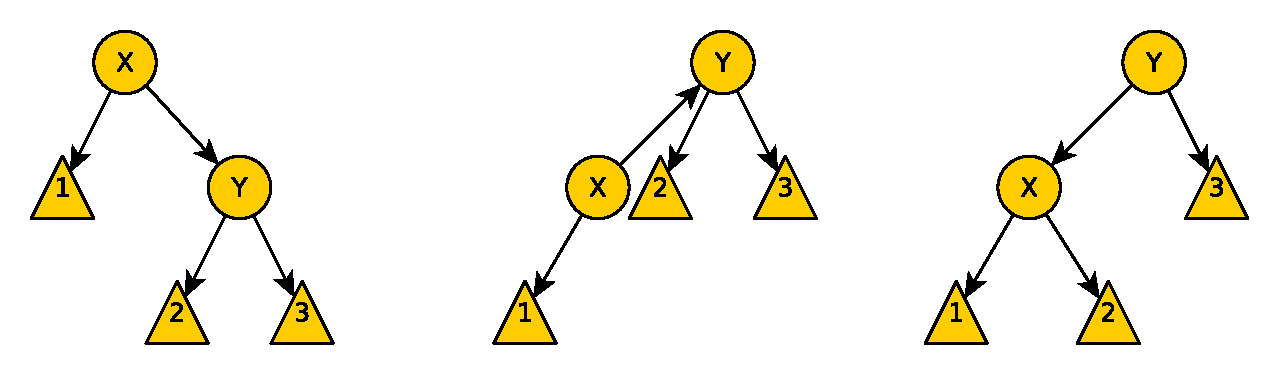
\includegraphics[width=0.7\textwidth]{RBRotacionIzq.pdf}
 \caption*{\newline \footnotesize Si nos imaginamos la rotaci\'on como bolillas e hilos, ''tirar\'iamos`` $y$ hacia arriba a la izquierda, haciendo que $x$ baje y quede a la altura del hijo izquierdo de $y$. Luego, como el hijo izquierdo de $y$ se encontraba en el sub-\'arbol derecho de $x$, sera mas grande que $x$, por lo que lo podremos asignar como hijo derecho de $x$.}
\end{SCfigure}


%Falta ver inorder

\subsubsection{Complejidades}

\begin{itemize}
 \item \textbf{B\'usqueda} $O(n)$ (caso promedio $O(lg(n))$)
 \item \textbf{Inserci\'on} $O(n)$ (caso promedio $O(lg(n))$)
 \item \textbf{Borrado} $O(n)$ (caso promedio $O(lg(n))$)
 \item \textbf{Espacio} $O(n)$
\end{itemize}

\subsection{Heap}

La estructura de datos del heap (binario) es un arreglo de objetos que podremos ver como un \'arbol binario casi-completo. Cada nodo del \'arbol corresponde a un elemento del arreglo y el \'arbol esta completamente lleno en todos los niveles excepto en el ultimo, el cual esta lleno desde la izquierda hasta alg\'un punto. Un arreglo $A$ que representa un heap es un objeto con dos atributos, $A.lenght$ que nos dir\'a la cantidad de elementos en el arreglo y $A.heap\_size$ que representara cuantos elementos en el heap est\'an guardados en el arreglo $A$. Esto es, que a pesar que $A[1..A.length]$ contenga n\'umeros, solo los elementos en $A[1..A.heap\_size]$ (en donde $0 \leq A.heap\_size \leq A.length$) son elementos validos del heap.

~

La ra\'iz del \'arbol estar\'a situada en $A[1]$, y dado el \'indice $i$ de un nodo, f\'acilmente podremos computar los \'indices de su padre, hijo derecho e izquierdo. Los c\'omputos del \'indice del padre estar\'a definido de la forma $Padre(i) = \lfloor i/2 \rfloor$, mientras que los \'indices de los hijos podr\'an ser computados de la forma $Izquierda(i) = 2i$ y $Derecha(i) = 2i+1$, en donde $i \in [1..A.heap\_size]$. Hay dos tipos de heaps binarios, max-heaps y min-heaps. En ambos casos, los valores de los nodos satisfacen el invariante del heap, el cual depende del tipo de heap con el que trabajemos. En un max-heap, el invariante del max-heap nos dice que para cada nodo $i$ que no sea la ra\'iz se debe cumplir que $A[Padre(i)] \geq A[i]$, esto es que el valor de un nodo debe ser como m\'aximo el valor de su padre. Entonces, el m\'aximo en un max-heap estar\'a guardado en la ra\'iz, y el sub-\'arbol con ra\'iz en un nodo no podr\'a contener valores mas grandes que el nodo en si mismo. Un min-heap esta 
organizado de la forma opuesta, el invariante de min-heap nos dice que para cada nodo $i$ distinto de la ra\'iz se debe cumplir $A[Padre(i)] \leq A[i]$, por lo que el elemento m\'inimo de un min-heap estar\'a en la ra\'iz.

~

Viendo el heap como un \'arbol, definiremos la altura de un nodo en un heap como el numero de aristas en el camino simple mas largo desde el nodo mismo hasta una hoja, y definiremos la altura del heap como la altura de su ra\'iz. Ya que un heap de $n$ elementos esta basado en un \'arbol binario completo, su altura pertenecer\'a a $\Theta(lg(n))$.

\subsubsection{Mantener el invariante del heap}

De aqui en mas, asumiremos que estaremos hablando de un max-heap, ya que el min-heap es an\'alogo. Para mantener el invariante del max-heap en un arreglo, llamaremos al procedimiento \textbf{Heapify}. Su entrada sera el arreglo $A$ y un \'indice $i$ del arreglo. Cuando es llamado, Heapify asume que los sub-\'arboles binarios con sus ra\'ices en $Izquierda(i)$ y $Derecha(i)$ ser\'an max-heaps, pero que $A[i]$ puede ser mas chico que que sus hijos, violando as\'i el invariante. Heapify deja que el valor en $A[i]$ ''decante`` en el max-heap, de forma tal que el sub-\'arbol con raiz en $i$ cumpla el invariante del heap y luego recursivamente se asegurara que el invariante sea cumplido en el sub-\'arbol en donde el valor $A[i]$ haya decantado.

~

Puntualmente lo que realiza Heapify es, estando situado en $i$, compara el valor con los valores de los hijos de $i$. Si ninguno de los valores de los hijos es mas grande que el valor de $i$ lo deja como esta, en el caso contrario intercambia el valor de $i$ con el valor de su hijo mas grande. Si bien en el nodo original el invariante se cumple, el invariante puede ser violado en el sub-\'arbol cuya ra\'iz fue intercambiada por lo que se realiza una llamada recursiva utilizando como $i$ el nuevo \'indice donde el valor fue intercambiado.

~

El tiempo de Heapify en un sub-\'arbol de tama\~no $n$ con su ra\'iz en un nodo $i$ sera el tiempo $\Theta(1)$ para ajustar las relaciones entre los elementos $A[i]$, $A[Izquierda(i)]$ y $A[Derecha(i)]$, mas el tiempo que tome correr Heapify en un sub-\'arbol con su ra\'iz en alguno de los hijos del nodo $i$ (asumiendo que la llamada recursiva ocurra). El peor caso ocurrir\'a cuando el nivel inferior del \'arbol se encuentre exactamente a la mitad de estar lleno, por lo que cada uno de los sub-\'arboles de los hijos tendr\'an como mucho $2n/3$ elementos. Podremos describir el tiempo de Heapify con la recurrencia $T(n) \leq T(2n/3) + \Theta(1)$. Si tuvi\'esemos $T(n) = T(2n/3) + \Theta(1)$, la recurrencia se ajusta al segundo caso del teorema maestro, por lo que $T(n) \subseteq \Theta(lg(n))$ pero como tenemos una relaci\'on de menor o igual en la recurrencia original, $T(n) \subset O(lg(n))$.

\subsubsection{Construyendo un heap}

Podremos usar el procedimiento Heapify de forma bottom-up para convertir un arreglo $A[1..n]$, en donde $n=A.length$, en un max-heap. Los elementos en el sub-arreglo $A[\lfloor n/2\rfloor + 1 .. n]$ son todas hojas del \'arbol, y por lo tanto cada uno es un heap de $1$ elemento por el cual podremos comenzar. El procedimiento para construir un heap va por cada uno de los nodos del \'arbol restantes comenzando por el \'indice mas grande, es decir $i = \lfloor A.length/2 \rfloor .. 1$, y ejecuta Heapify en cada uno de ellos. Una cota grosera para este procedimiento es $O(nlg(n))$, ya que har\'a $n$ llamadas a Heapify. Sin embargo, una cota mas ajustada puede ser dada bas\'andonos en que la altura de un \'arbol heap de $n$ elementos tiene altura $\lfloor lg(n) \rfloor$ y como mucho $\lceil n/2^{h+1}\rceil$ nodos de cualquier altura $h$, la cual corresponder\'a con $O(n)$.

%TODO: Dar la demostracion de esto. Pagina 157 del cormen.

\subsubsection{Extraccion de m\'aximo e inserci\'on}

El m\'aximo en un max-heap sera $A[1]$, el cual una vez extra\'ido no ser\'a eliminado del arreglo sino que ser\'a intercambiado por el ultimo elemento del arreglo y luego se decrementara $A.heap\_size$ en una unidad, dejando fuera del scope al ultimo elemento del arreglo que ser\'a aquel que acabamos de extraer. El \'unico problema con esto es que estaremos rompiendo el invariante del heap, pero para solucionarlo solo nos bastara con aplicar $Heapify(A,1)$ ya que el resto de los sub-heaps seguir\'an siendo validos. Como todas las operaciones son $\Theta(1)$ exceptuando Heapify, la cual se usar\'a una sola vez, el tiempo total del algoritmo sera de $O(lg(n))$.

%TODO: Pseudocodigo de extraccion, pagina 163 del cormen

~

Para insertar un nuevo elemento incrementaremos la variable $A.heap\_size$ en una unidad y asignaremos el nuevo valor a la ultima posici\'on valida para el heap, es decir $A[heap\_size] = valor$. Luego, intercambiaremos su valor con el padre hasta que el invariante del heap se cumpla.

%TODO: Pseudocodigo de inserci\'on, pagina 164 del cormen.

\subsubsection{En resumen}

Los heaps son \'arboles balanceados en donde la clave de cada nodo es mayor o igual que la de sus hijos y en donde todo sub-\'arbol es un heap. Adicionalmente puede o no cumple que por la forma de su implementaci\'on sea izquierdista, esto quiere decir que el \'arbol estar\'a todo lleno exceptuando su ultimo nivel, el cual se llenara de izquierda a derecha.

Su representaci\'on podr\'a estar dada por cualquier tipo de estructura para \'arboles binarios, pero si bien sera mas eficiente si se lo representa en un arreglo, pasaremos a una representaci\'on est\'atica por lo que podremos perder tiempo agrandando un arreglo. Sea un nodo $v$, la posici\'on dentro de un heap se calcula:

\begin{itemize}
 \item Si $v$ es la ra\'iz, $P(v) = 1$
 \item Si $v$ es un nodo que no es la ra\'iz, su padre $u$ sera $P(v) = \lfloor P(u)/2\rfloor$. Sea $i$ un \'indice de un nodo: $Padre(i) = \lfloor i/2\rfloor$.
 \item Si $v$ es un hijo izquierdo de $u$ $P(v) = 2P(u)$. Sea $i$ un \'indice de un nodo: $Derecho(i) = 2i$.
 \item Si $v$ es un hijo derecho de $u$ $P(v) = 2P(v)+1$. Sea $i$ un \'indice de un nodo: $Izquierdo(i) = 2i+1$.
\end{itemize}

\subsubsection{Complejidades}
Las complejidades de las operaciones del heap quedaran de la forma:

\begin{itemize}
 \item \textbf{Ver el m\'aximo o m\'inimo / Pr\'oximo} $O(1)$
 \item \textbf{Extraer el m\'aximo o m\'inimo / Desencolar} $O(lg(n))$
 \item \textbf{Ingresar nuevo elemento / Encolar} $O(lg(n))$
 \item \textbf{Construir heap a partir de arreglo / Heapify} $O(n)$
\end{itemize}

\subsection{\'Arbol balanceado en altura (AVL)}

Un \'arbol AVL es un \'arbol binario de b\'usqueda que esta balanceado en altura. Esto es, que por cada nodo $x$, la altura de de los sub-\'arboles izquierdo y derecho de $x$ difieren en a lo sumo $1$. Para implementar un \'arbol AVL mantendremos un atributo extra en cada nodo $x.fdb$ que representara el factor de balanceo del nodo $x$. El factor de balanceo para un nodo $x$ se calculara de la forma $FDB(x) = altura(der(x)) - altura(izq(x))$.

\subsubsection{Inserci\'on}

La inserci\'on de un nuevo nodo en un principio se realiza de la misma manera que en un ABB normal. Luego de haber insertado el nodo se realizan dos acciones:

\begin{itemize}
 \item Se recalculan los factores de balanceo de forma bottom-up, es decir comenzando por el nodo reci\'en insertado hasta la ra\'iz. Esto funciona ya que los factores de balanceo de otros nodos que no pertenezcan a la rama del nodo reci\'en insertados no se ver\'an afectados por la inserci\'on.
 \item Si durante el recalculo aparece un factor $\pm 2$ en alguno de los pasos, habr\'a que rebalancear el nodo antes de continuar.
\end{itemize}

Durante el rebalanceo de un nodo aparecer\'an distintos casos para los cuales deberemos aplicar distintas rotaciones. La notaci\'on de cada uno de los casos va de la forma $D_1D_2$, siendo $x$ el nodo que necesitamos rebalancear $D_2$ indicar\'a el hijo de $x$ en cuyo sub-\'arbol $D_1$ fue hecha la inserci\'on del nuevo elemento. Es decir, si tenemos un caso $RL$, significa que estando parados en un nodo $x$ la inserci\'on fue hecha en el sub-\'arbol derecho del hijo izquierdo de $x$. De cierta forma la notaci\'on se traduce desde abajo hacia arriba en un \'arbol.

~

Estos casos son $LL$ y $RR$, a los cuales ser\'a suficiente con aplicarles rotaciones simples para solucionarlos y $LR$ y $RL$ a los cuales habr\'a que aplicarles una rotaci\'on para dejarlos en alguno de los casos anteriores y una segunda rotaci\'on para terminar de balancearlos. Tanto $LL$ a $RR$ y $LR$ a $RL$ son casos sim\'etricos unos de otros.

~

\begin{SCfigure}[1][ht!]
 \centering
 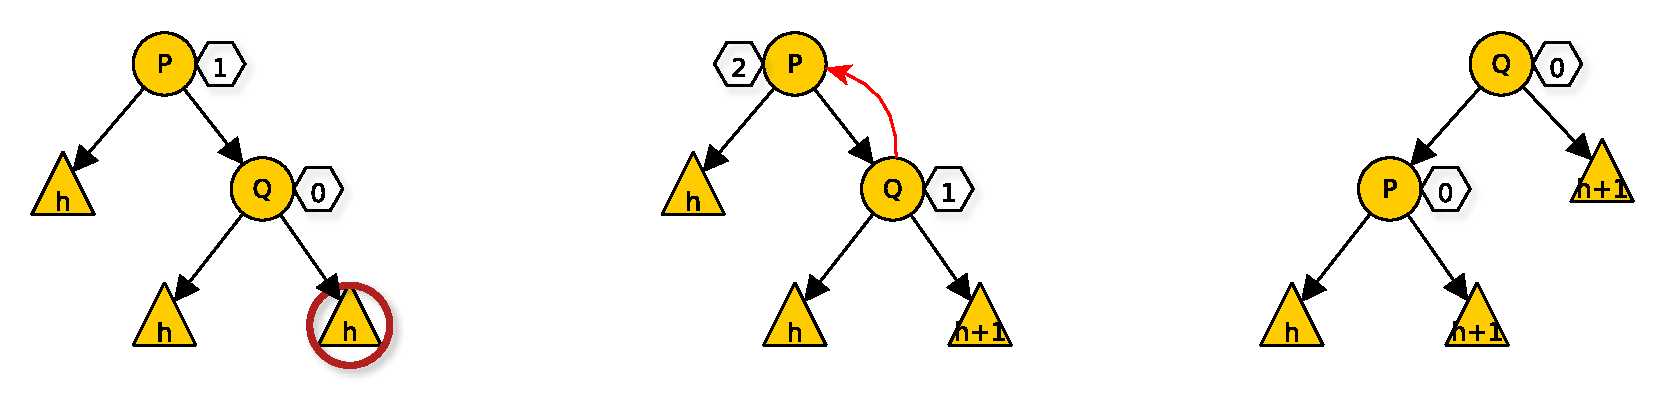
\includegraphics[width=0.70\textwidth]{RotacionSimpleAVL.pdf}
 \caption*{\newline \footnotesize \textbf{Caso RR} En la primera figura se observa el estado inicial, dentro de los hex\'agonos se encuentra el FDB de cada nodo. En la segunda figura se puede observar el estado luego de la inserci\'on y FDB desbalanceado del nodo $P$. Ejecutando una rotaci\'on hacia la izquierda entre $P$ y $Q$ se restaura, como se ve en la tercera figura. El caso $LL$ es sim\'etrico a este caso.}
\end{SCfigure}

\newpage
\begin{SCfigure}[1][ht!]
 \centering
 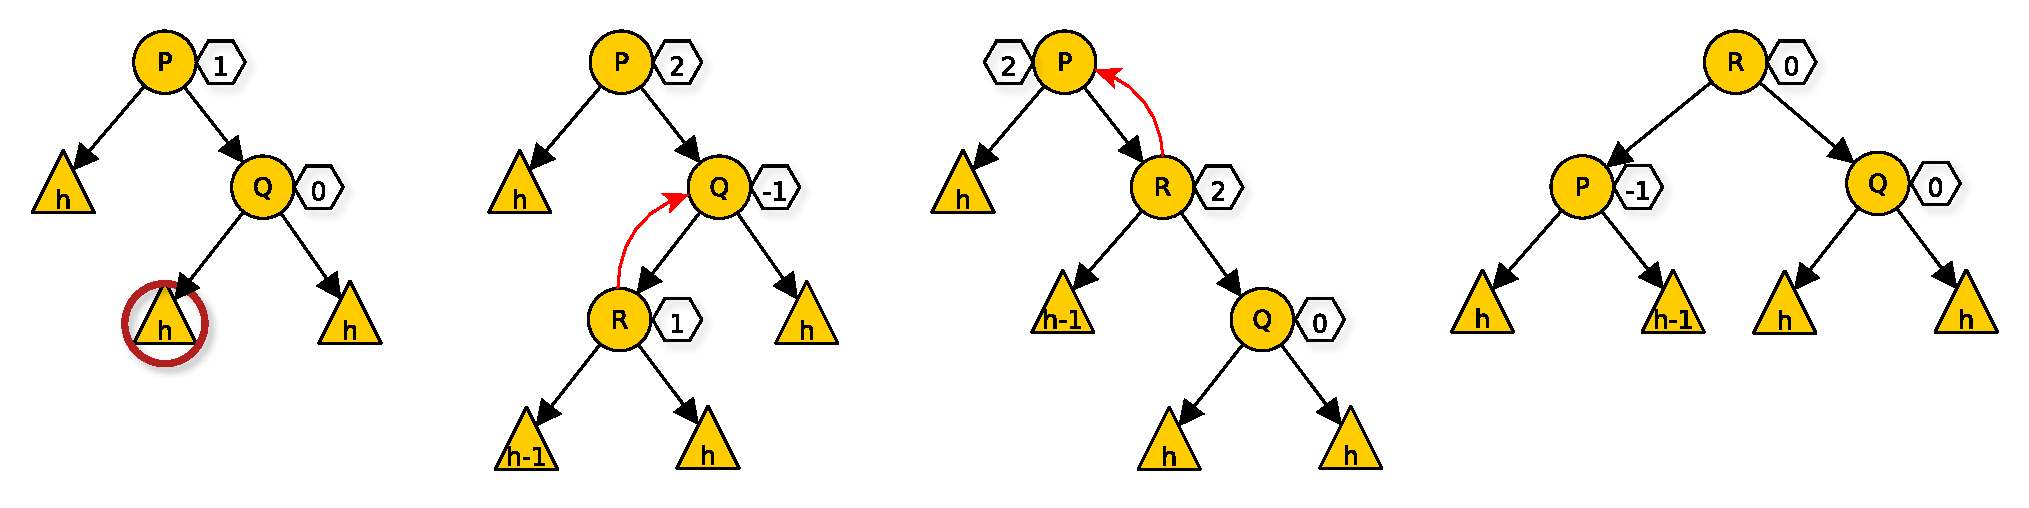
\includegraphics[width=0.70\textwidth]{RotacionDobleAVL.pdf}
 \caption*{\newline \footnotesize \textbf{Caso LR} En la primera figura se observa el estado inicial. En la segunda figura se puede observar el estado luego de la inserci\'on con el hijo izquierdo $R$ de $Q$ expandido, la primera rotaci\'on se ejecutar\'a hacia la derecha entre $R$ y $Q$. La tercer figura refleja el estado luego de la primer rotaci\'on, en este estado se ejecutara la segunda rotaci\'on que ser\'a hacia la izquierda entre $P$ y $R$. La cuarta figura refleja el estado final con el nodo balanceado. El caso $RL$ es sim\'etrico a este caso.}
\end{SCfigure}

~

La rotaciones en el caso de inserci\'on no influyen en los antepasados de $x$, por lo que su balance no ser\'a modificado, y por lo tanto a lo sumo necesitaremos realizar dos rotaciones para rebalancear el \'arbol luego de una inserci\'on. El tiempo que tomara entonces una inserci\'on sera $O(2lg(n)) \subseteq O(lg(n))$, ya que deberemos buscar el lugar para insertar el nodo y luego recalcular todos los factores de balanceo de la rama (de ser necesario se rebalancear\'a alguno de los nodos).

\subsubsection{Eliminaci\'on}

El borrado en un AVL en un principio se realiza de la misma forma que en un \'arbol binario, luego de haberlo hecho se ejecuta un recalculo de los factores y un rebalanceo sobre la rama que se vio afectada por el mismo. Una diferencia importante entre la inserci\'on y el borrado es que a la hora de realizar los rebalanceos en la inserci\'on los antepasados de un nodo $x$ desbalanceado no se ver\'an influenciados mientras que durante un rebalanceo luego de un borrado si lo har\'an. 

~

Esto \'ultimo se debe a que durante la inserci\'on estaremos agregando una hoja nueva, y por la naturaleza del AVL el balanceo de un sub-\'arbol $T$ con su raiz en $x$ ocasiona que la altura de $T$ se acorte. Esto significa que de cierta forma mediante el balanceo estaremos cancelando el incremento de altura en el sub-\'arbol $T$ ocasionado por la inserci\'on, por lo que los antepasados de $x$ no sufren modificaciones. En el caso de una eliminaci\'on, el balanceo ocasionar\'a tambi\'en que la altura del sub-\'arbol se acorte pero no habr\'a compensaci\'on por una inserci\'on, lo que decantara en una modificaci\'on de los factores de balanceo de los antepasados de $x$, pudiendo esto llegar a provocar $lg(n)$ balanceos. La complejidad de la operaci\'on de eliminaci\'on sera entonces de $O(2lg(n)) \subseteq O(lg(n))$ ya que tendremos que buscar el nodo a eliminar, actualizar los factores de balanceo y, en el peor caso, balancear toda la rama afectada (podremos actualizar los factores y rebalancear sin iterar 
nuevamente).

\subsubsection{Peor caso en eliminaci\'on}

Para lograr caracterizar un peor caso en el rebalanceo luego de la eliminaci\'on de un nodo, definiremos a $T$ como un \'arbol AVL en donde todos los nodos que no son hojas tendr\'an factor de balanceo $1$. Esto es que para todo nodo $x$ la diferencia entre la altura del sub-\'arbol derecho y el sub-\'arbol izquierdo sera $1$, es decir que $FDB(x) = altura(der(x))-altura(izq(x)) = 1$. Luego, si removemos una hoja $y$ del sub-\'arbol $izq(x)$, sea $z$ el padre de $y$ tal que $izq(z)=y$ y $izq(y) = NIL$, ocasionara que el FDB de $z$ se incremente de $1$ a $2$, ya que abremos acortado el sub-\'arbol izquierdo de $z$ en $1$ unidad.

\begin{SCfigure}[1][ht!]
 \centering
 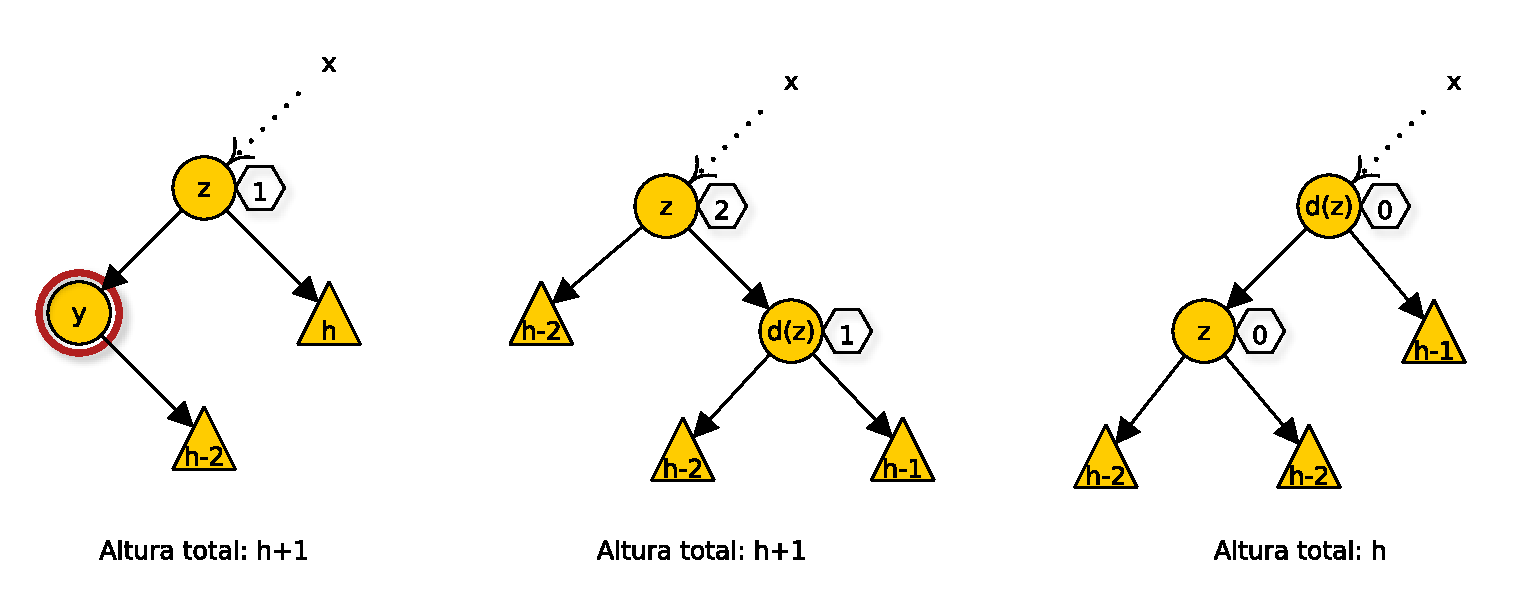
\includegraphics[width=0.70\textwidth]{PeorCasoEliminacionAVL.pdf}
 \caption*{\newline \footnotesize En la primera figura se puede apreciar el nodo $y$ a ser eliminado, junto con su padre $z$ y el FDB de $z$ en el hexagono, la altura total es de $h+1$. En la segunda figura se puede apreciar el estado luego de la eliminaci\'on del nodo $y$ junto con el hijo de derecho de $z$ expandido y los FDB correspondientes a cada nodo recalculados. Finalmente, en la tercera figura se observa el estado luego de la rotaci\'on, lo que genera un decremento en la altura del sub-\'arbol.}
\end{SCfigure}

Para compensar esto ejecutaremos una rotaci\'on hacia la izquierda entre los nodos $z$ y $der(z)$, lo que dejara a $z$ como hijo izquierdo de $der(z)$ y al hijo izquierdo de $der(z)$ como hijo derecho de $z$. Luego de la rotaci\'on los FDB de ambos nodos quedar\'an en $0$ pero la altura del \'arbol se ver\'a reducida en $1$, lo que provocar\'a que el padre original de $z$ (el abuelo de $y$), cambie su FDB de $1$ a $2$. De la misma forma deberemos continuar balanceando el resto de los nodos hasta llegar a la ra\'iz, en donde tendremos que $FDB(izq(raiz)) = 0$, $FDB(der(raiz)) = 1$ y $FDB(raiz) = 2$. Para resolver esta ultima situac\'ion podremos ejecutar una rotaci\'on hacia la derecha entre $izq(raiz)$ y $raiz$, o una rotaci\'on hacia la izquierda entre $der(raiz)$ y $raiz$. Finalmente habremos realizado exactamente $lg(alt(y))$ rotaciones, en donde $alt(y)$ es distancia a la que se encontraba $y$ de la ra\'iz, es decir su altura o nivel. Dentro de este esquema, si seleccionamos a $y$ como uno de los nodos a 
nivel $\
lfloor lg(n) \rfloor$ del \'arbol, entonces tendremos el peor caso de balanceo, por lo que la complejidad de balanceo luego de una eliminaci\'on ser\'a de $O(lg(n))$.

\subsubsection{Complejidades}

\begin{itemize}
 \item \textbf{B\'usqueda} $O(lg(n))$
 \item \textbf{Inserci\'on} $O(lg(n))$
 \item \textbf{Borrado} $O(lg(n))$
 \item \textbf{Espacio} $O(n)$
\end{itemize}

\subsection{B}

Los \'arboles B son \'arboles balanceados de b\'usqueda dise\~nados para trabajar bien en discos r\'igidos u otros dispositivos de almacenamiento secundario. Los \'arboles B son similares a los \'arboles RB, pero son mejores minimizando las operaciones I/O. Varios sistemas de base de datos utilizan \'arboles B o variantes para guardar informaci\'on.

~

Los \'arboles B difieren de los \'arboles RB en el sentido de que los nodos de los \'arboles B pueden tener muchos hijos, desde unos pocos hasta miles. Esto es, que el ''factor de ramificaci\'on`` (breanching factor) de un \'arbol B puede ser bastante grande, sin embargo usualmente depende en las caracter\'isticas de la unidad de disco usada. Este tipo de \'arboles son similares a los \'arboles B en el aspecto de que cada $n-$nodo tiene altura $O(lg(n))$. La altura exacta de un \'arbol B puede ser considerablemente menos que la de un \'arbol RB por su factor de ramificaci\'on, por lo que la base del logaritmo que expresa su altura puede ser mucho mayor.

~

Los \'arboles B generalizan los \'arboles binarios en una forma natural. Si un nodo interno de un \'arbol B $x$ contiene $x.n$ claves, entonces tendr\'a $x.n+1$  hijos. Las claves en un nodo $x$ sirven como puntos de divisi\'on separando los rangos de claves manejados por $x$ en $x.n+1$ sub-rangos, cada uno manejado por un hijo de $x$. Cuando buscamos una clave en un \'arbol B, haremos una decisi\'on entre $x.n+1$ caminos basada en comparaciones con las $x.n$ claves guardadas en el nodo $x$.

~

Un \'arbol B tiene las siguientes propiedades:

\begin{enumerate}
 \item Cada nodo $x$ tiene los siguientes atributos:
 \begin{enumerate}
  \item $x.n$, el numero de claves actualmente guardadas en el nodo $x$.
  \item Las $x.n$ claves, $x.key_1, x.key_2, ..., x.key_{x.n}$, guardadas en orden creciente de forma que $x.key_1\leq x.key_2\leq ...\leq x.key_{x.n}$.
  \item $x.leaf$, un valor booleano que es verdadero si $x$ es una hoja y falso si es un nodo interno.
 \end{enumerate}
 \item Cada nodo interno $x$ adem\'as contiene $x.n+1$ punteros $x.c_1,x.c_2,...,x.c_{x.n+1}$ a sus hijos. Los nodos hojas no tienen hijos, por lo que sus atributos $c_i$ estar\'an indefinidos.
 \item Las claves $x.key_i$ separan los rangos de las claves guardadas en cada sub-\'arbol. Si $k_i$ es cualquier clave guardada en el sub-\'arbol cuya ra\'iz es $x.c_i$, entonces $k_1 \leq x.key_1 \leq k_2 \leq x.key_2 \leq ... \leq x.key_{x.n} \leq k_{x.n+1}$.
 \item Todas las hojas tienen la misma profundidad, la cual ser\'a la altura del \'arbol $h$.
 \item Los nodos tienen cotas inferiores y superiores en el numero de claves que pueden contener. Expresaremos estas cotas en terminos de un entero fijo $t \geq 2$ llamado el grado m\'inimo del \'arbol B:
 \begin{enumerate}
  \item Cada nodo distinto a la ra\'iz debe tener al menos $t-1$ claves. Cada intervalo de nodos distinto que la raiz debe tener al menos $t$ hijos. Si el \'arbol no esta vac\'io, la ra\'iz debe tener al menos una clave.
  \item Cada nodo debe contener como mucho $2t-1$ claves. Entonces, un nodo interno puede tener a lo sumo $2t$ hijos. Diremos que el nodo esta \textbf{lleno} si contiene exactamente $2t - 1$ claves.
 \end{enumerate}
\end{enumerate}

\subsubsection{Arboles 234}
El \'arbol B mas simple ocurre cuando $t=2$. Cada nodo interno puede tener 2, 3 o 4 hijos, por lo que tendremos un \'arbol $2-3-4$. En la practica, valores muchos mas grandes de $t$ nos dar\'an \'arboles B con una altura menor. Gracias a la noci\'on de cotas podremos dar una cota para la altura de un \'arbol B de la forma $h \leq log_t((n+1)/2)$, en donde $n \geq 1$, para cualquier \'arbol B de $n-$claves de altura $h$ y grado minimo $y \geq 2$.

\subsubsection{Inserci\'on en Arboles 234}

Durante la inserci\'on cada vez que encontremos un 3-nodo $x$ empujaremos al nodo del medio hacia su padre $z$ y partiremos el 2-nodo restante en dos 1-nodo. Para nodos distintos de la ra\'iz podremos hacer esto ya que el nodo $z$, por el cual ya habremos pasado, tendr\'a a lo sumo dos claves.  Si es la ra\'iz en la que nos encontramos, crearemos una nueva ra\'iz a la que podamos pasar la clave del medio. Es importante remarcar que los nodos se partir\'an a medida que los descubrimos, si se creo un 3-nodo a partir de la acci\'on de empujar una clave hacia su padre no haremos nada. Las razones por las cuales partimos los 3-nodos son asegurarnos de que haya lugar para la nueva clave en la hoja y para hacer lugar para cualquier clave que sea empujada hacia arriba. La \'unica forma en la que el \'arbol incrementara su profundidad es creando una nueva ra\'iz a causa de una inserci\'on.

\subsubsection{Eliminaci\'on en Arboles 234}

Para la eliminacion, en primer lugar buscaremos la clave a eliminar, si se encuentra en una hoja la eliminaremos y si es un nodo interno una vez encontrada la eliminaremos y buscaremos con la siguiente clave mas alta (que se encontrar\'a en un nodo hoja). Durante la eliminacion se traeran claves desde el padre o los hermanos de forma tal de asegurarnos de al menos tener dos claves en el nodo donde se efectuara la eliminacion (o de donde obtendremos el reemplazo), de cierta forma estaremos haciendo una estrategia inversa a la inserci\'on donde simplemente empujabamos las claves.

~

A medida que busquemos la clave a eliminar o su reemplazo, nos encontraremos en nodos que contengan solo una clave que deberemos lograr que tengan dos. Para lograr esto tendremos distintas estrategias seg\'un los posibles tres casos en donde nos encontremos:

\begin{enumerate}
 \item Intenta robar una clave de los hermanos inmediatamente adyacentes. Si alguno de sus hermanos tiene mas de una clave ejecutara una rotaci\'on para obtenerlo.
 \item Si no hay hermano adyacente al que podamos robarle una clave, robaremos una clave al padre (esto sera posible al menos que sea la raiz) y fusionaremos la misma con el hermano siguiente u anterior (dependiendo de la desigualdad) formando un 3-nodo.
 \item Si no hay hermano adyacente al que podamos robarle una clave, el padre es la ra\'iz y tiene solo una clave, entonces fusionaremos en un 3-nodo los hermanos y la ra\'iz, obteniendo as\'i un nuevo 3-nodo ra\'iz. Este sera el \'unico caso en donde la altura del \'arbol se ver\'a disminuida en una unidad.
\end{enumerate}

Mostraremos los tres casos mediante un ejemplo al cual se le remover\'a la ra\'iz.

\begin{SCfigure}[1][ht!]
 \centering
 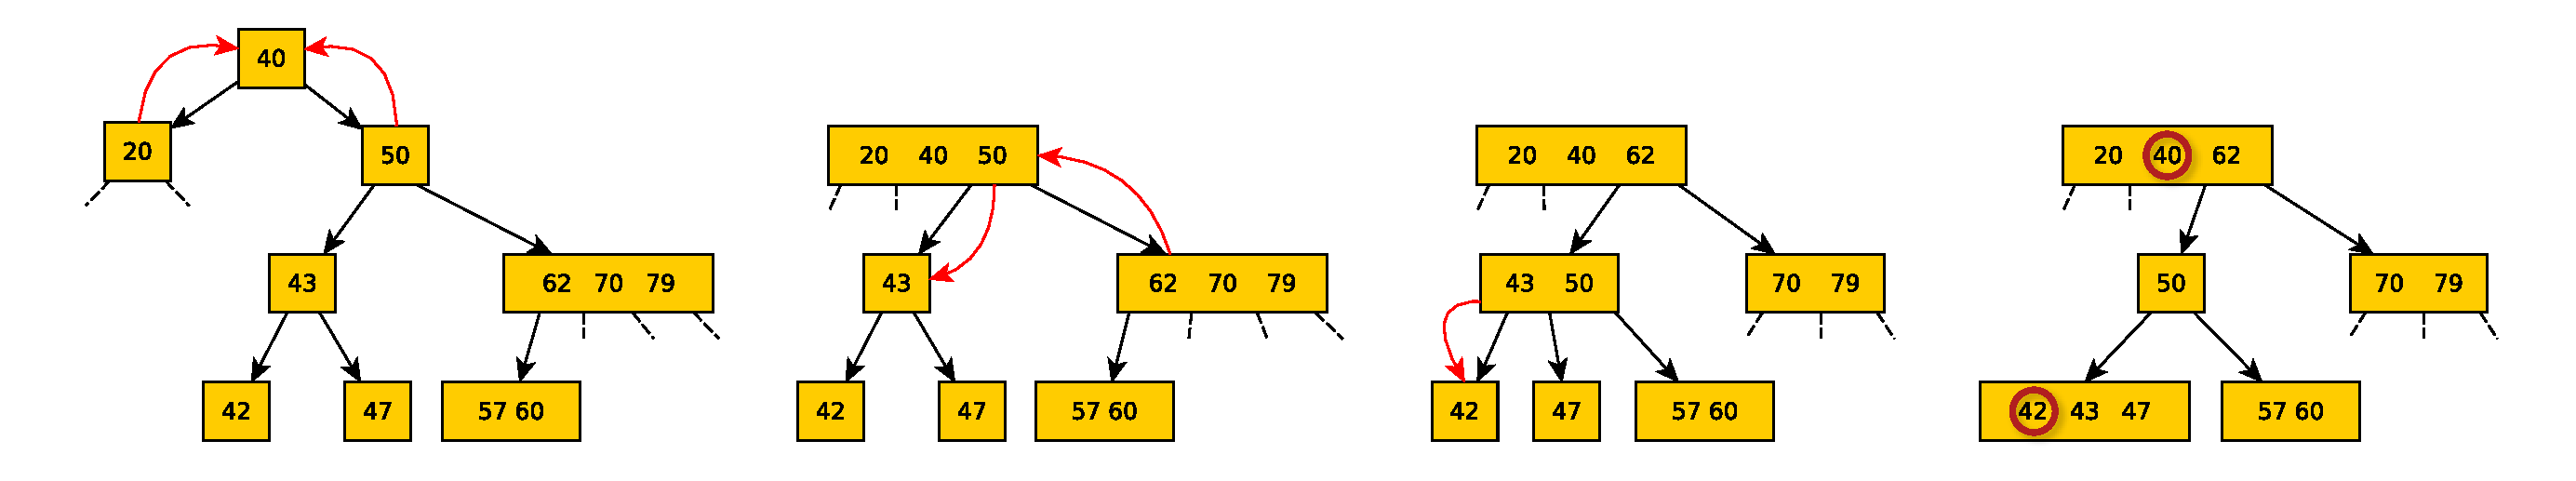
\includegraphics[width=1\textwidth]{EliminacionArboles234.pdf}
\end{SCfigure}

Como queremos remover el $40$, el objetivo sera reemplazarlo por el $42$ que se encuentra en una de las hojas del \'arbol. Una vez parados en el 1-nodo que contiene la clave $50$, veremos que aplica el tercer caso ya que el padre es la ra\'iz, y el \'unico hermano inmediato tiene solo una clave, por lo que haremos una fusi\'on como se aprecia en la segunda figura. Luego descenderemos por la rama dirigida hacia el 1-nodo que contiene el $43$, veremos que en esta instancia el primer caso es el que se ajusta, por lo cual realizaremos una rotaci\'on para terminar con un 2-nodo como se aprecia en la tercera figura. Finalmente en la tercera figura habremos descendido por el nodo que contiene a $42$ pero todav\'ia no podremos usarlo para reemplazar a $40$ ya que es un 1-nodo. En esta situaci\'on el caso que se ajustara ser\'a el segundo, ya que el \'unico hermano inmediato es el $47$, por lo que bajaremos el $43$ y lo fusionaremos con el $47$, llegando as\'i a la cuarta figura en donde podremos eliminar la clave de 
la ra\'iz y 
reemplazarlo por el $42$.

\subsection{Splay trees}

Este tipo de \'arbol tiene su inspiraci\'on en los ABB \'optimos. Los ABB \'optimos son \'arboles cuyos elementos est\'an ubicados mas cerca o lejos de la ra\'iz seg\'un la frecuencia con la que son consultados (similar a la codificaci\'on de Huffman), de esta forma optimizando los tiempos de las operaciones. El problema de este tipo de \'arboles son la rigidez, el desconocimiento de la frecuencia de las operaciones y la variabilidad que pueden sufrir estas ultimas. Los Splay Trees son ABB \'optimos aproximados que se modifican seg\'un la frecuencia de los \'ultimos elementos consultados, de esta forma mantendremos algo cercano a un ABB \'optimo que se ira optimizando para los elementos que consultemos mas frecuentemente.

~

En estos \'arboles, los cuales utilizan exactamente la misma representaci\'on interna que un ABB com\'un sin ning\'un agregado, todas las operaciones toman $O(lg(n))$ en promedio. Cuando nos referimos a en promedio no nos referimos al promedio de los ABB o al Quicksort, no hay aleatorizaci\'on en los Splay Trees. De hecho, una operaci\'on simple puede tomar $\Theta(n)$ en el peor caso en donde $n$ es la cantidad de elementos en el \'arbol. Lo que podemos garantizar entonces es que cualquier secuencia de $k$ operaciones, comenzando con un \'arbol vac\'io, y con el \'arbol no creciendo mas que $>n$ elementos, entonces la secuencia a lo sumo toma $O(k\cdot lg(n))$ en el peor caso. Esto significa que podremos tener algunas pocas operaciones lentas pero la mayor\'ia ser\'an mucho mas r\'apidas, por lo que tendremos un balance en promedio de $lg(n)$ o mejor para cada operaci\'on.

~

Otra ventaja en cuanto a otras estructuras es que los Splay Trees son mucho mas f\'aciles de programar y adem\'as otorgan acceso mas r\'apido a los datos recientemente accedidos, es decir que de cierta forma los Splay Trees tienen ''memoria`` en este aspecto. Esto \'ultimo puede darnos una performance mayor en comparaci\'on a los \'arboles 234 si tenemos un \'arbol grande y solamente accedamos algunos de los elementos ignorando la mayoria de ellos, ya que como estaremos recurriendo frecuentemente a los mismos elementos los accesos en el Splay Tree se dar\'an en $O(1)$.

~

Los Splay Trees, al igual que otros \'arboles balanceados, mantienen su balance mediante rotaciones. El balance de los Splay Trees no es perfecto, es por eso que si bien no nos garantizan una cota de $lg(n)$ en los peores casos los algoritmos utilizados para mantener cierto balance son mucho mas sencillos y r\'apidos que ene estructuras de datos balanceadas mas r\'igidamente. Adem\'as, no nos garantizaran una cota en el peor caso, pero si nos garantizan la cota en la mayor\'ia de las operaciones, lo que en la practica y para la mayor\'ia de los casos los hace igualmente buenos.

~

\subsubsection{B\'usqueda}

Dada una clave $k$, empezaremos a buscar la clave de la misma manera que lo hacemos en un ABB hasta que encontremos la clave $k$ o hasta llegar a un $NIL$ (en el caso de que la clave no sea existente). Sea $x$ el nodo en donde la b\'usqueda termino, contenga o no $k$, elevaremos $x$ a trav\'es de una secuencia de rotaciones, de forma tal que $x$ se vuelva la ra\'iz, llamaremos a esta operaci\'on \textbf{splay}. Las razones por las cuales haremos esto ser\'an, en primer lugar, para mantener los elementos mas consultados en la ra\'iz o cerca de ella, de forma tal de que la consulta de estos sea verdaderamente r\'apida la pr\'oxima vez, y en segundo lugar, como este tipo de \'arboles puede desbalancearse (lo que es usualmente un estado temporal), si nos encontramos en un caso en donde exploremos hasta la profundidad del mismo, las rotaciones evitaran que esto pase de nuevo.

\newpage

Las rotaciones se daran en tres casos:

\begin{enumerate}
 \item \textbf{Zig-zag} $x$ es el hijo izquierdo de un hijo derecho ($LR$) o su caso espejo ($RL$). Siendo $y$ el padre de $x$ y $z$ su abuelo, para resolver este caso haremos una rotaci\'on hacia la izquierda entre $y$ y $x$ y luego una rotaci\'on hacia la derecha entre $x$ y $z$. En el caso espejo realizaremos una rotaci\'on hacia la derecha y luego una hacia la izquierda, dejando a $x$ como la raiz del sub-\'arbol.
 
 \begin{SCfigure}[1][ht!]
 \centering
 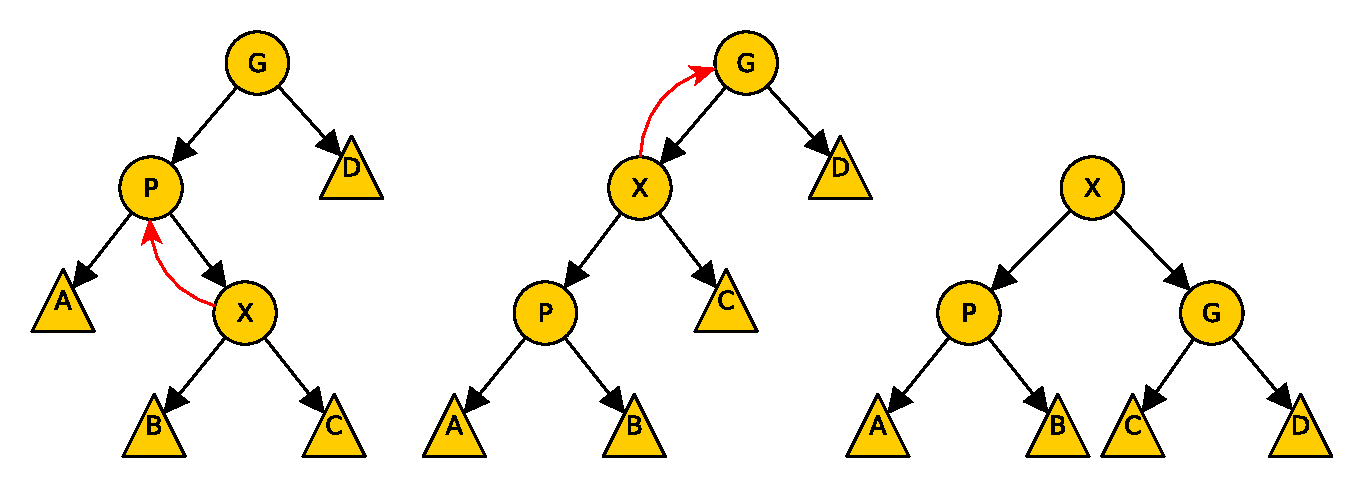
\includegraphics[width=0.5\textwidth]{ZigZagSplay.pdf}
 \end{SCfigure}
 
 \item \textbf{Zig-zig} Este caso tiene una diferencia muy sutil con el caso anterior. Si $x$ es el hijo izquierdo de un hizo izquierdo ($LL$) o su caso espejo ($RR$). Siendo $y$ el padre de $x$ y $z$ su abuelo, para resolver este caso haremos primero una rotaci\'on entre $y$ y $z$ hacia la derecha, y luego ejecutaremos otra rotaci\'on hacia la derecha entre $x$ e $y$, dejando a $x$ como la ra\'iz del sub-\'arbol.
 
 \begin{SCfigure}[1][ht!]
 \centering
 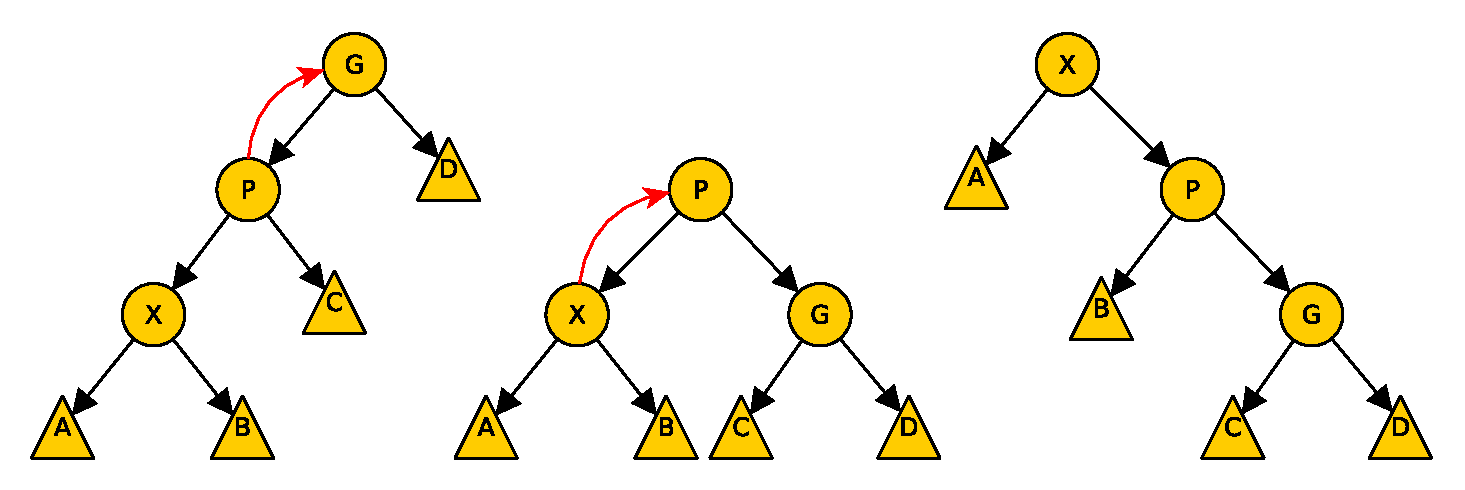
\includegraphics[width=0.5\textwidth]{ZigZigSplay.pdf}
 \end{SCfigure}
 
 ~
 
 \item \textbf{Zig} Este es un caso final que se origina al tener a $x$ a una distancia original impar de la ra\'iz en el momento del acceso. Para solucionar esto, si $x$ es el hijo izquierdo haremos una rotaci\'on hacia la derecha entre $x$ y la ra\'iz, o si $x$ es el hijo derecho haremos una rotaci\'on hacia la izquierda.
\end{enumerate}

Los casos $1$ y $2$ se repetir\'an hasta que $x$ sea la ra\'iz del \'arbol o un hijo de la ra\'iz, lo que dar\'a lugar al caso $3$. En los casos de tengamos un \'arbol totalmente degenerado hacia un lado (de forma tal que sea equivalente a una lista), la b\'usqueda nos costara tiempo $O(n)$ pero las rotaciones Zig-zig lograr\'an acortar la altura del \'arbol a la mitad, de forma tal de que las siguientes operaciones de consulta sean mucho mas eficientes. Esto ultimo se logra gracias a la forma de la rotaci\'on Zig-zig, la cual rota el abuelo y su padre antes que el hijo y su padre, si esto si hiciese en orden inverso obtendr\'iamos un \'arbol totalmente degenerado hacia la direcci\'on opuesta original. 

\subsubsection{Max/Min, Inserci\'on y Eliminaci\'on}

Las dem\'as operaciones del \'arbol usaran la operaci\'on de splay de formas similares ya que es importante para el Splay Tree ejecutar un splay cada vez que realizamos una operaci\'on sobre el mismo, ya que de esta forma el \'arbol se mantiene actualizado y balanceado segun las ultimas operaciones.

\begin{itemize}
 \item En el caso de \textbf{max/min}, una vez encontrado la max/min clave del \'arbol, haremos un splay del nodo que lo contiene.
 \item En el caso de la \textbf{inserci\'on}, una vez insertado el elemento haremos splay sobre el elemento.
 \item En el caso de la \textbf{eliminaci\'on}, una vez eliminado de la misma forma que har\'iamos en un ABB com\'un, sea $x$ el nodo eliminado del \'arbol, ejecutaremos splay sobre el padre de $x$. Si la clave que quer\'iamos eliminar no existe, aun deberemos ejecutar un splay sobre algo, por lo que lo haremos donde termino la b\'usqueda, tal como en la primera operaci\'on.
\end{itemize}

\subsection{Tries}
\subsubsection{Tries compactos}
\subsubsection{Tries Patricia}

\subsection{Red-Black}

Los \'arboles RB son unos de los tantos esquemas en donde son ''balanceados`` para asegurar que las operaciones tomen $O(lg(n))$ en el peor caso. Un \'arbol RB es un \'arbol binario de b\'usqueda con un almacenamiento de un dato extra en cada nodo, su color, el cual puede ser rojo o negro. Restringiendo los colores de los nodos en cualquier camino simple desde la ra\'iz a una hoja, los \'arboles RB se aseguran que no haya camino mas largo que el doble que cualquier otro, de esta forma el \'arbol esta aproximadamente balanceado.

Cada nodo del \'arbol ahora contiene los atributos color, clave, izquierda, derecha y p. Si un hijo o el padre de un nodo no existe, el puntero correspondiente al atributo del nodo contiene el valor $NIL$. Un \'arbol RB tiene las siguientes propiedades:

\begin{enumerate}
 \item Todos los nodos son rojos o negros
 \item La ra\'iz es negra
 \item Cada hoja ($NIL$) es negra
 \item Si un nodo es rojo, entonces ambos hijos son negros.
 \item Por cada nodo, todos los caminos simples desde el nodo a hojas de descendientes tienen el mismo numero de nodos negros.
\end{enumerate}

Como conveniencia para lidiar con las condiciones borde en el c\'odigo del \'arbol RB, usaremos un \'unico centinela para presentar $NIL$. Para un \'arbol RB $T$, el centinela $T.nil$ es un objeto con los mismos atributos que cualquier otro nodo en el \'arbol. Si atributo de color es negro, y sus otros atributos tomaran valores arbitrarios. Usaremos este centinela de forma tal que podamos tratar un hijo $NIL$ de un nodo $x$ como un nodo ordinario cuyo padre es $x$. A pesar de que en cambio podr\'iamos agregar un nodo centinela distinto para cada $NIL$ en el \'arbol, de forma tal que el padre de $NIL$ este bien definido, ese enfoque nos resultara en una perdida de espacio.

Llamaremos al numero de nodos negros de un camino simple desde $x$, pero no incluy\'endolo, hasta una hoja la black-height de un nodo, denominada por $bh(x)$. Por la propiedad $5$, la noci\'on de black-height estar\'a bien definida, dado que todos los caminos simples descendientes desde el nodo tendr\'an la misma cantidad de nodos negros.

\subsubsection{Lema (cota de altura)}
Un \'arbol RB con $n$ nodos internos tiene como mucho altura $2\cdot lg(n+1)$.

~

\textbf{Prueba} Empezaremos mostrando que el sub-\'arbol con su ra\'iz en cualquier nodo $x$ contiene al menos $2^{bh(x)}-1$ nodos internos, esta sera nuestra hip\'otesis inductiva y probaremos la propiedad utilizando inducci\'on en la altura de $x$. 

Para el caso base, si la altura de $x$ es $0$, entonces $x$ debe ser una hoja ($T.nil$), y el sub-\'arbol con su ra\'iz en $x$ efectivamente contiene al menos $2^{bf(h)}-1 = 2^0 -1 = 0$ nodos internos. Para el paso inductivo, consideraremos un nodo $x$ que tiene una altura positiva y es un nodo interno con $2$ hijos (recordar que estamos considerando a los $NIL$ como hijos). Cada hijo tiene una black-height de $bh(x)$ o $bh(x)-1$, dependiendo en si su color es rojo o negro, es decir si suma o no a la black-height. Dado que la altura de un hijo de $x$ es menor que la altura de $x$ en si mismo, podremos aplicar la hip\'otesis inductiva para concluir que cada hijo tiene al menos $2^{bh(x)-1}-1$ nodos internos. Entonces, el sub-\'arbol con su ra\'iz en $x$ contiene al menos $(2^{bh(x)-1}-1) + (2^{bh(x)-1}-1) + 1 = 2^{bh(x)}-1$ nodos internos, lo que prueba la propiedad.

~

Para concluir la prueba del lema, sea $h$ la altura del \'arbol y de acuerdo con la propiedad $4$, al menos la mitad de los nodos en un camino simple desde la ra\'iz a una hoja, sin incluir la ra\'iz, deben ser negros (ya que no hay restricci\'on sobre un nodo negro con un hijo negro, y para tener la m\'inima cantidad de negros deber\'an estar alternados con rojos). En consecuencia, la black-height de la ra\'iz debe ser al menos $h/2$, entonces $n \geq 2^{h/2}-1 \implies n+1 \geq 2^{h/2}$. Si aplicamos logaritmo a ambos lados nos queda que $lg(n+1) \geq h/2 \implies h \leq 2 \cdot lg(n+1)$, lo que prueba el lema.

\subsubsection{B\'usqueda, m\'aximo y m\'inimo}

Como consecuencia directa del lema las operaci\'on de b\'usqueda, y por lo consecuente las de m\'aximo y m\'inimo, tendr\'an tiempo $O(lg(n))$ en el peor caso, en un \'arbol RB.

\subsubsection{Inserci\'on}

Podremos insertar un nodo nuevo en un \'arbol RB de $n$ nodos en tiempo $O(lg(n))$. Para lograrlo, haremos algo muy parecido a la inserci\'on del \'arbol binario de b\'usqueda. Insertaremos el nuevo nodo $z$ tal como lo har\'iamos en un \'arbol binario de b\'usqueda normal, y luego le dar\'iamos color rojo. Para garantizar que las propiedades del \'arbol RB se mantengan, realizaremos un procedimiento de reacomodaci\'on que recolorear\'a y ejecutara rotaciones sobre los nodos existentes.

~

En la inserci\'on de $z$ se mantendr\'an las propiedades $1$ y $3$, ya que no estaremos introduciendo un nuevo color y ya que $z$ tendr\'a dos hijos $NIL$ que estar\'an pintados de negro. Por lo que, las \'unicas propiedades que pueden llegar a violar ser\'an la propiedad $2$, que requiere que la ra\'iz sea negra, y la propiedad $4$, que dice que un nodo rojo no puede tener un hijo rojo. Ambas posibles violaciones son a causa de que $z$ sea pintado rojo.

~

Deberemos considerar seis casos para la reacomodaci\'on, la cual se realizara en un ciclo hasta que el \'arbol sea correcto, pero tres de los seis casos son sim\'etricos a los otros tres, por lo que realmente solamente necesitaremos considerar tres casos. Distinguiremos el caso $1$ del caso $2$ y $3$ observando el color del hermano del padre de $z$, dicho de otra forma, el t\'io de $z$. Es aqu\'i donde los $6$ casos pasan a ser $3$. Si $z.p$ es el hijo derecho, entonces el t\'io sera $z.p.p.izq$, de lo contrario sera $z.p.p.der$. Para trabajar sobre los $3$ casos distintos, haremos de cuenta que $z.p$ es el hijo izquierdo, despu\'es de todo si es el derecho solamente habr\'a que hacer un cambio de palabras. Si el color del t\'io $y$ es rojo, entonces ejecutaremos el caso $1$, de otra forma el control pasa al caso $2$ y $3$. En los $3$ casos, el abuelo $z.p.p$ es negro, dado que el padre $z.p$ es rojo, y la propiedad $4$ es solo violada entre $z$ y $z.p$.

\begin{itemize}
 \item \textbf{Caso 1: El t\'io $y$ de $z$ es rojo} Como $z.p.p$ es negro, podremos pintar $z.p$ y $y$ negros, solucionando el problema entre $z$ y $z.p$, y podremos pintar $z.p.p$ de negro par mantener la propiedad $5$. Deberemos repetir la reacomodaci\'on definiendo a $z = z.p.p$. El puntero de $z$ se mueve dos niveles mas arriba en el \'arbol.
 \item \textbf{Caso 2: El t\'io $y$ de $z$ es negro y $z$ es un hijo derecho} En este caso utilizaremos una rotaci\'on hacia la izquierda para transformar la situaci\'on en el caso $3$, en donde $z$ sera el hijo izquierdo. Dado que $z$ y $z.p$ son rojos, la rotaci\'on no afecta el black-height de los nodos o la propiedad $5$. $z$ ahora sera $z.p$.
 \item \textbf{Caso 3: El t\'io $y$ de $z$ es negro y $z$ es un hijo izquierdo} Si entramos en el caso $3$ directamente o a trav\'es del caso $2$, el t\'io $y$ de $z$ es negro, ya que de otra forma hubi\'esemos ejecutado el caso $1$. En este caso ejecutaremos una rotaci\'on hacia la derecha entre el padre $z.p$ y su abuelo $z.p.p$, lo que dejar\'a al abuelo de $z$ como hermano de $z$. Haciendo un intercambio de colores entre el padre de $z$ y el ahora hermano de $z$, lograremos restablecer la propiedad $4$ y adem\'as nos aseguramos de mantener la propiedad $5$.
 \end{itemize}

\begin{SCfigure}[1][ht!]
 \centering
 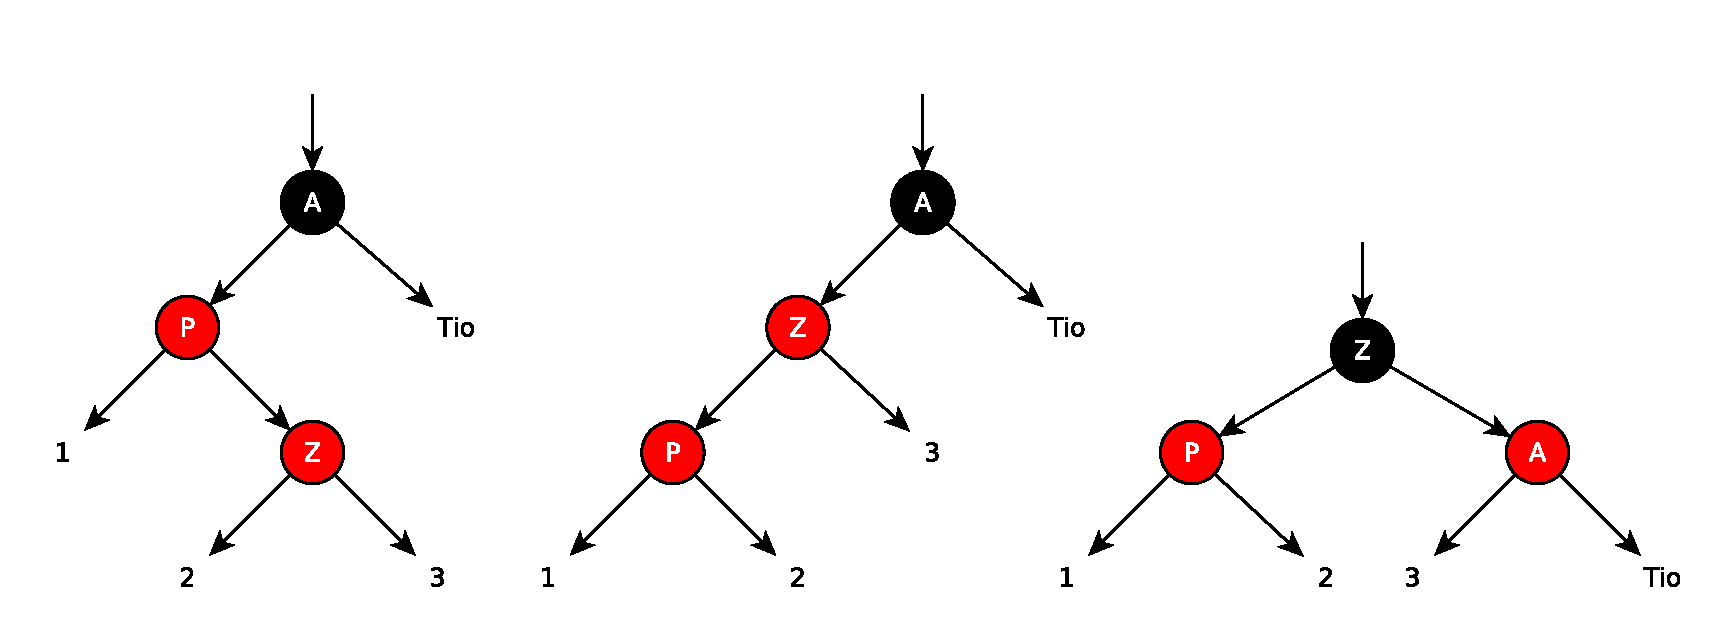
\includegraphics[width=0.75\textwidth]{RBCaso3.pdf}
 \caption*{\newline \footnotesize $z$, $p$ y $a$ representan el nodo nuevo $z$, su padre y su abuelo, respectivamente. En el primer momento estaremos en el caso $2$ y una vez ejecutada la rotaci\'on pasaremos al segundo momento. Si bien no cambiaremos los nombres por claridad, el puntero $z$ ahora estar\'a apuntando a $p$. En este momento estar\'iamos en el caso $3$, haciendo una rotaci\'on hacia la derecha mas pasar\'iamos al ultimo estado que cumplir\'a todas las propiedades.}
\end{SCfigure}
 
Dado que la altura de un \'arbol RB de $n$ nodos pertenece a $O(lg(n))$, la inserci\'on principal del nuevo nodo $z$ tomar\'a tiempo $O(lg(n))$. Cuando ejecutamos la reacomodaci\'on, solo es necesario ejecutarla nuevamente cuando ocurre el primer caso, y cuando sucede el puntero de $z$ se mueve dos niveles hacia arriba del \'arbol. Por lo tanto el numero de veces m\'aximo que deberemos ejecutar la reacomodaci\'on sera $O(lg(n))$, por lo que la inserci\'on tomar\'a en total $O(lg(n))$.

\subsubsection{Eliminaci\'on}

Eliminar un nodo de un \'arbol RB puede ser un poco mas complicado que insertar un nodo. El procedimiento para eliminar un nodo de un \'arbol RB esta basado en la eliminaci\'on del \'arbol binario de b\'usqueda.

%TODO: Falta completar esto, pagina 323 del cormen.

\subsubsection{Complejidades}

\begin{itemize}
 \item \textbf{B\'usqueda} $O(lg(n))$
 \item \textbf{Inserci\'on} $O(lg(n))$
 \item \textbf{Borrado} $O(lg(n))$
 \item \textbf{Espacio} $O(n)$
\end{itemize}

\newpage
\section{Hash}

Muchas aplicaciones requieren un conjunto din\'amico que solo soporte las operaciones de diccionario inserci\'on, b\'usqueda y eliminaci\'on. Una tabla de hash es una estructura de datos efectiva para implementar diccionarios. Si bien buscar un elemento en una tabla de hash puede tardar tanto como buscar un elemento en una lista enlazada ($\Theta(n)$ en el peor caso), en la practica la tabla de hash tiene una muy buena performance. Bajo asunciones razonables, el tiempo promedio de buscar un elemento en una tabla de hash es de $O(1)$.

\subsection{Direccionamiento abierto}
\subsection{Barrido lineal}
\subsection{Barrido cuadr\'atico}
\subsection{Hashing doble}
\subsection{Hashing din\'amico o extensible}

\chapter{Algoritmos}

\section{Eliminaci\'on de la recursion}

La motivaci\'on de la eliminaci\'on de la recursion es b\'asicamente optimizar funciones recursivas mediante distintas formas. Para hacerlo se intentara cumplir ciertos objetivos como no repetir los c\'alculos (generalmente en problemas que presenten sub-estructura \'optima), no recorrer una estructura mas de una vez (o intentar hacerlo la menor cantidad posible de veces) y finalmente eliminar la recursion, ya que si bien una funci\'on iterativa y una recursiva podr\'an tener complejidades asint\'oticamente iguales, en la practica las funciones iterativas son mas o\'ptimas por diferencias de constantes (b\'asicamente por no tener llamadas recursivas).

~

\textbf{Inmersi\'on de rango} Agregar un nuevo par\'ametro de salida a la funci\'on, es decir si la salida original era un entero, ahora sera una dupla de enteros. La idea del nuevo par\'ametro que agregamos es darnos ''algo mas`` que lo estrictamente necesario de forma tal que nos sirva para calcular mas eficientemente otro resultado y as\'i reducir la complejidad. Esta t\'ecnica tambi\'en es conocida como \textbf{generalizaci\'on de funciones}.

~

\textbf{Inmersi\'on de dominio} En este caso agregaremos un par\'ametro de entrada que va conteniendo resultados intermedios. De esta forma podremos optimizar la complejidad de problemas que presenten subestructura \'optima.

~

\textbf{Inmersion de genero} Se amplia el dominio de alg\'un par\'ametro de la funci\'on. Por ejemplo de naturales a enteros.

~

\textbf{Recursion a cola} Esta sera una clase de funciones recursivas lineales en donde su ultimo paso es la llamada recursiva y adem\'as es \'unica. La propiedad de estas es que pueden ser transformadas autom\'aticamente a funciones iterativas.

~

\textbf{Recursivas lineales no a cola} Son aquellas que tienen una \'unica llamada recursiva (por eso lineales) pero esta no es la ultima operaci\'on. Una funci\'on de este tipo puede ser aquella que tenga un condicional para separar entre el caso base y el caso recursivo. Este tipo de funciones pueden tambi\'en ser convertidas autom\'aticamente.

~

\textbf{Recursivas no lineales} Ser\'an aquellas que tienen mas de una llamada recursiva. Pueden ser \textbf{m\'ultiples} en donde contienen varias llamadas pero no es la ultima operaci\'on o \textbf{anidadas}, las cuales tienen mas de una llamada recursiva pero anidadas y adem\'as la llamada es la ultima operaci\'on.

~

\textbf{Folding/Unfolding} Es desplegado consiste en reemplazar la definici\'on de la funci\'on por su expresi\'on. El plegado puede pensarse como la inversa de la anterior. Se trata de reemplazar la definici\'on de una expresi\'on por una llamada a funci\'on.

\newpage
\section{Dividir y Conquistar}

La metodolog\'ia consiste en \textbf{dividir} el problema en un numero de subproblemas que son instancias mas chicas del mismo problema, \textbf{conquistar} los subproblemas resolvi\'endolos recursivamente y cuando sean suficientemente chicos resolverlos de una forma directa y \textbf{combinar} las soluciones de los subproblemas en la soluci\'on para el problema original.

Cuando los subproblemas son suficientemente grandes para resolverlos recursivamente, llamaremos al \textbf{caso recursivo}. Una vez que los subproblemas se vuelvan suficientemente chicos, diremos que la recursion ''toco fondo`` y que habremos llegado al \textbf{caso base}. A veces, en adici\'on a los subproblemas que son instancias mas chicas del mismo problema, deberemos resolver problemas que no son exactamente lo mismo que el problema original. Consideraremos resolver dichos subproblemas como una parte del paso de combinaci\'on.

\subsection{Recurrencias}

Las recurrencias van a la par con el paradigma de DyC, ya que nos dan una forma natural de caracterizar los tiempos de los algoritmos que hagan uso del paradigma. Una recurrencia es una ecuaci\'on o inecuaci\'on que describe una funci\'on en t\'erminos de su valor en entradas mas chicas. Las recurrencias pueden tomar muchas formas. Por ejemplo, un algoritmo recursivo podr\'a dividir los subproblemas en tama\~nos desiguales, tales como $2/3$ a $1/3$. Si los pasos de dividir y combinar toman tiempo lineal, tal algoritmo nos dar\'a la recurrencia $T(n) = T(2n/3) + T(n/3) + \Theta(n)$. Los subproblemas no estas necesariamente acotados a ser una fracci\'on constante del tama\~no del problema original. Por ejemplo, si en cada paso disminuy\'eramos 1 solo elemento, nos quedar\'ia una recurrencia del tipo $T(n) = T(n-1) + \Theta(1)$. Habr\'a 3 m\'etodos para resolver recurrencias, esto es para obtener las cotas asint\'oticas ``$\Theta$ o ''$O$`` de la soluci\'on:

\begin{itemize}
 \item En el m\'etodo de substituci\'on, conjeturaremos una cota y luego la probaremos utilizando inducci\'on matem\'atica.
 \item En el m\'etodo del \'arbol de recursion, convertiremos la recurrencia en un \'arbol cuyos nodos representaran los costos de varios niveles de la recursion. Usaremos t\'ecnicas para acotar sumatorias para resolver la recurrencia.
 \item El m\'etodo maestro proveer\'a cotas para recurrencias de la forma $T(n) = aT(n/b) + f(n)$, en donde $a \geq 1$, $b > 1$ y $f(n)$ es una funci\'on dada, las recurrencias de este tipo se presentan muy frecuentemente. Para utilizar el m\'etodo maestro ser\'a necesario memorizar tres casos, pero una vez hecho, podremos determinar cotas asint\'oticas muy f\'acilmente para recurrencias simples.
\end{itemize}

~

Ocasionalmente podremos ver recurrencias que no son igualdades sino que ser\'an desigualdades, como lo es $T(n) \leq 2T(n/2) + \Theta(n)$. Dada que dicha recurrencia solo nos da noci\'on de una cota superior en $T(n)$, daremos la soluci\'on con notaci\'on $O$ en vez de $\Theta$. De igual forma, con la desigualdad invertida $T(n) \geq 2T(n/2) + \Theta(n)$, la recurrencia solo nos dar\'a la idea de una cota inferior de $T(n)$, por lo tanto usaremos $\Omega$ para dar su soluci\'on.

\subsubsection{M\'etodo de substituci\'on}

El m\'etodo de substituci\'on para resolver recurrencias se compone de dos pasos. El primero de ellos es conjeturar una formula general de la soluci\'on y el segundo es usar inducci\'on matem\'atica para encontrar las constantes y mostrar que la soluci\'on funciona. Veamos este m\'etodo mediante un ejemplo. Tomemos la recurrencia perteneciente a Merge Sort.

\begin{equation*}
  T(n) = \begin{cases}
	      1         		& \text{si} \ n = 1 \\
	      2T(n/2) + n         	& \text{caso contrario}
	  \end{cases}
\end{equation*}

~

El caso base hace referencia a cuando nuestro arreglo tiene tama\~no $1$, en cuyo caso devolveremos el arreglo sin ejecutar ninguna operaci\'on sobre el, y el caso recursivo hace referencia a la recursion del arreglo sobre cada una de sus mitades (siendo as\'i divide) y luego uni\'endolo en tiempo $n$ (siendo el conquer). En primer lugar vamos a acotar a $n$ por el m\'ultiplo de $2$ mayor o igual mas cercano, quedando as\'i $n \leq 2^k$ para alg\'un $k \in N$. Luego, reescribiremos a $T(n)$ haciendo el reemplazo por $k$.

\begin{equation*}
  T(2^k) = \begin{cases}
	      1         		& \text{si} \ k = 0 \\
	      2T(2^{k-1}) + 2^k        	& \text{caso contrario}
	  \end{cases}
\end{equation*}

~

Probemos alguno de sus valores y analicemos los resultados correspondientes para encontrar alg\'un patr\'on que nos ayude a visualizar la formula general.

\begin{equation*}
\begin{align*}
 T(2^0) & = 1 \\
 T(2^1) & = 2 \cdot T(2^0) + 2^1 = 2 + 2 & = 2^1 + 1 \cdot 2^1 \\
 T(2^2) & = 2 \cdot T(2^1) + 2^2 & = 2^2 + 2 \cdot 2^2 \\
 T(2^3) & = 2 \cdot T(2^2) + 2^3 &= 2^3 + 3 \cdot 2^3 \\
 T(2^4) & = 2 \cdot T(2^3) + 2^4 &= 2^4 + 4 \cdot 2^4 \\ \\
 T(2^k) & = 2^k + k \cdot 2^k
\end{align*}
\end{equation*}

~

Probaremos que esta conjetura es valida utilizando inducci\'on en $N$. El caso base es trivial, ya que $T(2^0) = 2^0 + 0 \cdot 2^0 = 0$, por lo que coincide con la definici\'on. Luego para el paso inductivo, consideraremos que la formula vale hasta $k$ (nuestra hip\'otesis inductiva) y queremos ver que vale para $k+1$ (nuestra tesis inductiva).

\begin{equation*}
 T(2^{k+1}) = 2T(2^k) + 2^{k+1} \overset{HI}{=} 2(2^k + k \cdot 2^k) + 2^{k+1} = 2^{k+1} + k \cdot 2^{k+1} + 2^{k+1} = 2^{k+1} + (k+1) \cdot 2^{k+1}
\end{equation*}

Por lo que nuestra tesis inductiva inductiva sera v\'alida y la formula general que encontramos valdr\'a para todo $n \in N$. Como $n \leq 2^k \iff log(n) \leq k$ para alg\'un $k$, tendremos que $T(n) \leq n + n \cdot log(n)$ y por lo tanto $T(n) \subseteq O(n \cdot log(n))$. De la misma forma, si utilizamos el m\'ultiplo de $2$ menor o igual mas cercano a $n$, obtendremos la misma cota pero perteneciente a $\Omega(n \cdot log(n))$, por lo que nos implicara que $T(n) \subseteq \Theta(n \cdot log(n))$. 

~

La ultima formula puede ser generalizada cambiando sus constantes por variables.

\begin{equation*}
  T(2^k) = \begin{cases}
	      c         		& \text{si} \ k = 0 \\
	      2T(2^{k-1}) + f(2^k)        	& \text{caso contrario}
	  \end{cases}
\end{equation*}

~

Luego, la conjetura quedar\'ia de la forma $T(2^k) = 2^k \cdot c + \sum_{i=1}^k 2^{k-i} f(2^i) \leq 2^k \cdot c + k \cdot 2^k f(2^k)$. Si definimos a $f(n) = n$ y a $c=1$, podremos observar que nos quedar\'a $T(2^k) \leq 2^k + k \cdot 2^{k+1}$ la cual solo difiere en una constante ya que utilizamos una cota mas bruta, pero pertenecer\'a a la misma clase que la funci\'on anterior.

\subsubsection{M\'etodo del \'arbol de recursion}

Si bien podremos usar el m\'etodo de substituci\'on para proveer una prueba suficiente de que una soluci\'on a una recurrencia es correcta, tendremos problemas en encontrar una buena conjetura, algo en lo que nos ayudara el \'arbol de recursion. 

En un \'arbol de recursion, cada nodo representa el costo de un de un solo subproblema en alg\'un momento del conjunto de invocaciones recursivas, el nodo principal representar\'a el costo inmediato inicial de la funci\'on (sin contabilizar la recursion) y los nodos adyacentes a el, es decir el primer nivel, representar\'an el costo inmediato de cada paso. Como hojas del \'arbol tendremos los casos base de la recursion. Para obtener nuestra conjetura, sumaremos los costos de cada uno de los niveles del \'arbol para obtener un conjunto de costos por nivel, y luego sumaremos todos los conjuntos por nivel para obtener el costo total de todos los niveles de la recursion.

~

Un \'arbol de recursion es el mejor m\'etodo para generar una buena conjetura, que luego podremos verificar utilizando el m\'etodo de substituci\'on. Cuando utilizamos el m\'etodo del \'arbol del recursion para generar una conjetura buena, por lo general es tolerable un leve grado de ''descuido``, dado que luego estaremos verificando la conjetura. Si somos suficientemente cuidadosos al dibujar el \'arbol de recursion y sumar los costos, podremos usar el \'arbol de recursion como una prueba directa para la soluci\'on de una recurrencia.

\subsubsection{M\'etodo maestro}

El m\'etodo maestro provee una receta para resolver recurrencias que tengan la forma:

\begin{equation*}
  T(n) = \begin{cases}
	      \Theta(1)         		& n=1 \\
	      a \cdot T(n/b) + f(n)        	& n > 1
	  \end{cases}
\end{equation*}

En donde $a \geq 1$ y $b>1$ son constantes y $f(n)$ es una funci\'on asint\'oticamente positiva. Para usar el m\'etodo maestro, habr\'a que memorizar tres casos, pero una vez hecho se podr\'an resolver recurrencias muy f\'acilmente, muchas veces sin la necesidad de usar l\'apiz y papel. 

~

El m\'etodo maestro tiene su base en el teorema maestro, el cual dice que siendo $a\geq 1$ y $b>1$ constantes, $f(n)$ una funci\'on y $T(n)$ esta definido en los enteros no-negativos por la recurrencia anterior, entonces $T(n)$ tiene las siguientes cotas asint\'oticas:

\begin{itemize}
 \item Si $f(n) \subseteq O(n^{log_b(a)-\epsilon})$ para alguna constante $\epsilon > 0$, entonces $T(n) \subseteq \Theta(n^{log_b(a)})$.
 \item Si $f(n) \subseteq \Theta(n^{log_b(a)})$, entonces $T(n) \subseteq \Theta(n^{log_b(a)} \cdot lg(n))$.
 \item Si $f(n) \subseteq \Omega(n^{log_b(a)+\epsilon})$ para alguna constante $\epsilon > 0$, y si existe alguna constante $c < 1$ y se cumple que $af(n/b) \leq cf(n)$ a partir de un $n$ suficientemente grande, entones $T(n) \subseteq \Theta(f(n))$.
\end{itemize}

En cada uno de los tres casos, comparamos la funci\'on $f(n)$ con la funci\'on $n^{log_b(a)}$. Intuitivamente, la polinomialmente m\'as grande de las dos funciones determina la soluci\'on a la recurrencia. En el primer caso, la funci\'on $n^{log_b(a)}$ es polinomialmente m\'as grande, entonces la soluci\'on ser\'a $\Theta(n^{log_b(a)})$. En el tercer caso si $f(n)$ significa que es la funci\'on polinomialmente m\'as grande, entonces la soluci\'on ser\'a $T(n) \subseteq \Theta(f(n))$, la condici\'on de regularidad en este caso esta presente para asegurarse de que $f(n)$ sea polinomialmente mas grande. Finalmente, en el segundo caso, las dos funciones son ''del mismo tama\~no``, esto quiere decir que cualquiera puede ser utilizada como cota asint\'otica de la otra, se multiplicar\'an por un factor logar\'itmico y la soluci\'on ser\'a $T(n) \subseteq \Theta(n^{log_b(a)} \cdot lg(n)) \subseteq \Theta(f(n) \cdot lg(n))$. Es importante remarcar que el teorema maestro no cubre todos los casos de $f(n)$, por lo cual 
habr\'a algunos casos que caer\'an en las brechas entre alguno de los casos, puntualmente cuando $f(n)$ sea mas grande o mas chica que $n^{log_b(a)}$ asint\'oticamente pero no lo sea polinomialmente.

~

Para utilizar el teorema maestro simplemente debemos determinar a que caso pertenece la recurrencia (si es que lo hace) y escribir la respuesta. Algunos ejemplos de uso del teorema maestro son:

\begin{itemize}
 \item En la recurrencia $T(n) = 9T(n/3) + n$ tendremos que $a=9$, $b=3$ y $f(n)=n$, por lo que tendremos que $n^{log_b(a)} = n^{log_3(9)} = n^2 \subseteq \Theta(n^2)$. Como $f(n) \subseteq O(n^{2-\epsilon})$ con $\epsilon = 1$, entonces podremos aplicar el primer caso del teorema maestro por lo que la soluci\'on a esta recurrencia ser\'a $T(n) \subseteq \Theta(n^2)$.
 
 \item En la recurrencia $T(n) = T(2n/3) + 1$ tendremos que $a=1$, $b=3/2$ y $f(n) = 1$, por lo que tendremos que $n^{log_b(a)} = n^{log_{3/2}(1)} = n^0 \subseteq \Theta(1)$. Como $f(n) \subseteq O(1)$ con $\epsilon = 0$, como $\epsilon > 0$ para que pueda pertenecer al primer caso, la soluci\'on a esta recurrencia se ajusta al segundo caso del teorema maestro, por lo que $T(n) \subseteq \Theta(n^2)$.
 
 \item En la recurrencia $T(n) = 3T(n/4) + n \cdot lg(n)$ tendremos que $a=3$, $b=4$ y $f(n) = n \cdot lg(n)$, por lo que tendremos que $n^{log_b(a)} = n^{log_4(3)} = 0.79$. Con $epsilon \approx 0.2$ tendremos que $f(n) \subseteq \Omega(n)$, lo que se acerca al tercer caso del teorema maestro si podemos cumplir la condici\'on de regularidad. Sea $af(n/b) \leq cf(n) \implies 3f(n/4) \leq cf(n) \implies 3nlg(n/4)/4 \leq cnlg(n)$ lo cual se cumplir\'a para todo $c \geq 3/4$ y para un $n$ suficientemente grande. Esto nos dice que la soluci\'on de la recurrencia es entonces $T(n) \subseteq \Theta(lg(n))$.
 
 \item En la recurrencia $T(n) = 2T(n/2) + n \cdot lg(n)$ tendremos que $a=2$, $b=2$ y $f(n) = n \cdot lg(n)$, por lo que tendremos que $n^{log_b(a)} = n^{log_2(2)} = n$. El tercer caso del teorema maestro parece ajustarse ya que $f(n) \subseteq \Omega(n)$ con $\epsilon = 0$. El problema es que $\epsilon$ debe ser mayor a $1$, y en el segundo caso del teorema la cota superior esta por debajo de $f(n)$. El problema en este caso es que $f(n)$ es asint\'oticamente mas grande que $n$ pero no lo es polinomialmente, por lo que la recurrencia cae en la brecha entre el segundo y tercer caso. En este caso el teorema maestro no decide nada respecto a la recurrencia.
 
 \item En la recurrencia $T(n) = 2T(n/2) + n$, que corresponde al merge sort, tendremos que $a=2$, $b=2$ y $f(n) = n$, por lo que tendremos que $n^{log_b(a)} = n^{log_2(2)} = n$. Luego, esto cae en el segundo caso del teorema ya que $f(n) \subseteq \Theta(n)$, por lo que $T(n) \subseteq \Theta(nlg(n))$.
\end{itemize}

\subsection{En resumen}

La metodolog\'ia consiste en dividir un problema en problemas similares pero mas chicos, en resolver estos problemas menores hasta que podamos resolverlos de forma ADHOC y luego combinar las soluciones de los problemas menores para obtener la soluci\'on del problema original. Este m\'etodo tiene sentido siempre y cuando la divisi\'on y la combinaci\'on no sean excesivamente caras.

~

El esquema general de dividir y conquistar consiste en:

\begin{itemize}
 \item Si $X$ es suficientemente chico, entonces resolveremos el problema de forma ADHOC.
 \item En caso contrario, haremos una descomposici\'on en sub-instancias $X_1, X_2, ..., X_k$, en donde para cada una tendremos $Y_i \gets DC(X_i)$ sub-soluciones, que luego combinaremos las $Y_i$ soluciones para construir la soluci\'on general para $X$.
\end{itemize}

\newpage

\section{Ordenamiento}

\subsection{Cota inferior para algoritmos basados en comparaciones}

Una lista de $n$ elementos distintos puede tener $n!$ permutaciones o formas de orden distintas. Luego, una cota arbitrariamente mayor para $n! \leq n \cdot n \cdot ... \cdot n = n^n$ y una cota arbitrariamente menor podra ser $n! \geq n/2 \cdot n/2 \cdot ... \cdot n/2 = n/2^{n/2}$. Luego, ambas cotas perteneceran a $\Theta(n log(n))$ si les aplicamos un logaritmo, lo que nos implicara que $log(n!) \in \Theta(n lg(n))$.
Todas las decisiones estaran basadas en comparar claves, tipicamente mediante ifs, es decir que estan basadas en resultados booleanos. Un algoritmo de ordenamiento correcto debe generar una secuencia distinta de comparaciones booleanas para cada permutacion distinta de $1.. n$. Como habra $n!$ diferentes permutaciones en una secuencia de $n$ elementos, deberemos tener $n!$ secuencias distintas de comparaciones. Si un algoritmo hace $\leq d$ preguntas booleanas, generara $\leq 2^d$ secuencias distintas de respuestas booleanas, y por lo tanto:

\begin{equation*}
 n! \leq 2^d \implies lg_2(n!) \leq d \implies d \in \Omega(n \cdot lg(n))
\end{equation*}

~

No podremos preguntar $d$ preguntas en menos de $d$ tiempo, si suponemos un tiempo acotado para cada preguntar, por lo que el algoritmo gasta $\Theta(d)$ tiempo preguntando $d$ preguntas. Por lo que todo algoritmo de ordenamiento basado en comparaciones toma en el peor caso $\Omega(n \cdot lg(n))$ tiempo. Algoritmos mas r\'apidos que estos deber\'an hacer decisiones de $q$-caminos para un $q$ grande.

\subsection{Insertion sort}

Es un algoritmo de ordenamiento in-place (es decir que no consume demasiada memoria adicional para ordenar la lista) y corre en tiempo $n^2$ en el peor caso. El invariante de este algoritmo es que la lista $S$ este ordenada. El algoritmo funcionara teniendo una lista $S$ que comenzara vacia y una lista sin ordenar $I$ de $n$ elementos, en cada paso obtendremos un elemento de $n$ y lo \textbf{insertaremos} ordenadamente en $S$, $S$ e $I$ pueden ser sub-arreglos del arreglo original. En el caso que tengamos $n$ claves fuera de lugar, el tiempo es de $O(w)$ en donde $w$ es el numero de ''intercambios`` a realizar. Si utilizamos un \'arbol balanceado de b\'usqueda como la estructura en $S$ el algoritmo se volver\'a $O(n\cdot lg(n))$ aunque sera mas lento que otros algoritmos de b\'usqueda por las constantes ocultas del \'arbol balanceado.

\subsection{Selection sort y Heap sort} 

Es un algoritmo de ordenamiento in-place (es decir que no consume demasiada memoria adicional para ordenar la lista) y corre en tiempo $n^2$ en el peor caso. El invariante de este algoritmo es que la lista $S$ este ordenada. El algoritmo funcionara teniendo una lista $S$ que comenzara vacia y una lista sin ordenar $I$ de $n$ elementos, en cada paso \textbf{seleccionaremos} el m\'inimo elemento de $I$ y lo insertaremos al final en $S$, $S$ e $I$ pueden ser sub-arreglos del arreglo original.

Si cambiamos $I$ por un min-heap, podremos realizar la operaci\'on de encontrar un elemento m\'inimo en tiempo $O(lg(n))$, dejando al algoritmo con tiempo total en $O(n\cdot lg(n) + n) \subseteq P(n\cdot lg(n))$, en donde la suma en el primer caso ser\'a causada por convertir el arreglo en un heap. Esta ultima modificaci\'on nos dar\'a el algoritmo denominado como Heap sort, el cual tambi\'en ser\'a un ordenamiento in-place ya que el \'arbol del heap podr\'a ser guardado en un arreglo. Una optimizaci\'on importante para evitar algunas constantes a la hora de implementar el Heap sort es representar el mismo a la inversa de lo que normalmente lo har\'iamos en el arreglo, dejando la ra\'iz del \'arbol en el final del mismo. Esto provocara que a medida que saquemos el m\'inimo elemento del arreglo, el mismo vaya a parar (por el comportamiento mismo de la eliminaci\'on del heap) al comienzo del arreglo, que por definici\'on del tama\~no del heap, estar\'a fuera del mismo. Si queremos implementar esto mismo 
utilizando la representaci\'on cl\'asica del Heap sort, deberemos invertir el orden del arreglo una vez finalizadas las $n$ iteraciones.

\subsection{Mergesort}

Mergesort es el algoritmo de ordenamiento Divide and Conquer por excelencia. El mismo comenzara con una lista de $I$ elementos, la cual \textbf{dividir\'a} a la mitad por un total de $\lceil lg(n) \rceil$ veces. Una vez llegado al caso base, el cual tendr\'a un arreglo trivialmente ordenado de $1$ elemento, utilizara merge para combinar los resultados parciales de cada divisi\'on y de esta forma obtener el resultado al problema original. La funci\'on de recursion para este algoritmo sera de $T(n) = 2 \cdot T(n/2) + \Theta(n)$, que por el teorema maestro siendo $a=2$, $b=n/2$ y $f(n) = n$, nos quedara que $n^{lg_b(a)} = n^{lg_2(2)} = n^1$, por lo que se ajustara al segundo caso del teorema ya que $f(n) \subseteq O(n)$ lo que implicara que $T(n) \subseteq \Theta(n \cdot lg(n))$. Si bien Mergesort funcionara bien para listas y arreglos en el tiempo dado anteriormente, no es un algoritmo de ordenamiento in-sort, por lo que utilizara memoria adicional, lo que es para considerar ya que para arreglos habr\'a otras 
soluciones 
mejores en lo que respecta a espacio.

\subsection{Bubble sort}

\subsection{Bucket sort} 

Funcionara cuando tengamos claves peque\~nas en un rango, por ejemplo desde $0$ hasta $q-1$, en donde $q \in O(n)$. Tendremos un arreglo de $q$ colas, numeradas desde $0$ a $q-1$, y encolaremos cada elemento de forma tal que la clave $i$ vaya a la cola $i$. Una vez hecho esto concatenaremos las colas en orden, de forma tal que el fin de la cola $i$ concatenado con el siguiente de la cola $i+1$. El tiempo del algoritmo sera de $\Theta(q+n)$, tomara $\Theta(q)$ en inicializar y concatenar cada una de las colas y $\Theta(n)$  en poner cada uno de los elementos en las colas. Si $q \in O(n)$, el tiempo total sera de $\Theta(n)$, si esta condici\'on no se cumple deberemos utilizar algoritmos mas complicados para resolver esto.

%Dibujin de ejemplo sobre esto?

Bucket sort es estable, esto quiere decir que elementos con las mismas claves se obtendr\'an en el mismo orden en el que ingresaron luego de que el arreglo sea ordenado por sus claves. Insertion, selection, mergesort pueden ser hechos f\'acilmente estables, al igual que quicksort con una lista enlazada (la versi\'on con arreglo no lo es). Heapsort, por otro lado nunca es estable.

\subsection{Counting sort}

Si los elementos son claves y no hay informaci\'on asociada, contaremos las copias de cada uno de los elementos utilizando por ejemplo un arreglo $S$. El arreglo comenzara lleno de ceros y a medida que contaremos iremos incrementando para la clave $i$ la posici\'on $i$ del arreglo. Luego construiremos el arreglo final en tiempo $O(n)$. Al igual que bucket sort el algoritmo toma $O(q+n)$ tiempo, y si $q \in O(n)$ el tiempo total sera de $\Theta(n)$.

\subsection{Radix sort}

Supongamos que queremos ordenar mil elementos que estar\'an en un rango de $[0, 10^8]$. En vez de proveer $10^8$ buckets, proveamos $10$ buckets, luego ordenaremos los elementos por el primer d\'igito solamente. En el ejemplo anterior los buckets tendran rangos, el primer bucket  contendra elementos desde $0$ hasta $9999$, el segundo desde $10000$ hasta $19999$, y asi. Luego al obtener cada cola podremos ordenar cada una recursivamente por el segundo d\'igito, etc. De esta forma dividiremos en subconjuntos cada vez mas peque\~nos el problema original. El problema con esto es que los buckets mas chicos ser\'an ordenados de forma ineficiente.

~

Una idea interesante es mantener los n\'umeros en una pila mientras se ordena, y ordenar primero utilizando el d\'igito menos significativo y continuando hasta el d\'igito mas significativo. Esto funcionara ya que bucket sort es estable, y por lo tanto el orden relativo que le demos en una primera iteraci\'on se mantendr\'a en las iteraciones que le contin\'uen. Podremos incrementar la velocidad utilizando mas cantidad de buckets, es decir ordenando de a 2 o 3 d\'igitos ($q=10$ o $q=100$). $q$ sera la cantidad de buckets y adem\'as el ''radix`` de d\'igitos que usaremos como una clave de ordenamiento.

~

Cada iteraci\'on en un radix sort inspecciona $lg_2(q)$ bits de cada clave. Si utilizamos $q=256$, estaremos explorando $8$ bits de cada clave en cada iteraci\'on. Si utilizamos ints de $32$ bits, necesitaremos realizar $4$ pasadas para ordenar cualquier cantidad de n\'umeros (si bien a mayor cantidad usaremos mucha mas memoria para realizarlo). Si todas las claves est\'an representadas en $b$ bits, la cantidad de iteraciones que necesitaremos sera de $\lceil \frac{b}{lg_2(q)} \rceil$. El tiempo de corrida del radix sort sera de $O((n+q) \cdot \lceil \frac{b}{lg_2(q)} \rceil)$.

~

El criterio para elegir $q$ sera de forma tal que $q \in O(n)$, de forma tal que cada iteraci\'on tome tiempo lineal. Si hacemos $q$ suficientemente grande, la cantidad de iteraciones sera chica, por lo que deberemos elegir $q$ proporcional a $n$. Si hacemos esta elecci\'on la complejidad total de radix sort nos quedara de la forma $O(n + \lceil \frac{b \cdot n}{lg(n)} \rceil)$, si por otro lado podemos considerar a $b$ como una constante, el ordenamiento tomara tiempo lineal. Por otro lado si queremos usar menos memoria podr\'iamos usar $q$ proporcional a $\sqrt{n}$, redondeada a la potencia de $2$ mas cercana lo que incrementara la cantidad de iteraciones necesarias al doble pero decrementara la memoria que utilizamos de forma potencial.

\newpage
\section{Compresi\'on}
\subsection{Codificaci\'on por longitud de series}

La codificaci\'on por longitud de series esta basada en la redundancia de los caracteres en una serie. Podremos reemplazar una secuencia de repeticiones de un car\'acter por un solo ejemplar del mismo acompa\~nado de la cantidad de repeticiones. Por ejemplo la secuencia $AAABBAABCDCCCD$ puede ser codificada como $4A3B2A1B1C1D3C1D$. A esta ultima, podremos mejorarla obviando los $1$ y no cambiar las secuencias pares (ya que ocupan lo mismo) dejando as\'i $4A3BAABCDCD$.

~

Para los archivos binarios se puede presentar una variante mucho mas eficiente, la misma se trata de almacenar solo la longitud de la secuencia, sabiendo que los caracteres est\'an alternados. En archivos gen\'ericos, necesitamos representaciones separadas para los elementos del archivo y los de su versi\'on codificada. Por ejemplo, no habr\'ia forma de distinguir $47 64$ de $4 764$ si no tuvi\'esemos el espacio. Si tenemos un alfabeto fijo (por ejemplo solo letras y el espacio en blanco), para lograr una diferenciaci\'on entre cadenas podremos usar un car\'acter que no aparece dentro de la misma como car\'acter de escape. Cada aparici\'on indica que los siguientes caracteres son un par de $\langle longitud, caracter \rangle$, en donde la longitud estar\'a representada por un car\'acter tambi\'en en donde se traducir\'a seg\'un su posici\'on en el alfabeto. Por ejemplo si tenemos la cadena $QEA$, siendo $Q$ el car\'acter de escape, significara que la $A$ se repetir\'a $5$ veces, quedando la cadena 
decodificada como $AAAAA$. Si tenemos una serie mas larga que el alfabeto mismo podremos usar varas secuencias de escape, por ejemplo si tenemos $51$ repeticiones del car\'acter $A$ podremos codificarlo de la forma $QZAQYA$ $(26+25)$.

\subsection{C\'odigos de longitud fija}

Hay varias formas de representar la informaci\'on de un archivo. Una de ellas es dise\~nar un c\'odigo binario de caracteres en el cual cada car\'acter sera representado por un \'unico string binario, el cual llamaremos simplemente c\'odigo. Si usamos c\'odigos de longitud fija en un alfabeto de $6$ caracteres, necesitaremos $3$ bits para representar esos $6$ caracteres ($a=000$, $b=001$, ...). Suponiendo que tenemos un archivo con 100mil caracteres necesitar\'iamos 300mil bits para codificarlo.

\subsection{C\'odigos de longitud variable}

Un c\'odigo de longitud variable reduce el espacio utilizado por los c\'odigos de longitud fija asign\'andole c\'odigos mas cortos a los caracteres mas usados y c\'odigos mas largos a caracteres menos usados. De esta forma, utilizando el mismo texto en el ejemplo anterior con una codificaci\'on apropiada, podremos reducir de 300mil bits a 224bits, ganando as\'i un $25\%$. Sin embargo esta codificaci\'on lleva consigo un problema.

La codificaci\'on es simple para cualquier codificaci\'on binaria de caracteres (sea o no variable), dado que lo \'unico que tenemos que hacer es traducir cada uno de los caracteres a su correspondiente c\'odigo y concatenarlo. El problema se presenta decodificaci\'on de un archivo codificado. En la decodificaci\'on de un archivo codificado con c\'odigos de longitud fija la tarea es trivial, ya que estaremos seleccionando una cantidad fija de bits para cada letra distinta. En cambio, si la codificaci\'on fue realizada con longitud variable, podr\'iamos tener problemas al reconocer el c\'odigo de un car\'acter si no tomamos recaudos al respecto. Una forma de lograr esto es agregar un car\'acter que indique una separaci\'on entre dos c\'odigos, otra forma para lograr esto sin el uso de un separador son los c\'odigos prefijos.

~

Los c\'odigos prefijos simplifican la decodificaci\'on ya que ning\'un c\'odigo es prefijo de ning\'un otro, de esta forma el c\'odigo con el que comienza un archivo codificado no es ambiguo y por lo tanto nos desambigua el resto del archivo. Podremos simplemente identificar el c\'odigo inicial, traducirlo al car\'acter correspondiente, y repetir el proceso de decodificaci\'on del resto del archivo codificado. El proceso de decodificaci\'on necesita una representaci\'on conveniente para el c\'odigo prefijo de forma tal que f\'acilmente pueda obtener el car\'acter inicial. Un \'arbol binario cuyas hojas sean los caracteres dados nos dar\'a dicha representaci\'on. Interpretaremos el c\'odigo binario como un camino desde la ra\'iz hasta el car\'acter, en donde $0$ significara ir al hijo derecho y $1$ significara ir al hijo izquierdo. Notar que estos no son \'arboles de b\'usqueda binarios, sino que ser\'an mas bien equivalentes a tries binarios.

\subsection{C\'odigos prefijos \'optimos}

Un c\'odigo \'optimo para un archivo es siempre representado como un \'arbol binario completo, en donde cada nodo que no sea una hoja tiene dos hijos. Por ejemplo, si una codificaci\'on contiene c\'odigos comenzando en $10$ pero ning\'un comenzando en $11$, entonces no ser\'a \'optimo. Si $C$ es el alfabeto de donde todos los caracteres son obtenidos y todas las frecuencias de aparici\'on de los caracteres son positivas, entonces el \'arbol de prefijo \'optimo tiene exactamente $|C|$ hojas, una para cada letra del alfabeto, y exactamente $|C|-1$ nodos internos.

Dado un \'arbol $T$ correspondiente a un c\'odigo de prefijos, f\'acilmente podremos computar el numero de bits requeridos para codificar un archivo para cada car\'acter $c$ en el alfabeto $C$. Sea el atributo $c.frec$ el que denote la frecuencia de $c$ en el archivo y sea $d_T(c)$ una funci\'on que denota la profundidad de $c$ en el \'arbol (notar que adem\'as es la longitud de bits utilizados para codificar $c$), el numero de bits requeridos para codificar un archivo sera:

\begin{equation*}
 B(T) = \sum_{c \in C} c.frec \cdot d_T(c)
\end{equation*}

Que definiremos como el costo de un \'arbol $T$.

\subsection{C\'odigos de Huffman}

Huffman invento un algoritmo goloso que construye un c\'odigo prefijo \'optimo o \'arbol prefijo \'optimo llamado \'codigo de Huffman o \'arbol de Huffman. En el pseudoc\'odigo a continuaci\'on, asumiremos que $C$ es un conjunto de $n$ caracteres y que cada car\'acter $c \in C$ es un objeto con el atributo $c.frec$ que nos informara de su frecuencia. El algoritmo construye el \'arbol de Huffman $T$ correspondiente al c\'odigo de Huffman de forma bottom-up. Comienza con un conjunto de $|C|$ hojas y realiza una secuencia de $|C|-1$ operaciones de ''merge`` para crear el \'arbol final. El algoritmo utiliza una cola de prioridad $Q$ ordenada por el atributo $frec$ en donde el elemento que tendr\'a mas prioridad ser\'a aquel con el valor m\'inimo. $Q$ sera utilizada para identificar los $2$ objetos menos frecuentes de forma tal de mergearlos. Cuando mergeamos dos objetos, el resultado es un nuevo objeto cuya frecuencia es la suma de las frecuencias de los dos objetos que fueron mergeados. En esta implementaci\'on 
los costos estar\'an calculados como si hubi\'esemos implementado la cola de prioridad con un heap.

~

\begin{algorithmic}[1]
 \Function{crearHuffman}{$C$}
    \State $n = |C|$
    \State $Q = C$ \Comment{$O(n \cdot lg(n))$}
    \ForAll{$i \in [1,n-1]$}
      \State Nodo $z$
      \State $z.izq = izq = $ popRemoveMin($Q$) \Comment{$O(lg(n))$}
      \State $z.der = der = $ popRemoveMin($Q$) \Comment{$O(lg(n))$}
      \State $z.frec = izq.frec + der.frec$
      \State push($Q$, $z$) \Comment{$O(lg(n))$}
    \EndFor
    \State \Return popMin($Q$) \Comment{$O(1)$}
 \EndFunction \Comment{$O(2n \cdot lg(n)) \subseteq O(n \cdot lg(n))$}
\end{algorithmic}

~

La complejidad del algoritmo esta calculada groseramente ya que el \'unico momento en el que el heap tendr\'a $n$ elementos ser\'a cuando se agregue el ultimo elemento al mismo en la linea $3$ o en el comienzo de la iteraci\'on en la linea $6$.

~

Es importante remarcar la relaci\'on existente entre las repeticiones de los caracteres y la altura del \'arbol de Huffman. Un texto que contiene $|C|$ caracteres distintos ser\'a representado por un \'arbol de altura $\lceil log_2(|C|) \rceil$ como m\'inimo. Cuando decimos como m\'inimo hacemos referencia al caso cuando todos los caracteres tienen la misma frecuencia. Es interesante remarcar que el la longitud del \'arbol en el caso m\'inimo coincide con la cantidad de bits necesarios para una codificaci\'on de longitud fija de $|C|$ elementos, lo cual tiene sentido ya que al ser todas las frecuencias iguales los caracteres terminar\'an con la misma longitud en su codificaci\'on. 

A medida que haya caracteres que aparezcan con distinta frecuencia que otros, el \'arbol se ''degenerar\'a`` y por lo consecuente su altura se extender\'a, llegando esta pudiendo ser $|C|-1$ en el caso de que el \'arbol este totalmente degenerado hacia un lado. Esto ocasionara que los c\'odigos de los caracteres sean de la forma $c_1=0, c_2=10, c_3=110, ... , z_n = 111...0$, es decir que si tenemos la lista de caracteres ordenados de forma descendente por la frecuencia, el car\'acter $i$ tendr\'a un c\'odigo de longitud $i$ (y se encontrar\'a a distancia $i$ de la ra\'iz en el \'arbol), tendr\'a $i-1$ unos precedentes y un $0$ al final de su c\'odigo. Esto \'ultimo tiene un caso an\'alogo en donde intercambiamos los ceros por unos.

~

La degeneraci\'on total hacia un solo lado de un \'arbol de Huffman ser\'a provocada si se encuentra cierta relaci\'on entre las frecuencias de los caracteres. Sea $C$ la lista de caracteres ordenada por sus frecuencias de forma ascendente en donde $c_i$ es el car\'acter en la posici\'on $i$ y sea $f: N \rightarrow N$ una funci\'on definida de la forma $f(i) = c_i.frec$, para que el \'arbol sea totalmente degenerado se debe cumplir que $f(i-1) + f(i-2) < f(i)$ para todo $i \in [3, n]$ en donde $n=|C| \geq 3$. Las frecuencias de los caracteres al menos valen $1$, ya que de lo contrario el car\'acter no esta presente en el texto a codificar. Es interesante recalcar que si tomamos un \'arbol totalmente degenerado con los m\'inimos valores de frecuencias posibles la sucesi\'on conformada por estos deber\'a coincidir con la sucesi\'on de Fibonacci, esto es la sucesi\'on $f(1), f(2), ..., f(n)$ deber\'a coincidir $f(i)$ con $fib(i)$ para cada $i \in [1,n]$.

%Ejemplo: http://huffman.ooz.ie/?text=ABCCDDDEEEEEFFFFFFFFGGGGGGGGGGGGG

% a) ¿Cuántos caracteres DISTINTOS tiene que tener un texto como mínimo para que alguno de ellos reciba un código de longitud k, en una codificación Huffman? Con k>1 y conocido. Justificar. (Es decir, pudiendo variar la cantidad de repeticiones de los caracteres en el texto lo mas favorablemente posible)
% 
% b) ¿Cuántos caracteres en total tiene que tener un texto como mínimo para que algún caracter reciba un código de longitud k, en una codificación Huffman? Con k>1 y conocido. Justificar. (Hay 2 interpretaciones de esto, la primera se refiere a una situacion en donde no controlamos la cantidad de caracteres repetidos pero si los caracteres distintos, la segunda se refiere a una situacion donde controlamos ambas variables, como en el punto a y consistiria en )
% 
% c) Responder a) y b) para códigos de longitud fija. Justificar.

% Julian:
% 
% a) En la codificación de Huffman para que alguno de ellos tenga una codificación de k bits se necesitan al menos k+1 caracteres distintos, porque como no pueden tener prefijos en común, la parte inicial de los caracteres más usados debe quedar "reservado" para estos caracteres. Ejemplo (suponiendo 1 el más usado y 5 el menos):
% 
% 1 | 0
% 2 | 1 0
% 3 | 1 1 0
% 4 | 1 1 1 0
% 5 | 1 1 1 1
% 
% b) 2^k. El "Peor caso" del algoritmo de Huffman es que todos los caracteres sean igualmente probables, o sea el mismo que longitud fija.
% 
% c) a. Yo se que con k bits puedo represntar 2^k caracteres distintos. Entonces para representar k caracteres necesito parte entera asuperior de lg(k) bits.
% 
% b. En longitud fija, todos los caracteres tienen igual longitud, independientemente de la longitud del texto. Se puede establecer una cota inferior. Debe tener 2^k caracteres mínimo.


% Nico:
% 
% Lo que se me ocurre ahora como justificación es, al tratarse de un árbol binario, la longitud del código aumenta en 1 a medida que vas aumentando en 1 la altura del árbol, y para aumentar la altura del árbol no te queda otra que agregar 2 nodos como hijos de alguna hoja. Entonces, la altura aumentaría en 1, el código aumenta en 1 su longitud, pero la cantidad de hojas, que equivale a la cantidad de caracteres distintos, aumenta en 2, uno más que el código. Para que el mínimo fuera k y no k+1, necesitarías poder aumentar la altura del árbol agregando únicamente un hijo a una hoja, lo cual no es posible por tratarse de un árbol binario. No sé si pretenderán algo más formal que eso.
% 
% Federico:
% 
% creo q la b necesitas algo asi como 6*(2**(k-4) -1), ya que para formar el \'arbol de huffman del punto a, siempre tenes q unir un nodo con una letra "pura" con uno que viene acumulando hasta ahora, osea q solo puede haber una letra menor al acumulado, x eso la siguiente letra q agregues tiene q ser mayor o igual al acumulado y a la letra q agregaste antes. armando la sumatoria me dio eso, tal vez me equivoque en algo....
% 
% lo arme con un ejemplo y despues generalice, las primeras 3 letras pueden ser de frecuencia 1, despues vas a necesitar una de 3 , de 6 , 12 , 24 , ant * 2, y si resolviendo esa sumatoria me dio eso. pero me parece q hay un error (o mejor dicho hay una forma cn un poco menos de letras)
% 
% creo q el b) la respuesta es fib(k) letras. las dos primeras son 1 y 1, el acum es 2, la siguiente puede ser 1. acum 3. ahora necesitas si o si 2, acum 5. generalizando necesitasel acumlado anterior mas el acum da el sig, y empieza con 1, 1. entonces me queda la sucesion de fib, (es fib(k) en el caso que fib(0)=1 y fib(1)=1 sino seria fib(k+1)

\subsubsection{M\'etodos ZL}


% 1) Dado un TAD generico, explique como se arma el esquema de induccion estructural y justifique por que anda.
% 
% 2) De ejemplos concretos de las rotaciones de un AVL. Explique como se usan en la inserci\'on y eliminacion.
% 
% 3) Explique la relacion entre un algoritmo que usa D&C y la formula general de recurrencia para obtener su complejidad.
% 
% 5) Te daban cachitos de enunciados y TAD, encuentre errores y justifique.

% El 1: me pare y le pregunte eso mismo a esteban y me miro con cara de "de que mierda me hablas pibe?", y me dijo que de una justificacion medio chamuyada por mi mismo.
% 
% El 3: Fijate en la clase de D&C, que se da el teorema maestro. Ahi te dan una formula general para recurrencias de D&C, es solamente poner a que corresponde cada parte de la formula. Tambien esta muy bien explicado en el introduction to algorithms
% 
% El 2: Si, AVL completo. Aunque me parecio escuchar que le contestaron a alguien que si va a hacer un equemita tiene que aclarar que elementos son mayores a que otros.

\chapter{Finales}


\section{2/2C/2009 (1)}

\subsection*{Ejercicio 1}

\begin{enumerate}
 \item Escribir (en castellano) la propiedad que hace que un ABB sea AVL (o sea, el invariante).
 \item Proponer un algoritmo que verifique en tiempo lineal si un ABB cumple el invariante de AVL.
 \item Presentar un ejemplo de \'arbol AVL en el cual el borrado de un elemento dé lugar a más de una rotaci\'on.
\end{enumerate}

\begin{enumerate}
 \item Para todo nodo $x$ perteneciente a $T$, siendo $T$ un AVL, se debe cumplir que $!Hoja?(x) \implies |altura(izq(x))-altura(der(x))| \leq 1$, es decir que la diferencia entre el sub-\'arbol derecho e izquierdo de cualquier nodo $x$ del \'arbol debe ser menor o igual a $1$.
 \item Sea $dameAlturaAVL(AVL: T)$ una funci\'on que devuelve la altura del AVL si cumple con el invariante y devuelve $\infty$ en caso contrario. 
 
 El caso base de esta funci\'on se dar\'a cuando $Nil?(T) = True$, en donde trivialmente cumplir\'a con el invariante y su altura sera cero. Luego, para el caso recursivo verificaremos la propiedad $|dameAlturaAVL(izq(x))-dameAlturaAVL(der(x))| < 2$, en donde $\infty - \infty < 2 \equiv False$. Si la propiedad es falsa devolveremos $\infty$ mientras que si es verdadera devolveremos $\max\{dameAlturaAVL(izq(x)),dameAlturaAVL(der(x))\}+1$.
 
 La recurrencia de esta funci\'on sera de la forma $T(n) = 2\cdot T(2/n) + \Theta(1)$, por lo que $a=2$, $b=2$ y $f(n) \subseteq \Theta(1)$. Luego, tendremos que $n^{log_b(a)} = n^{log_2(2)} = n^1$, que con un $\epsilon = 1 > 0$ puede dejarse como $n^{1-\epsilon} = n^0 = 1$ y como $f(n) \subseteq \Theta(1)$ en particular $f(n) \subseteq O(1)$, por lo que caeremos en el primer caso del teorema maestro, lo que implicara que $T(n) \subseteq \Theta(n)$.
 
 \item $3$ nodos, $P$, $Q$ y $R$, est\'an establecidos de la forma $izq(Q) = h$, $der(Q) = P$, $izq(P) = R$, $der(P) = h-1$, $izq(R) = der(R) = h-1$, por lo que sus FDB son $Fdb(Q) = 1$, $Fdb(P) = -1$ y $Fdb(R) = 0$. Finalmente si eliminamos algun elemento que pertenezca al sub-\'arbol $izq(Q)$, el FDB de $Q$ pasar\'a a valer $2$ y el caso ser\'a el mismo que se da en $LR$ luego de la inserci\'on.
\end{enumerate}


\subsection*{Ejercicio 2}

\begin{enumerate}
 \item Cu\'ando decimos que una funci\'on no es congruente con la igualdad observacional?
  \begin{enumerate}
    \item Cuando diferencia m\'as instancias que los observadores b\'asicos.
    \item Cuando es redundante con respecto a los observadores b\'asicos.
    \item Ambas.
    \item Ninguna.
  \end{enumerate}
 \item Cual es la diferencia entre tipo y g\'enero (por ejemplo, entre NAT y nat)?
 \item Qu\'e criterio utilizar\'ia para definir si una operaci\'on puede ser generador o ser otra operaci\'on?
\end{enumerate}

\begin{enumerate}
 \item Cuando diferencia m\'as instancias que los observadores b\'asicos.
 \item El tipo es el conjunto de operaciones y axiomas que componen a un TAD especifico mientras que el genero es el nombre con el que representamos las instancias de un TAD.
 \item Esto depende bastante del contexto en donde estemos. En los casos en donde podremos estar entre hacer una funcion como generador o como otra operacion son aquellos en donde la operacion nos debe devolver una nueva instancia del TAD modificada. Si decidimos hacer un generador estaremos agregando una ''capa`` mas para informar de una nueva situacion en donde nos encontramos, de forma contraria si decidimos hacer una otra operacion posiblemente estemos quitando una capa de las agregadas anteriormente. 
 
 ~
 
 Para dar un ejemplo, supongamos el ejercicio de fila del banco que se presenta en la guia. En este ejercicio inicialmente tendremos una fila simple a la que solamente pueden llegar personas y ser atendida, y a medida que nos desplazamos por los puntos del ejercicio se necesita incrementar el nivel de expresion del modelo por lo que se agregan nuevas operaciones, siendo una de estas ''retirarse``. La operacion retirarse puede ser implementada como un generador recursivo o como una otra operacion. En el caso de ser un generador estaremos representando cuando una persona se retira de la fila agregando mas informacion a la instancia, mientras que si la implementamos como una otra operacion podremos buscar la llegada de la persona a la fila para eliminarla de la instancia. Si bien observacionalmente los resultados son identicos (si no nos interesa saber quien se fue sin ser atendido), en el segundo caso tendremos menos informacion ya que la instancia construida por los generadores ser\'a igual en los casos 
cuando alguien se retira de la fila y en el caso de que nunca estuvo en la misma.
 
 ~
 
 Por esto mismo, al decidir si una operacion debe ser generador o no, bajo mi criterio, deberemos pensar en posibles modificaciones a futuro del TAD, ya que si alguna vez deseamos conocer cierta informacion con respecto a la aplicacion de la operacion, si la definimos como un generador podremos obtenerla facilmente agregando algun observador, mientras que si la definimos de la otra forma deberemos modificar mas intensivamente el TAD. La desventaja de agregar un generador mas al TAD es que deberemos crear un axioma mas por cada observador basico que tengamos. 
\end{enumerate}


\subsection*{Ejercicio 3}
Considere el TAD MinColaDePrioridad enriquecido con la operaci\'on DisminuirPrioridad(p,x) que, dado un elemento de clave p, le disminuye la prioridad a p en x unidades.

\begin{enumerate}
 \item Discutir las modificaciones a realizar a las representaciones cl\'asicas de colas de prioridad para incorporar eficientemente la operaci\'on DisminuirPrioridad(p,x) y describir brevemente el algoritmo para esa operaci\'on, y su complejidad.

 \item Y si adem\'as se quiere incorporar la operaci\'on AumentarPrioridad(p,x)?
\end{enumerate}

Respuesta:

\begin{enumerate}
 \item  Las dos implementaciones clasicas para una cola de prioridad son la lista enlazada y max-heap. Si utilizamos una lista enlazada encontrar el elemento a modificar su prioridad a partir de su clave nos llevara $O(n)$ ya que en el peor caso deberemos recorrer toda la lista, luego ubicarlo en su nueva posicion nos llevara nuevamente $O(n)$ en el peor caso. El algoritmo en este caso no tiene mucha dificultad.
 
 En el caso del heap implementado sobre un arreglo, podremos recorrer el arreglo para encontrar el elemento y luego de reducir su prioridad ejecutar ''bajar``, lo que volvera la operacion $O(n+lg(n))\subseteq O(n)$. Sin embargo podremos hacerlo mejor si agregamos a la estructura de representacion algo que nos permita encontrar mas rapidamente el elemento con la clave. Para esto podremos agregar un $Dicc(clave, puntero(nodo))$, en donde los punteros apunten a los nodos del heap, que puede estar representado de diferentes formas dependiendo el tipo de datos de la clave:
 
 \begin{enumerate}
  \item Para cualquier tipo de dato al que pertenezca la clave siempre podremos utilizar una tabla de hash como representacion para el diccionario, la cual nos dara una complejidad de $O(lg(n))$ en el caso promedio y $O(n)$ en el peor caso.
  \item Si el dato de la clave es comparable, es decir tiene un orden, podremos utilizar un AVL como representacion del diccionario, lo que nos dejara el algoritmo en una complejidad de $O(lg(n))$ en el peor caso ya que la busqueda.
  \item Si el dato de la clave es un string, podremos usar el caso anterior (con un orden lexicogr\'afico), o podremos utilizar un trie. Esto nos dejara con una complejidad resultante de $O(|p|+lg(n))$ en donde $|p|$ es la longitud de la clave. Si podemos acotar la longitud de las claves por alguna constante, entonces nos quedara que la complejidad en el peor caso es de $O(lg(n))$.
 \end{enumerate}
 
 Las mismas 3 variantes se podran implementar para encontrar un elemento mas velozmente en el caso de la lista enlazada, aunque no mejorara la complejidad del algoritmo ya que ubicarlo en su nueva posicion todavia tendra costo $O(n)$.

 \item Para la operacion de AumentarPrioridad, utilizaremos la misma estructura secundaria para ubicar el elemento mas rapidamente y luego de haber modificado su valor haremos un procedimiento similar al que realizamos durante la inserci\'on de un valor nuevo en el heap. Sea $x$ el nodo que habremos modificado su valor de forma incremental, podremos estar rompiendo el invariante del sub-heap que tiene su raiz en el padre de $x$. Para reestablecer el mismo compararemos el valor de $x$ con el valor de su padre. Si el valor de $x$ es mayor al valor de su padre $x.p$, haremos un intercambio de posiciones en el heap por lo que ahora $x \gets x.p$. Repetiremos esta operacion hasta que el invariante del heap este satisfecho. La operacion a lo sumo llevara $O(lg(n))$ ya que a lo sumo llegaremos a la raiz y la altura maxima del \'arbol es de $lg(n)$, lo que nos deja con los mismos costos que DisminuirPrioridad a la operacion AumentarPrioridad.
\end{enumerate}

\subsection*{Ejercicio 4}

Responda justificando.
\begin{enumerate}
 \item Tiene sentido programar una implementaci\'on del invariante de representaci\'on?
 \item Y la funci\'on de abstracci\'on?
 \item Puede el invariante ser restricci\'on de una funci\'on auxiliar? Debe serlo?
 \item De dos ejemplos de relaciones entre invariante de representaci\'on y complejidad de los algoritmos.
\end{enumerate}

\begin{enumerate}
 \item Bajo mi punto de vista, solamente tiene sentido implementarlo si en la implementaci\'on tenemos algun constructor que usa directamente una instancia de la estructura de representacion para construir la instancia del modulo. De esta forma con un invariante de representacion implementado podriamos verificar que la instancia de la estructura que nos pasan como parametro es una instancia valida. Otro caso en donde puede ser util la implementacion del invariante es para verificar que las operaciones funcionen correctamente exponiendolas a distintos escenarios, es decir para testear nuestro modulo. Igualmente habr\'a que tener en cuenta que en el momento de verificar la validez del predicado del invariante podra tomar mucho tiempo por la naturaleza del mismo, ya que puede contener cuantificadores y podremos caer en un problema intratable.
 \item No tiene sentido ya que la funcion de abstraccion nos devolvera una instancia del TAD que describe al modulo y que no nos servira para nada en la implementacion, ya que la misma servira para demostrar formalmente que nuestras operaciones exportadas realizan lo que el TAD que explica nuestro modulo especifica.
 \item El invariante de representaci\'on esta implicito en todas las operaciones exportadas del modulo, no aplicara sobre las funciones que no se exportan del mismo, incluyendo las funciones auxiliares.
 \item Un ejemplo es entre el invariante de un ABB y un AVL. El invariante del ABB nos dice que todo nodo en el sub-arbol izquierdo de un nodo $x$ debe ser menor o igual a $x$ y que todo nodo en el sub-arbol derecho de $x$ debe ser mayor a $x$, lo que nos da una complejidad de $O(lg(n))$ en el caso promedio y $O(n)$ en el peor caso. En cambio, si agregamos el predicado del invariante del AVL que dice que entre todo sub-arbol derecho e izquierdo de un nodo $x$ no puede haber una diferencia total de mas de 1 unidad de alto, automaticamente las complejidades pasan a ser todas $O(lg(n))$ en el peor caso, si es que implementamos los algoritmos de forma coherente. Es decir que de cierta forma el invariante de representacion no solo obliga a las operaciones a mantener la coherencia de la estructura sino que las obliga a tener una complejidad.
\end{enumerate}

\subsection*{Ejercicio 5}

Dada la siguiente frase construida sobre el alfabeto $\{ESP,N,O,S,T,R,M,L,C,Z\}$: NOSOTROS NO SOMOS COMO LOS OROZCOS
(El enunciado fue cambiado por el final del 2/2C/2009, es exactamente el mismo ejercicio)

\begin{enumerate}
 \item Construir un c\'odigo de Huffman para los caracteres de la frase (dar el \'arbol o la tabla de c\'odigos).
 \item Cu\'antos bits se ganan en la codificaci\'on de la frase con respecto a la utilizaci\'on de un c\'odigo de longitud fija?
 \item Discutir aspectos relacionados con la implementaci\'on del algoritmo de Huffman (qu\'e estructuras de datos usar\'ia para hacerlo en forma eficiente? qu\'e complejidad resultar\'ia su algoritmo?).
\end{enumerate}

\begin{enumerate}
 \item Construccion siguiendo el algoritmo de Huffman.
 \item Teniendo 10 caracteres disintos que codificar, necesitaremos al menos 4 bits para hacerlo ya que $2^3 < 10 < 2^4$, por lo que tendremos $34 \cdot 4 = 136$ bits para codificar el texto contra $98$ utilizando un codigo variable con prefijos optimos, lo que nos deja una ganancia de $38$ bits.
 \item Para construir el \'arbol de Huffman propiamente dicho utilizaria nodos cuyos atributos sean un valor, punteros a sus hijos izquierdo y derecho y un caracter (en el caso de que corresponda alguna codificacion). Luego, en el algoritmo utilizaria un min-heap de nodos, ordenados a partir de su valor. El algoritmo comenzaria construyendo un arreglo $A$ de nodos de longitud $n = |C|$, en donde cada uno corresponderia a un caracter que necesita ser codificado y su valor seria la frecuencia de dicho caracter. Luego, se aplicara Heapify al arreglo $A$ para convertirlo en un min-heap $Q$ en $O(n)$.
 
 ~
 
 Durante el ciclo del algoritmo de Huffman, en cada paso se obtendr\'an los dos nodos $x,y$ con menor valor, se construira un nuevo nodo $z$, se asignaran como hijos de $z$ a $x,y$, de la forma $z.der = x$, $z.izq = y$ y se asignara el valor de $z$ de la forma $z.valor = x.valor + y.valor$. Luego se insertara $z$ en $Q$. Podremos acotar la cantidad de elementos en $Q$ por $n$, ya que en la primera iteracion es en donde tendr\'a mas elementos, y por lo tanto el tiempo insumido en un paso sera de $O(3lg(n)) \subseteq O(lg(n))$. Nuestro \'arbol tendra $n = |C|$ hojas, por lo que tendra $n-1$ nodos internos, que sera la cantidad de pasos anteriormente descriptos que se ejecutaran, dejando al bucle con una complejidad total de $O(n \cdot lg(n))$ y al algoritmo como $O(n \cdot lg(n) + n) \subseteq O(n \cdot lg(n))$.
\end{enumerate}

\newpage
\section{2/2C/2009 (2)}

\subsection*{Ejercicio 1}

Daban una especificacion de un TAD, y debian marcarse y corregirse los errores, especificando porque eran errores.

\subsection*{Ejercicio 2}

Dado dos array de numeros enteros A y B (pueden haber elementos repetidos), de tama\~no $n$ y $m$ respectivamente, proponer algoritmos para calcular la interseccion de manera EFICIENTE si

\begin{enumerate}
 \item $n = m$
 \item $n >> m$, $m$ es chico
 \item $n >> m$, $m$ es grande
\end{enumerate}

\begin{enumerate}
 \item Ordenaremos los dos arreglos por el metodo $O(n\cdot lg(n))$ de nuestra preferencia, luego haremos una comparacion de la misma forma que merge lo hace, con la diferencia que guardaremos en una lista nueva los elementos que sean iguales. Finalmente devolveremos la lista. La complejidad de ordenar ambos arreglos sera de $O(n\cdot lg(n) + m \cdot lg(m))$ mientras que la comparacion e inserci\'on en el caso de tener elementos iguales tomara tiempo $O(n+m)$. Finalmente nos dara una complejidad total de $O(n\cdot lg(n) + m \cdot lg(m) + (n+m)) \subseteq O(4n \cdot 2lg(n)) \subseteq O(n \cdot lg(n))$. Otra forma de realizar esto es, cargar todos los $m$ elementos en un $Conj$ representado con un $AVL$, lo que llevara tiempo $O(m \cdot lg(m))$. Luego, se comprobara la existencia en el conjunto para cada uno de los $n$ elementos y de existir, se lo agregara a la lista que sera devuelta. El tiempo de este algoritmo sera de $O(m\cdot lg(m) + n \cdot lg(m)) \subseteq O((m+n) \cdot lg(m)) \subseteq O(2n \
\cdot lg(n)) \subseteq O(n \cdot lg(n))$.
 \item Si utilizamos el ultimo algoritmo propuesto tendremos una complejidad de $O((m+n) \cdot lg(m))$, si tomamos en consideracion que $m$ es chico y $n$ ser\'a mucho mas grande, esto puede ser facilmente acotado por $O(n)$. 

 \item {\color{red}Mismo algoritmo?}
\end{enumerate}


\subsection*{Ejercicio 3}

Proponer una estructura de datos que permita implementar un diccionario de palabras de manera de que la busqueda de un termino especifico sea eficiente. Ademas, se debe poder buscar todas las palabras que tengan un cierto largo y un cierto prefijo en comun. Dar las complejidades de estas dos operaciones, y de la de carga del diccionario (dado un texto, cargar todas sus palabras)

~

La estructura de datos sera un $Dicc_{AVL}(Int: clave, Dicc_{Trie}: valor)$. Durante la inserci\'on de una palabra $l$ se utilizara su longitud $|l|$ como clave del diccionario $Dicc_{AVL}$, y luego se la insertar\'a en el $Dicc_{Trie}$ que se encuentre en el significado de la clave. Si la clave $|l|$ resulta nueva, se creara un nuevo $Trie$. Esto nos dejara con una complejidad de $O(lg(|D|)+|l|)$ para la operacion de inserci\'on en donde $D$ ser\'a el diccionario total de palabras. Luego, la operacion especial tomara tiempo $O(lg(|D|)+|l| \cdot |P|)$, en donde $P$ es el conjunto de palabras que comienza con el prefijo que se dio, esto es asi ya que dentro del trie podremos ir hasta el nodo que contenga el final del prefijo, y desde alli explorar todas las ramas posibles, lo que nos tomara tiempo $O(|l| \cdot |P|)$, en donde $|l|$ en este caso hara referencia a la longitud que nos den por parametro. Sea un texto $W$, y sea $w_i$ la palabra en la posicion $i$ del texto, la complejidad de la carga del 
diccionario 
sera de $O(\sum_{i=1}^{|W|}lg(|D|)+|w_i|)$, en donde en el peor caso cargaremos una palabra diferente por cada vez, lo que incrementara nuestro diccionario en una unidad por cada palabra dejando asi $O(\sum_{i=1}^{|W|}lg(i)+|w_i|)$ lo que puede ser acotado por $O(|W|\cdot lg(|W|)+ |W| \max_{i \in |W|}|w_i|)$.

~

En el caso de poder acotar las palabras por una longitud maxima, podremos reemplazar el AVL por un arreglo de $c$ posiciones, en donde $c$ sera la longitud maxima. Luego la inserci\'on pasar\'a a ser $O(1)$, y la operacion especial pasara a ser $O(|P|)$. En este caso la carga del diccionario tendra una complejidad de $O(|W|\cdot lg(|W|)+ c \cdot |W|) \subseteq O(|W| \cdot lg(|W|))$ para un texto con suficientemente grande cantidad de palabras.

\subsection*{Ejercicio 4}

Mismo ejercicio que en 2/2C/2009 (1)

\subsection*{Ejercicio 5}

Responda justificando.
Tiene sentido programar una implementacion del invariante de representacion?
Y la funcion de abstraccion?
De dos ejemplos de relaciones entre invariante de representacion y complejidad de los algoritmos.

Mismo ejercicio que el ejercicio 4 de 2/2C/2009 (1)

\newpage
\section{1C/2010}

\subsection*{Ejercicio 1}

Sea S una secuencia de n claves enteras. No hacemos ninguna hipotesis sobre el rango de valores que cubren las claves, que puede ser arbitrariamente grande. Sin embargo, sabemos que las claves pueden tomar $\lfloor log(n) \rfloor$ valores distintos. Por ejemplo, para $n=8$ una secuencia con esas caracteristicas podria ser $\langle349, 12, 12, 102, 349, 12, 102, 102\rangle$.

\begin{enumerate}
 \item Desarrollar un algoritmo para ordenar $S$ en tiempo $o(n\cdot lg(n))$ (o sea ESTRICTAMENTE menor que $O(n\cdot lg(n))$), explicarlo y analizar su complejidad.
 \item Discutir si el resultado obtenido en el item anterior contradice la cota inferior $\Omega(n\cdot lg(n))$
\end{enumerate}

\begin{enumerate}
 \item Utilizando $Dicc_{AVL}(Int clave, Int significado)$, en donde las claves seran los numeros de la lista $S$ y los significados ser\'an la cantidad de veces que aparece el numero en $S$. Como a lo sumo tendremos $\lfloor log(n) \rfloor$ valores distintos, la cantidad de elementos del \'arbol sera esa misma, por lo que su altura sera a lo sumo $lg(lg(n))$. Luego, el algoritmo por cada $v \in S$ verificara su existencia en el \'arbol, si el elemento no existe lo insertara con un significado de $0$ y si existe le incrementara $1$ a su significado. La complejidad total para los $n$ elementos en este paso sera de $n \cdot lg(lg(n))$. 
 
 Luego de tener el AVL cargado con cada uno de los elementos, extraeremos el minimo o maximo (minimo si ordenamos de menor a mayor, maximo si el orden es el inverso) con un costo de $O(lg(lg(n)))$ y siendo $k$ su significado, agregaremos a la lista que devolveremos como resultado $k$ copias del mismo. Repetiremos esta operacion hasta que el \'arbol quede vacio, es decir hasta un maximo de $lg(lg(n))$ veces, con el fin de obtener la lista ordenada y con un costo total que podra ser acotado por $O(n \cdot lg(lg(n)))$. Finalmente la complejidad total del algoritmo sera $O(2n \cdot lg(lg(n))) \subseteq o(n\cdot lg(n))$.
 
 \item Si lo hace, de hecho las definiciones mismas ya se contradicen ya que la cota $\Omega(n\cdot lg(n))$ nos dice por definicion que siendo $g(n) = n\cdot lg(n)$ y $f(n)$ que ser\'a la funcion que representara la complejidad de nuestro algoritmo, para algun $n_o$ y $c>0$, valdra que $c\cdot g(n) \leq f(n)$. Lo que no podra ser cierto ya que por la definicion de $o$ valdra que $f(n) < d\cdot g(n)$ y juntando ambas tendremos $c\cdot g(n) \leq f(n) < d\cdot g(n)$ lo que no es cierto para todo $n$, ya que $c\cdot g(n)$ y $d\cdot g(n)$ seran asintoticamente iguales.
 
 Buscando un segundo argumento para obtener la contradiccion con $\Omega$, podremos ver que nuestra funcion sera $f(n) = n \cdot lg(lg(n)))$ y por la definicion de $\Omega$ nos quedara que $cn\cdot lg(n) \leq n \cdot lg(lg(n)))$, lo que no podra cumplirse para todo $n$ a partir de algun $n_0$ y $c$.
 
 
\end{enumerate}


\subsection*{Ejercicio 2}

Considerar el TAD diccionario al que se agrega la operacion $PrecPrec(D,k)$, que dado un diccionario $D$ y una clave $k$ devuelve la clave precedente a la precedente a $k$ en $D$, o un valor especial si no existe.
\begin{enumerate}
 \item Discutir la complejidad de implementacion de $PrecPrec(D,k)$ en al menos $3$ implementaciones eficientes de diccionario.
 \item Describir el algoritmo de $PrecPrec(D,k)$ en la implementacion de diccionarios con ABBs.
\end{enumerate}

\begin{enumerate}
 \item 
 \item
\end{enumerate}


\subsection*{Ejercicio 3}

Supongamos una secuencia $S = \langle s_1, s_2, ..., s_n \rangle$ de $n$ enteros distintos (positivos y negativos) en orden creciente. Queremos determinar si existe una posicion $i$ tal que $S[i]=i$. Por ejemplo, dada la secuencia $S = \{-4,-1,2,4,7\}$, $i=4$ es esa posicion. Se pide:
\begin{enumerate}
 \item Dise\~nar un algoritmo Divide and Conquer eficiente que resuelva el problema
 \item Explicar por que el algoritmo propuesto es correcto.
\end{enumerate}

\begin{enumerate}
 \item El algoritmo tomara como parametros una cota menor $a$, una cota mayor $b$ y una secuencia $S$. Al comienzo de la iteracion con $S$ completo, $a=0$ y $b=|S|=n$. Luego, sea $i = \lfloor b/2+n \rfloor$, los \textbf{casos bases} seran si $S[i] = i$ devolveremos $True$ y si $S[i] \not= i \land a=b$ devolveremos $False$. De lo contrario estaremos en un \textbf{caso recursivo}, en donde si tenemos que $S[i] < i$ entonces definiremos $a=i$ y ejecutaremos recursion, de lo contrario si $S[i] > i$ definiremos $b=i$ y ejecutaremos recursion. La complejidad del algoritmo ser\'a exactamente igual que la de busqueda binaria $O(lg(n))$, ya que el algoritmo es el mismo solo que en vez de comparar por un valor $v$ compararemos por el indice en la posicion que nos encontremos verificando.
 
 \item Sea $j < S[j]$, suponiendo que el arreglo no tiene elementos repetidos (lo que significara que la lista de numeros sera estrictamente creciente) se cumplira que $i < S[i]$ para todo $i \in [j,n]$. Por lo tanto de existir algun $i \in [1,n]$ tal que $S[i]=i$, debera encontrarse en el lado izquierdo del arreglo, es decir que $i \in [1,j)$. El caso sim\'etrico ser\'a cuando tengamos $S[j] < j$, en cuyo caso el resultado lo encontraremos a la derecha de $j$, es decir que $i \in (j,n]$. -- {\color{red}Falta argumentacion de porque vale con elementos repetidos} --.
\end{enumerate}

\subsection*{Ejercicio 4}

Dada la siguiente especificacion de un TAD
\begin{enumerate}
 \item Explicar en palabras las caracteristicas principales del tipo.
 \item Escribir la igualdad observacional.
 \item El tipo tal como esta especificado tiene un problema (podriamos decir que esta incorrectamente especificado)) Indique cual es y proponga una solucion.
\end{enumerate}

\subsection*{Ejercicio 5}

Explique cual es la utilidad de las tecnicas de eliminacion de la recursion. Cuales son las principales ventajas de un algoritmo iterativo respecto a uno recursivo? Es posible que al final del proceso obtengamos un codigo menos eficiente que el original? Ejemplifique.

\newpage
\section{1C/2011}

\subsection*{Ejercicio 1}

Verdadero o Falso, justifique o de un contraejemplo:
\begin{enumerate}
 \item Si $f$ es $O(g)$ y $g$ es $\Omega(f)$, entonces $f$ es $\Theta(g)$.
 \item Si $f$ es $O(n)$, entonces para cualquier entrada $f$ es $\Omega(n)$.
 \item Si $f$ es $\Omega(n)$, entonces para cualquier entrada $f$ es $\Theta(n)$.
\end{enumerate}

\subsection*{Ejercicio 2}

Sea S una secuencia de inserci\'ones sobre un \'arbol binario de busqueda, donde $S = \{ s_1, s_2, s_3, s_4, s_5, s_6, s_7\}$ en donde $s_1 \leq s_2 \leq s_3 ... \leq s_7$, describir las permutaciones de $S$ que formen lo siguiente:
\begin{enumerate}
 \item Un \'arbol de altura minima
 \item Un \'arbol de altura maxima
\end{enumerate}

\begin{enumerate}
 \item $S = \{ s_4, s_2, s_1, s_3, s_6, s_5, s_7\}$ que dara un ABB de altura $3$, sera minimo ya que en un \'arbol binario completo con $n$ nodos tiene una altura de $\lfloor lg(n) \rfloor + 1$ y con $n=7$ esto nos da $\lfloor lg(n) \rfloor + 1 = 3$.
 \item $S = \{ s_1, s_2, s_3, s_4, s_5, s_6, s_7\}$ que dara un ABB de altura $7$.
\end{enumerate}

\subsection*{Ejercicio 3}

Dada la siguiente especificacion sobre una cena con participantes, encuentre los errores y corr\'ijalos (axiomatice o describa como arreglar el error)

\begin{verbatim}
Tad Persona
generadores:
nueva: edad x dni -> persona

observadores:
. = . persona x persona -> bool

Tad Cena
generadores:
crear: conj(personas) -> cena
llegaInvitado: persona x plato x cena -> cena

observadores:
invitados: cena -> conj(personas)
quePlatoTrajo?: persona p x cena c -> plato ( p pertenece invitados(c) )
sumaDeEdades: cena -> nat

Tad Regalo es Nat
\end{verbatim}


\subsection*{Ejercicio 4}

Se quiere implementar un diccionario sobre una novedosa estructura x, se quiere dividir el trabajo entre 3 personas de la siguiente manera:
\begin{enumerate}
 \item Escribe la interfaz
 \item Escribe algoritmos de inserci\'on y borrado 
 \item Escribe algoritmos de busqueda
\end{enumerate}

Que le daria como minimo de la siguiente lista a cada uno como para que puedan hacer su trabajo, justificar y sea conciso.

\begin{itemize}
 \item TAD Dicc
 \item TAD X
 \item Invariante de representacion de dicc sobre x
 \item invariante de repr de x
 \item Funcion de abs de x
 \item Funcion de abs de diccionario sobre x
 \item Interfaz de x
\end{itemize}

\subsection*{Ejercicio 5}

Se quiere implementar conjunto y diccionario cuyas operaciones tipicas sean en orden logaritmico (insertar, borrar, buscar o sus equivalentes). De los siguientes disenos, diga cual usaria y porque, si no le convence ninguna proponga una y justifique
\begin{enumerate}
 \item Dicc y Conjunto sobre AVL, AVL sobre punteros a nodos
 \item AVL sobre ABB, ABB sobre AB, AB sobre nodos, Dicc y Conj sobre AVL
\end{enumerate}

\newpage
\section{1C/2012 (Pombo y Feuerstein)}

\subsection*{Ejercicio 1}
Habia tres codigos distintos que hacian mas o menos lo mismo con leves diferencias, tenias que decir la complejidad de cada uno. Habia para todos los gustos: el primero era $O(n^2)$, el segundo era $O(nlg(n))$ y el tercero era $O(n)$.

\subsection*{Ejercicio 2}
Que modificaciones se le puede efectuar al TAD diccionario con el objetivo de poder definir un termino varias veces y agregar una operacion de retorno a la definicion anterior (que pueda llamarse tantas veces como definiciones anteriores haya)? Sobre que estructura lo implementarias? Dar el pseudocodigo de la operacion y la complejidad de todas las operaciones.

\subsection*{Ejercicio 3}
Induccion estructural. Dar el esquema de induccion, un ejemplo y explicar bien que es cada cosa separando casos base y casos inductivos. Que particularidad tienen las pruebas de induccion sobre Rosetree?

\subsection*{Ejercicio 4}
Invariante de representacion. Decir las motivaciones y dar ejemplos.

\subsection*{Ejercicio 5}
Eliminacion de la recursion. Contar la motivacion, decir que tipos de funciones recursivas hay, dar un ejemplo para cada una y decir la complejidad tanto de la version recursiva como de la imperativa.

\newpage
\section{2C/2012}

\subsection*{Ejercicio 1}

Se deben ordenar los parciales de $500$ alumnos, en base a su apellido. Para facilitar la practica, los $m$ docentes deciden dividir la tarea entre ellos. Recomiende dos posibles metodos para que utilicen. Tenga en cuenta que:
\begin{itemize}
 \item Debe ser realizado por personas
 \item Por mas de una
 \item Se pretende ademas que sea eficiente (por ejemplo, tratando de que no haya gente sin hacer nada durante mucho tiempo)
\end{itemize}

Calcule la complejidad de los metodos propuestos.

\begin{itemize}
 \item Se empezara por repartir $\lfloor500/m\rfloor$ parciales a cada persona, el ultimo docente al que se le repatiran tendra suerte ya que probablemente recibira menos parciales. La siguiente accion sera que cada uno de los docentes ordenara su porcion de los parciales en orden lexicografico y a medida que vayan terminando se moveran de lugar para explicitarlo. Cuando haya al menos dos docentes que hayan terminado con su porcion de parciales se organizaran para juntarlos en una sola porcion, lo cual haran observando el parcial en el tope de la pila de parciales y formando una nueva pila encolando el menor al final de la misma (en realidad funcionara como una fila) segun el orden lexicografico, esto lo haran hasta que alguno de los dos se quede sin parciales y en dicho momento los parciales restantes iran encolados al final de la pila. Luego, el grupo de dos docentes esperara que se forme otro grupo de dos docentes para juntar sus parciales con el mismo procedimiento, y luego el grupo de cuatro docentes e
 
 \item Otra forma sera organizar 26 cajas, una para cada letra con que comience el nombre del apellido, repartir $\lfloor500/m\rfloor$ parciales a cada persona y que cada docente vaya ubicando los parciales que recibio en la caja correspondiente. Luego
\end{itemize}


\subsection*{Ejercicio 2}

Se tiene un diccionario de idioma castellano representado en un TRIE. Se desea poder manejar palabras acentuadas, de manera tal que cuando se realiza una busqueda se obtienen los resultados correspondientes a la version con y sin acento. Por ejemplo se busca ''esta`` y se obtiene ''esta: pronombre...`` ''esta: verbo estar, primera persona...`` etc. Suponga que se cuenta con una funcion llamada normalizar() que dada una letra acentuada devuelve su equivalente sin acento.

\begin{enumerate}
 \item Que modificaciones deberian realizarse en la estructura y en los algoritmos para poder contemplar dicha funcionalidad?
 \item Este diccionario va a adaptarse para una variante del checo donde son muchos los caracteres que pueden acentuarse. Proponga una variacion de la estructura que permita realizar la consulta mencionada en una sola pasada.
\end{enumerate}

\subsection*{Ejercicio 3}

Se tiene el siguiente TAD:

\begin{verbatim}
TAD PUNTO
generadores:
comenzar: -> punto
subir: punto x nat -> punto
derecha: punto x nat -> punto

observadores:
X: punto -> nat
Y: punto -> nat

otras operaciones:
mover: punto x nat n x nat m -> punto

axiomas:
X(comenzar) = 0
Y(comenzar) = 0
X(subir(p,n)) = X(p)
Y(subir(p,n)) = Y(p)+n
X(derecha(p,n)) = X(p)+n
Y(derecha(p,n)) = Y(p)
mover(p,n,m) = subir(derecha(p,n),m)
\end{verbatim}

¿Se puede plantear la demostracion por induccion estructural de una propiedad sobre el TAD punto utilizando en los teoremas a demostrar solo comenzar(), mover(), X() e Y()? Justifique.

\subsection*{Ejercicio 4}

Se dise\~na un conjunto C de tama\~no no acotado sobre una estructura acotada A. Para cada una de las siguientes afirmaciones indique si deberian estar de alguna manera en el invariante de C sobre A, en la funcion de abstraccion de A en C, en ambas o en ninguna. Justifique sus respuestas.

\begin{enumerate}
 \item Todos los elementos de C estan en A
 \item Todos los elementos de A estan en C
 \item En A no hay repeticiones
 \item En C no hay repeticiones
 \item C no tiene mas elementos que los que entran en A
 \item Los elementos de C tienen que tener un orden (por si A es un AVL)
 \item Algunas de las caracteristicas del invariante de A
\end{enumerate}

\subsection*{Ejercicio 5}

Especifique el TAD vela, que debe modelar la simulacion discreta de una vela. Al comenzar se indica la longitud de la vela en centimetros, que corresponde a la parte cubierta de cera. El cabo mide al comienzo 10 mm. Una vez que se enciende, el cabo disminuye 1 mm por cada pulsacion de un reloj. Cuando disminuye el trecho final del cabo (el ultimo milimetro), se derrite instantaneamente 1 cm mas de cera, descubriendo el cabo nuevamente.

\newpage
\begin{verbatim}
TAD Vela
igualdad observacional: (\forall v, v': vela) (v =_obs sii 
                                                 ( 
                                                   longitudInicial(v) = longitudInicial(v') 
                                                   y 
                                                   tiempoTranscurrido(v) = tiempoTranscurrido(v')
                                                 )
                                               )

generos: Vela

exporta: Vela, generadores, observadores, velaAcabada?, longCabo?, longCera?, tiempoRestante?

usa: Bool, Nat

generadores:
encender: Nat n -> Vela {n > 0}
pulsacion: Vela -> Vela

observadores:
longitudInicial: Vela -> nat
tiempoTranscurrido: Vela -> nat

otras operaciones:
velaAcabada?: Vela -> bool
longCabo?: Vela -> nat
longCera?: Vela -> nat
tiempoRestante?: Vela -> nat

axiomas:
longitudInicial(encender(n)) = n
longitudInicial(pulsacion(v)) = longitudInicial(v)

tiempoTranscurrido(encender(n)) = 0
tiempoTranscurrido(pulsacion(v)) = 1 + tiempoTranscurrido(v)

velaAcabada?(v) = tiempoTranscurrido(v) >= (longitudInicial(v)+1)*10
longCabo?(v) = if velaAcabada?(v) then 0 else tiempoTranscurrido(v) mod 10 fi
longCera?(v) = if velaAcabada?(v) then 0 
               else longitudInicial(v)-floor(tiempoTranscurrido(v)/10) fi
tiempoRestante?(v) = longCabo?(v) + longCera?(v)*10


\end{verbatim}

\newpage
\section{07/02/2013}

\subsection*{Ejercicio 1}

\begin{enumerate}
 \item El invariante de representacion suele escribirse de manera formal y eso permite utilizarlo para una serie de cosas. Si se escribiese en castellano, ¿cuales de esas cosas se podrian seguir haciendo y cuales no? Justifique.
 \item Si el invariante de un tipo resultase programable, ¿lo haria? ¿para que lo usaria? Justifique.
\end{enumerate}

\begin{enumerate}
 \item En primer lugar el invariante escrito en castellano podria presentar ambiguedades por la naturaleza del lenguaje, por lo que podriamos tener diferentes interpretaciones de las condiciones que se cumplen sobre la estructura de datos a la hora de usarla y usarla de forma erronea o asumiendo cosas que no son ciertas. Suponiendo en un plano utopico que no presenta ambiguedades y que siempre es interpretado de la misma forma, no podriamos realizar demostraciones formales acerca de la correctitud de las funciones, es decir, verificar formalmente si las funciones mantienen el invariante.
 
 \item Bajo mi punto de vista, solamente tiene sentido implementarlo si en la implementaci\'on tenemos algun constructor que usa directamente una instancia de la estructura de representacion para construir la instancia del modulo. De esta forma con un invariante de representacion implementado podriamos verificar que la instancia de la estructura que nos pasan como parametro es una instancia valida. Otro caso en donde puede ser util la implementacion del invariante es para verificar que las operaciones funcionen correctamente exponiendolas a distintos escenarios, es decir para testear nuestro modulo.
\end{enumerate}



\subsection*{Ejercicio 2}
El siguiente algoritmo, dado un array $A$ determina si el mismo contiene $3$ elementos $x$, $y$, $z$ que forman una terna pitagorica (es decir, tales que $x^2 + y^2 = z^2$)

\begin{verbatim}
FIND-PITNUM(a)
1 for i = 1 to length[a] do
2   for j = 1 to length[a] do
3     for k = 1 to length[a] do
4       if a[i]^2 + a[j]^2 = a[k]^2 then
5         return true
6 return false
\end{verbatim}

\begin{enumerate}
 \item Analice la complejidad del algoritmo anterior.
 \item Proponer un algoritmo diferente y analizar su complejidad, que debe ser estrictamente menor que el algoritmo anterior. Para elaborar su solucion puede utilizar la siguiente funcion:

 \begin{verbatim}
EXACT-SUM2(A, n, x)
1  i <- n
2  j <- 1
3  while j < i do
4    if A[i]^2 + A[j]^2 = x then
5      return true
6    else
7      if A[i]^2 + A[j]^2 < x then
8        j <- j + 1
9      else
10       i <- i - 1
11 return false
\end{verbatim}

\end{enumerate}

\begin{enumerate}
 \item La complejidad del algoritmo es $O(n^3)$ en el peor caso en donde $n$ es la cantidad de elementos del arreglo. El peor caso se da cuando no existe una terna en el arreglo que cumpla la condicion.
 \item Una posible solucion de esto sin utilizar la funcion y no in-place, seria llenar un AVL con todos los elementos del arreglo al cuadrado. Luego con un doble for comparariamos cada una de las combinaciones. La complejidad del algoritmo seria de $O(n^2 \cdot lg(n))$. Otra posible solucion con igual complejidad pero in-place seria ordenar el arreglo llevando esto $O(n \cdot lg(n))$ y luego probar todos los pares posibles teniendo asi $n^2$ pares utilizando una busqueda binaria siendo $x = \sqrt{A[i]^2+A[j]^2}$ el elemento a buscar.
\end{enumerate}



\subsection*{Ejercicio 3}
Responda y justifique:
\begin{enumerate}
 \item Una funcion recursiva a la cola, ¿siempre puede transformarse en iterativa?
 \item Y una funcion con recursion multiple?
\end{enumerate}


\subsection*{Ejercicio 4} 
A continuacion se muestran unos breves enunciados junto a fragmentos de su especificacion como TADs. Indicar si dichos fragmentos son correctos o presentan errores, y si es asi, cuales y por que.

\begin{enumerate}
 \item En un frasco aislado en un laboratorio se cuenta con una cantidad de hielo, que al ser sometido a calor se transforma en agua, a razon de un $dm^2$ por caloria. Como el frasco esta aislado, esa es la unica transformacion posible.

 \begin{verbatim}
TAD frasco
generadores:
    nuevo_frasco: tamanio -> frasco
observadores:
    volumen_hielo: frasco -> nat
    volumen_agua:  frasco -> nat
operaciones:
    aportar_calorias: frasco x nat -> frasco
    disminuir_hielo: frasco x nat -> frasco
    incrementar_agua: frasco x nat -> frasco
Fin TAD
\end{verbatim}

 \item Una bolita se desplaza sobre una recta a medida que recibe impulsos. Los impulsos se miden en kilos, y la relacion entre ambos es que por cada kilo la bolita avanza dos metros.
\begin{verbatim}
[...]
observadores:
    posicion: bolita -> nat
operaciones:
    empujar: bolita x nat i x distancia d -> bolita {d = 2i}
[...]
\end{verbatim}


 \item Se desea modelar una pila que siempre permite aplicar la operacion top(), pero indica cuando no hay ningun elemento valido.
observadores:
\begin{verbatim}
    top: pila -> <elem, bool>
\end{verbatim}

 \item Idem anterior:
\begin{verbatim}
    top: pila -> indicador
    hay_elem?: indicador -> bool
    elem: pila x indicador i -> elem {hay_elem?(i)}
\end{verbatim}

\end{enumerate}

\subsection*{Ejercicio 5}    
Supongamos que extendemos el TAD Diccionario agregandole una operacion RestriccionDeRango(x,y) con $x \leq y$, que elimina del diccionario todos los valores que son mayores que $y$ o menores que $x$. Por ejemplo, si las claves son reales, luego de una operacion RestriccionDeRango(x,y) el diccionario contendria solamente las claves en el intervalo cerrado $[x, y]$. Proponga una estructura de datos para implementar eficientemente tanto las operaciones tradicionales de diccionario como la nueva operacion, considerando los siguientes casos:

\begin{enumerate}
 \item Se puede asumir que $x$ e $y$ estan en el diccionario. 
 \item No se puede asumir que $x$ e $y$ estan en el diccionario. 
\end{enumerate}

\begin{enumerate}
 \item La primera opcion podria ser un AVL aumentado con una lista enlazada entre sus nodos. Para ser posible esta modificacion en primer lugar tendremos dos datos satelite en cada nodo, un puntero dirigido a su predecesor y otro a su antecesor (de forma tal de tener una lista doblemente enlazada). Durante la inserci\'on deberiamos obtener el sucesor y el antecesor, el sucesor sera el minimo de los mayores predecesores de nuestro nuevo nodo $x$ y el antecesor sera el maximo de los menores predecesores. Para obtenerlos en cada paso durante la inserci\'on compararemos y guardaremos si corresponde en los datos satelites de $x$ los punteros al sucesor y antecesor. Una vez insertado $x$ en el lugar los punteros a antecesor y predecesor estaran correctamente definidos, lo unico que restaria hacer es modificar el puntero de predecesor en el antecesor de $x$, apuntadolo a $x$, como asi tambi\'en modificar el puntero de antecesor en el predecesor de $x$. Una vez realizado esto se proseguira con los balanceos normales 
del 
AVL. Para la eliminacion se ejecutaran los procedimientos normales que ejecutariamos en una doble lista enlazada, y luego los balanceos del AVL. Las operaciones adicionales para construir y borrar la lista seran todas $O(1)$, por lo que la inserci\'on y eliminacion seguiran teniendo $O(lg(n))$ en el peor caso, la busqueda no se vera alterada por lo que seguira siendo $O(lg(n))$ tambi\'en. 
 
 Para la operacion de RestriccionDeRango buscaremos el minimo elemento del AVL (yendonos siempre por la rama izquierda hasta encontrar un NIL de hijo izquierdo) y una vez encontrado borraremos elementos utilizando la doble lista enlazada para movernos hasta que la condicion $e < x$ no sea cierta. Una vez borrados todos los elementos menores a $x$, borraremos todos los elementos mayores a $y$ buscando el maximo y borrando utilizando la doble lista enlazada hasta que la condicion $y < e$ no se cumpla, en donde $e$ es el elemento actual en donde nos encontremos iterando. La operacion tendra una complejidad de $O((\#elemMen + \#elemMay) \cdot lg(n))$, en donde $\#elemMen$ es la cantidad de elementos $e$ que pertenecen al AVL y cumplen $e < x$ y $\#elemMay$ es la cantidad de elementos que cumplen $y < e$. El en el peor caso borraremos todo el \'arbol, lo que nos dara una complejidad de $O(n \cdot lg(n))$. Otra opcion sin utilizar la doble lista enlazada sera, luego de cada borrado, volver a buscar el minimo o el 
maximo desde la raiz lo que tardara $lg(n)$, en este caso la complejidad asintotica sera la misma pero tendremos una constante mas de $lg(n)$ proveniente de la busqueda de cada nuevo minimo.
 
 ~
 
 Alternativamente a utilizar un AVL podriamos utilizar un Splay Tree, en el cual buscariamos el elemento $x$, hariamos Splaying sobre el mismo y luego borrariamos todo el sub-\'arbol izquierdo ya que por el invariante de los ABB, el sub-\'arbol izquierdo contendra claves menores a $x$ (suponiendo que no hay claves repetidas), repetiriamos la misma operacion pero ejecutando Splaying sobre $y$ y borrando el sub-\'arbol derecho. Para borrar cada uno de los sub-\'arboles utilizaremos $\#elemMen$ operaciones para el sub-\'arbol izquierdo y $\#elemMay$ para el sub-\'arbol derecho. En los Splay Tree podremos garantizar que una secuencia de $m$ operaciones consume tiempo $O(m \cdot lg(n))$. Siendo que borraremos $\#elemMen + \#elemMay$ elementos, tendremos una complejidad de $O((\#elemMen + \#elemMay) \cdot lg(n))$ amortizada para la operacion, aunque podremos hacerlo mas rapidamente si nos olvidamos de realizar Splaying a medida que borramos los elementos de un sub-\'arbol entero. La complejidades de las demas 
operaciones del 
diccionario seran $O(lg(n))$ amortizado para todas.
 
 ~
 
 Si tenemos valores acotados una opcion viable es la del uso de un \'arbol binario digital. En el mismo, a medida que busquemos el elemento $x$ mediante su representacion binaria, borraremos en cada paso todo lo que se encuentre en el sub-\'arbol izquierdo a medida que avanzamos por sus bits, si es que continuamos por el sub-\'arbol derecho. Ya que como la longitud de los numeros estara acotada por $b$ bits, tardaremos tiempo $O(b \cdot \#elemMay)$ en borrar las claves que correspondan. Podremos hacer lo mismo con $y$ pero borrando los sub-\'arboles derechos si es que continuamos por el sub-\'arbol izquierdo a medida que avanzamos en su representacion binaria. La complejidad total de la operacion RestriccionDeRango sera de $O(b \cdot (\#elemMen + \#elemMay))$, las complejidades de eliminacion, inserci\'on y busqueda seran $O(b)$.
 
 \item Podremos utilizar todas las variantes presentadas anteriormente, con leves o ninguna modificacion. En la variante del AVL puede realizarse lo mismo sin importar si el elemento esta o no esta en el diccionario, en la variante del \'arbol binario digital bastara hasta encontrar el elemento o un NIL y en la variante del Splay Tree es importante que $x$ e $y$ existan, pero se podra solucionar facilmente insertandolos (si es que no existen) como nodos sentinelas antes del borrado y borrandolos luego si es que no se encontraban.
 
\end{enumerate}

\end{document}
